% Manual técnico del brazo XK-JS1-1 y su gemelo digital (II-2026)
% Compilar desde esta carpeta:  pdflatex manual_tecnico.tex  (tres veces)
\documentclass[a4paper,11pt,openany]{report}
% Estilo común de los manuales del gemelo digital (se incluye con \input)
\usepackage{geometry}
\geometry{letterpaper, margin=2.2cm}
\usepackage[spanish, es-nodecimaldot, mexico]{babel}
\usepackage[utf8]{inputenc}
\usepackage[T1]{fontenc}
\usepackage{lmodern}
\usepackage{amsmath,amssymb}
\usepackage[table]{xcolor}
\definecolor{naranja}{RGB}{194,98,12}
\definecolor{rojo}{RGB}{192,57,43}
\definecolor{verde}{RGB}{30,120,70}
\definecolor{azulw}{RGB}{0,103,184}
\definecolor{azulg}{RGB}{70,90,120}
\definecolor{gris}{RGB}{242,242,242}
\definecolor{grisos}{RGB}{90,90,90}
\usepackage{booktabs,longtable,array,tabularx}
\usepackage{graphicx}
\usepackage{float}
\usepackage{caption}
\captionsetup{font=small, labelfont=bf}
\usepackage{tikz}
\usetikzlibrary{positioning,arrows.meta,fit,calc,shapes.geometric,decorations.pathreplacing,backgrounds}
\usepackage{enumitem}
\setlist{itemsep=2pt}
\usepackage{listings}
\lstset{basicstyle=\ttfamily\small, frame=single, backgroundcolor=\color{gris}, breaklines=true,
  columns=fullflexible, keepspaces=true, extendedchars=true, upquote=true,
  literate={á}{{\'a}}1 {é}{{\'e}}1 {í}{{\'i}}1 {ó}{{\'o}}1 {ú}{{\'u}}1 {ñ}{{\~n}}1 {Á}{{\'A}}1 {É}{{\'E}}1
           {Í}{{\'I}}1 {Ó}{{\'O}}1 {Ú}{{\'U}}1 {Ñ}{{\~N}}1 {ü}{{\"u}}1 {¿}{{?`}}1 {¡}{{!`}}1 {…}{{...}}3
           {θ}{{$\theta$}}1 {·}{{$\cdot$}}1 {«}{{\guillemotleft}}1 {»}{{\guillemotright}}1 {°}{{$^\circ$}}1}
\usepackage{hyperref}
\hypersetup{colorlinks=true, linkcolor=naranja, urlcolor=naranja}
\usepackage{fancyhdr}
\pagestyle{fancy}
\fancyhf{}
\cfoot{\small \thepage}
\newcommand{\codigo}[1]{\texttt{#1}}
\newcommand{\archivo}[1]{\textbf{\texttt{#1}}}
\newcommand{\aviso}[1]{\par\smallskip\noindent\colorbox{rojo!10}{\parbox{\dimexpr\linewidth-2\fboxsep}{\textbf{\color{rojo}Atención.} #1}}\par\smallskip}
\newcommand{\nota}[1]{\par\smallskip\noindent\colorbox{gris}{\parbox{\dimexpr\linewidth-2\fboxsep}{#1}}\par\smallskip}
\tikzset{
  marca/.style={circle, fill=naranja, text=white, font=\bfseries\footnotesize, inner sep=1.4pt, minimum size=4.6mm, draw=white, line width=0.8pt},
  caja/.style={draw, rounded corners=2pt, fill=gris, align=center, font=\small, minimum height=10mm, inner sep=4pt},
  cajab/.style={caja, fill=white},
  cajan/.style={caja, fill=naranja!14, draw=naranja!70!black},
  paso/.style={draw, rounded corners=2pt, fill=white, align=left, font=\small, text width=3.4cm, minimum height=15mm, inner sep=5pt},
  num/.style={circle, fill=naranja, text=white, font=\bfseries\small, inner sep=1.5pt, minimum size=6mm},
  flecha/.style={-{Stealth[length=2.2mm]}, thick},
  dflecha/.style={{Stealth[length=2.2mm]}-{Stealth[length=2.2mm]}, thick},
  etiq/.style={font=\scriptsize, align=center},
}
\DeclareRobustCommand{\num}[1]{\tikz[baseline=-0.7ex]\node[marca]{#1};}
% \captura{ancho}{archivo}{marcas en coordenadas 0-1 desde la esquina inferior izquierda}
\newcommand{\captura}[3]{%
  \begin{tikzpicture}
  \node[anchor=south west, inner sep=0, draw=black!25] (img) {\includegraphics[width=#1]{#2}};
  \begin{scope}[x={(img.south east)}, y={(img.north west)}]
  #3
  \end{scope}
  \end{tikzpicture}}
% ventana dibujada (consolas y diálogos): \ventana{ancho}{alto}{título}{contenido}
\newcommand{\ventana}[4]{%
\begin{tikzpicture}
\node[draw=black!50, fill=white, minimum width=#1, minimum height=#2, anchor=north west, inner sep=0] (v) at (0,0) {};
\fill[black!8] (v.north west) rectangle ($(v.north east)+(0,-6mm)$);
\node[anchor=west, font=\scriptsize] at ($(v.north west)+(2mm,-3mm)$) {#3};
\node[anchor=east, font=\scriptsize] at ($(v.north east)+(-2mm,-3mm)$) {--\quad$\square$\quad$\times$};
\node[anchor=north west, inner sep=3mm, text width=#1-6mm, font=\scriptsize\ttfamily, align=left] at ($(v.north west)+(0,-6mm)$) {#4};
\end{tikzpicture}}

% Macros del manual técnico: ladder, estados, código y rutas de imágenes
\usetikzlibrary{shapes.multipart}
\graphicspath{{../img/}{../../../../../global/fotos-planta/}{../../../modelo-3d/informe/figuras/}{../../../modelo-3d/levantamiento/}{../../../base-de-datos/modelo/}{../../../diagramas/}{../../../planos/electrico/}{../../../base-de-datos/interfaz/}}

\lstdefinestyle{py}{language=Python, keywordstyle=\color{azulg}\bfseries, commentstyle=\color{grisos}\itshape,
  stringstyle=\color{verde}, basicstyle=\ttfamily\scriptsize, numbers=left, numberstyle=\tiny\color{grisos}}
\lstdefinestyle{js}{language=Java, morekeywords={const,let,function,async,await,return,for,of,if,else}, keywordstyle=\color{azulg}\bfseries,
  commentstyle=\color{grisos}\itshape, stringstyle=\color{verde}, basicstyle=\ttfamily\scriptsize, numbers=left, numberstyle=\tiny\color{grisos}}
\lstdefinestyle{awl}{basicstyle=\ttfamily\tiny, commentstyle=\color{grisos}\itshape, morecomment=[l]{//},
  keywordstyle=\color{azulg}\bfseries, morekeywords={LD,LDN,A,AN,O,ON,EU,ED,S,R,MOVB,MOVW,MOVD,PLS,TON,CALL,CRET,LPS,LRD,LPP,ALD,OLD,FILL,LDW,LDB,LDD,AW,AD,AB,OW,OD},
  numbers=left, numberstyle=\tiny\color{grisos}, frame=single, backgroundcolor=\color{gris}}
\lstdefinestyle{sql}{language=SQL, keywordstyle=\color{azulg}\bfseries, commentstyle=\color{grisos}\itshape,
  stringstyle=\color{verde}, basicstyle=\ttfamily\tiny, numbers=left, numberstyle=\tiny\color{grisos},
  morekeywords={REFERENCES,SERIAL,SMALLSERIAL,BIGSERIAL,TIMESTAMPTZ,BOOLEAN,INET,RETURNS,TRIGGER,LANGUAGE,DECLARE,RAISE,EXCEPTION,VIEW,INDEX}}

\tikzset{
  ld/.style={line width=0.7pt},
  pics/na/.style={code={\fill[white](-0.12,-0.26) rectangle (0.12,0.26);
     \draw[thick](-0.1,-0.24)--(-0.1,0.24)(0.1,-0.24)--(0.1,0.24);
     \node[font=\scriptsize\ttfamily, above] at (0,0.22){#1};}},
  pics/nc/.style={code={\fill[white](-0.12,-0.26) rectangle (0.12,0.26);
     \draw[thick](-0.1,-0.24)--(-0.1,0.24)(0.1,-0.24)--(0.1,0.24);\draw(-0.17,-0.24)--(0.17,0.24);
     \node[font=\scriptsize\ttfamily, above] at (0,0.22){#1};}},
  pics/pf/.style={code={\fill[white](-0.12,-0.26) rectangle (0.12,0.26);
     \draw[thick](-0.1,-0.24)--(-0.1,0.24)(0.1,-0.24)--(0.1,0.24);
     \node[font=\tiny\bfseries] at (0,0){P};}},
  pics/cmp/.style n args={3}{code={\fill[white](-0.12,-0.26) rectangle (0.12,0.26);
     \draw[thick](-0.1,-0.24)--(-0.1,0.24)(0.1,-0.24)--(0.1,0.24);
     \node[font=\tiny\ttfamily] at (0,0){#2};
     \node[font=\scriptsize\ttfamily, above] at (0,0.22){#1};
     \node[font=\scriptsize\ttfamily, below] at (0,-0.22){#3};}},
  pics/bob/.style n args={3}{code={\fill[white](-0.2,-0.26) rectangle (0.2,0.26);
     \draw[thick](-0.05,0.24) arc (110:250:0.255);\draw[thick](0.05,0.24) arc (70:-70:0.255);
     \node[font=\tiny\bfseries] at (0,0){#2};
     \node[font=\scriptsize\ttfamily, above] at (0,0.22){#1};
     \node[font=\scriptsize\ttfamily, below] at (0,-0.22){#3};}},
  fb/.style={draw, fill=white, font=\scriptsize\ttfamily, align=left, inner sep=3pt, anchor=west},
  barra/.style={line width=2pt},
  estado/.style={draw, rounded corners=3pt, fill=white, align=center, font=\scriptsize, minimum width=22mm, minimum height=10mm, inner sep=3pt},
  estadon/.style={estado, fill=naranja!14, draw=naranja!70!black},
  trans/.style={font=\scriptsize, align=center, fill=white, inner sep=1pt},
  lugar/.style={circle, draw, thick, minimum size=7mm, fill=white},
  transicion/.style={rectangle, fill=black, minimum width=1.6mm, minimum height=7mm, inner sep=0},
  tabla/.style={rectangle split, rectangle split parts=2, draw, fill=white, font=\tiny\ttfamily, align=left, inner sep=2pt, rounded corners=1pt, text width=33mm},
}
\newcommand{\pendiente}[1]{\par\smallskip\noindent\colorbox{naranja!12}{\parbox{\dimexpr\linewidth-2\fboxsep}{\textbf{\color{naranja!80!black}Pendiente.} #1}}\par\smallskip}
\newcommand{\cumple}{\textcolor{verde}{\textbf{cumplido}}}
\newcommand{\parcial}{\textcolor{naranja}{\textbf{parcial}}}
\newcommand{\falta}{\textcolor{rojo}{\textbf{pendiente}}}

\lhead{\small Brazo XK-JS1-1 · Manual técnico}
\rhead{\small \leftmark}
\usepackage{titlesec}
\titleformat{\chapter}[display]{\normalfont\bfseries\color{naranja!80!black}}{\large Capítulo \thechapter}{4pt}{\huge\color{black}}
\titlespacing*{\chapter}{0pt}{-10pt}{18pt}
\renewcommand{\chaptermark}[1]{\markboth{#1}{}}
\fancypagestyle{plain}{\fancyhf{}\cfoot{\small\thepage}\renewcommand{\headrulewidth}{0pt}}

\begin{document}

\begin{titlepage}
\centering
\vspace*{1.5cm}
{\large Universidad Mayor de San Andrés · Facultad de Ingeniería · Ingeniería Electrónica\par}
\vspace{1.2cm}
{\color{naranja!80!black}\rule{\linewidth}{1.5pt}\par}
\vspace{0.5cm}
{\Huge\bfseries Brazo robótico XK-JS1-1\par}
\vspace{0.3cm}
{\LARGE Manual técnico del brazo y de su gemelo digital\par}
\vspace{0.4cm}
{\color{naranja!80!black}\rule{\linewidth}{1.5pt}\par}
\vspace{0.8cm}
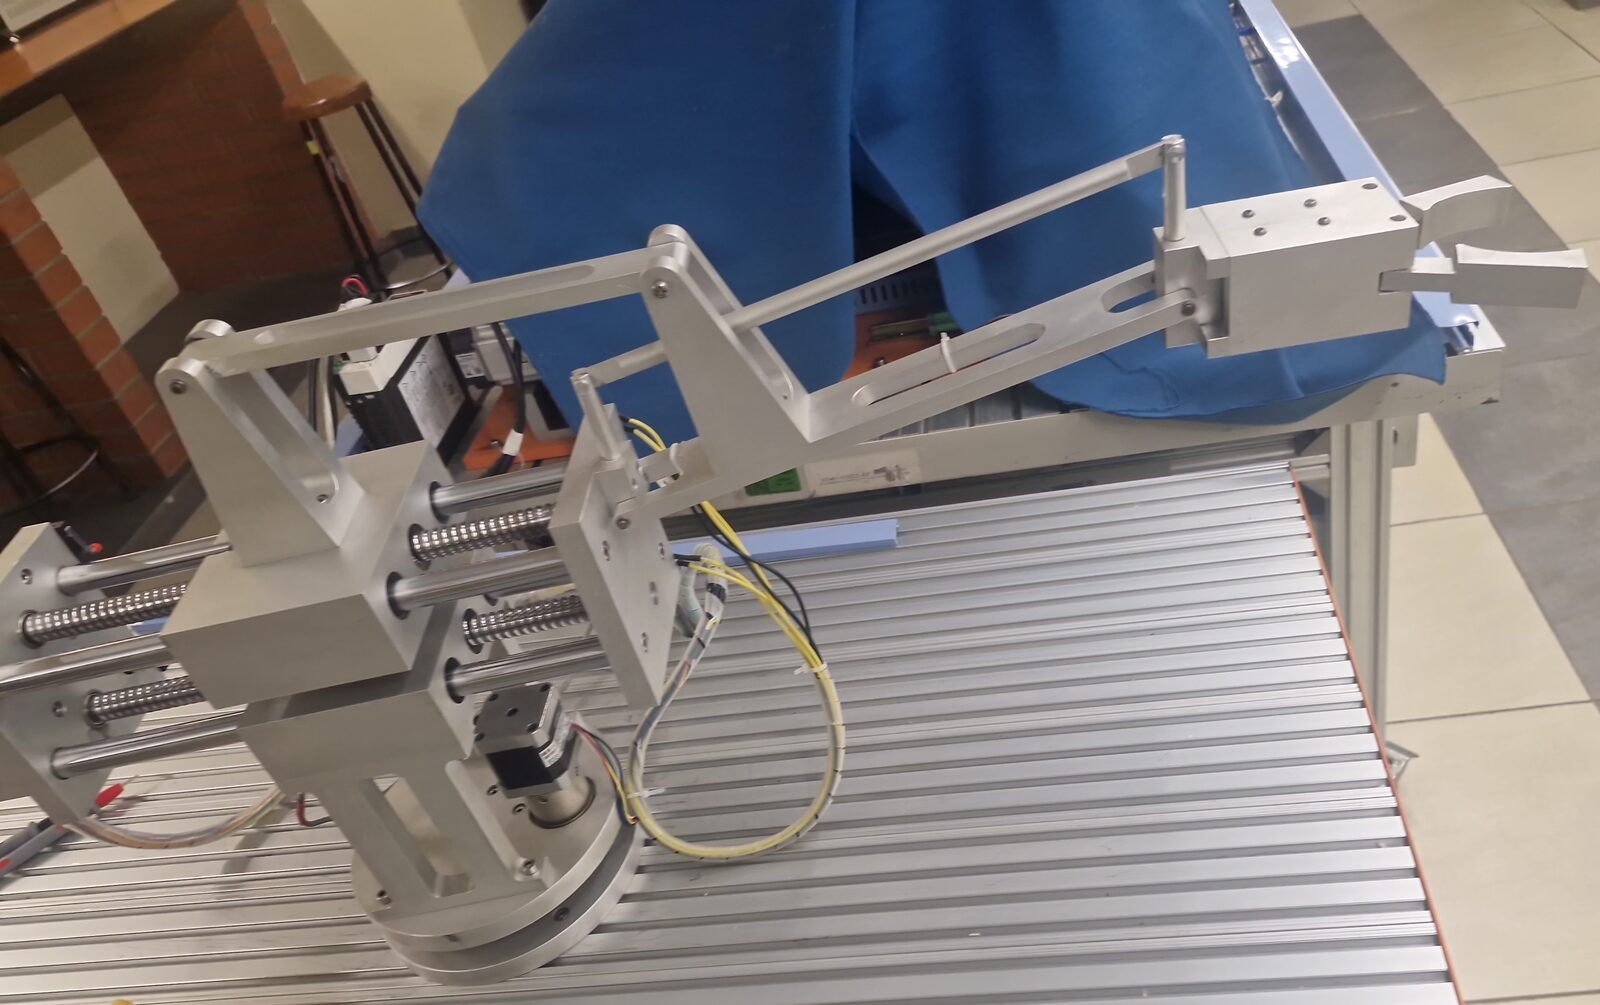
\includegraphics[width=0.78\linewidth]{brazo_vista_general.jpg}\par
\vspace{0.8cm}
{\large Programas ladder · drivers y frecuencias · cinemática y jacobiano · protocolo PPI\\ aplicaciones · base de datos · estructura del proyecto\par}
\vfill
{\large ETN-902 Sistemas de Control II · ETN-1034 Aplicación de Técnicas de Control · ETN-1000 Bases de Datos\par}
\vspace{0.2cm}
{\large Gestión II/2026 · La Paz, 10 de noviembre de 2026\par}
\end{titlepage}

\tableofcontents
\listoffigures
\listoftables

% =====================================================================
\chapter{Objetivos y cómo usar este manual}\label{cap:objetivos}

Este manual reúne, en un solo documento, todo el conocimiento técnico del brazo robótico XK-JS1-1 del laboratorio y del gemelo digital desarrollado sobre él durante la gestión II/2026: el hardware y su cableado, la configuración de los drivers y las frecuencias de trabajo, los dos programas ladder del PLC explicados red por red, el modelo cinemático con su jacobiano, el protocolo de comunicación entre la computadora y el PLC, las aplicaciones de software, la base de datos y la estructura del repositorio.

Está escrito para que un estudiante que llegue al laboratorio sin conocer el brazo pueda entenderlo por completo, reproducir los resultados y continuar el trabajo.

\section{Marco: el laboratorio integrado}
Las guías de laboratorio del semestre (carpeta \codigo{semestres/2026\_II/guias/} del repositorio) organizan el trabajo de tres asignaturas sobre las mismas plantas, siguiendo el Ciclo de Vida del Desarrollo de Sistemas (SDLC) y la mejora continua (Kaizen):

\begin{center}\small
\begin{tabularx}{\linewidth}{>{\raggedright}p{3.1cm} >{\raggedright\arraybackslash}X}
\toprule
\textbf{Asignatura} & \textbf{Responsabilidad sobre el brazo}\\
\midrule
ETN-902 Control II & caracterización, modelado matemático, linealización, identificación de variables y lazos\\
ETN-1034 Aplicación de Técnicas & programación del PLC (PTO), cableado de drivers y sensores, control avanzado, comunicaciones industriales\\
ETN-1000 Bases de Datos & modelo de datos de telemetría, interfaces (HMI y web), conectividad entre la planta y el servidor\\
\bottomrule
\end{tabularx}
\end{center}

\begin{figure}[H]
\centering
\begin{tikzpicture}[node distance=4mm and 4mm, fase/.style={draw, rounded corners=2pt, fill=gris, text width=4.6cm, align=left, font=\scriptsize, inner sep=5pt, minimum height=26mm}]
\node[fase] (f1) {\textbf{Fase 1 · semanas 1--6}\\Ingeniería inversa y auditoría Kaizen\\[2pt] Lab 1: auditoría, variables PV/MV/DV, causalidad\\ Lab 2: planos ISA/IEC, mockups\\ Lab 3: Git/GitHub, modelo E-R en 3FN};
\node[fase, right=of f1] (f2) {\textbf{Fase 2 · semanas 7--13}\\Modelado dinámico y backend\\[2pt] modelado, linealización de los brazos, redes de Petri, scripts SQL, triggers\\ \textbf{Hito}: gemelos digitales validados en simulación};
\node[fase, right=of f2, fill=naranja!12] (f3) {\textbf{Fase 3 · semanas 14--20}\\Implementación y redes\\[2pt] lazos en el hardware real, comunicación PLC--PC, middleware Python, telemetría, dashboard};
\draw[flecha] (f1) -- (f2); \draw[flecha] (f2) -- (f3);
\end{tikzpicture}
\caption{Fases del semestre según la guía 1.}
\end{figure}

\section{Qué objetivo cubre cada capítulo}
\begin{center}\small
\begin{longtable}{>{\raggedright}p{6.6cm} >{\raggedright\arraybackslash}p{8.6cm}}
\toprule
\textbf{Objetivo de las guías} & \textbf{Dónde se cubre}\\
\midrule
\endhead
Identificar y clasificar variables PV, MV, DV; ruptura de causalidad (Lab 1) & Capítulo \ref{cap:planta}: variables, tags ISA, lazo abierto con supervisión discreta\\
Ficha técnica del hardware, ingeniería inversa (Lab 1) & Capítulos \ref{cap:planta} y \ref{cap:drivers}\\
Planos eléctricos, potencia y mando, bornes al PLC (Lab 2) & Capítulo \ref{cap:electrico}\\
Programación del PLC: PTO, temporizadores, secuencias (ETN-1034) & Capítulos \ref{cap:s7200}, \ref{cap:original} y \ref{cap:gemeloplc}\\
Redes de Petri para comportamiento secuencial (Fase 2) & Sección \ref{sec:petri}\\
Modelado y linealización de los brazos (Fase 2) & Capítulo \ref{cap:cinematica}: cinemática, jacobiano, linealización\\
Gemelo digital validado (hito de la Fase 2) & Capítulos \ref{cap:cinematica}, \ref{cap:aplicaciones} y \ref{cap:mediciones}\\
Comunicación PLC--PC, tramas binarias (Fase 3) & Capítulo \ref{cap:ppi}: protocolo PPI byte a byte\\
Middleware en Python, arquitectura de 3 capas (Lab 1, Fase 3) & Capítulo \ref{cap:aplicaciones}\\
Modelo E-R normalizado en 3FN, scripts SQL, triggers (Lab 3, Fase 2) & Capítulo \ref{cap:datos}\\
Control de acceso por roles (Fase 3) & Secciones \ref{sec:acceso} y \ref{sec:tablas}\\
Estructura del repositorio, Git y GitHub (Lab 3) & Capítulo \ref{cap:proyecto}\\
Variables medidas y resultados & Capítulo \ref{cap:mediciones}\\
Balance de cumplimiento & Capítulo \ref{cap:cumplimiento}\\
\bottomrule
\end{longtable}
\end{center}

\section{Convenciones}
\begin{itemize}
\item \textbf{SUPUESTO}: dato que no se midió en la planta y se tomó de una estimación o del fabricante. Debe verificarse.
\item \textbf{Ejes}: la \emph{base} gira un ángulo $\theta$ y su motor se llama \emph{eje Z} (así lo nombran el informe 1 y la app); los \emph{carros X e Y} son lineales. La garra es el cuarto grado de libertad (binario).
\item Direcciones del PLC en notación Siemens: \codigo{I0.5} entrada, \codigo{Q0.1} salida, \codigo{M5.0} marca, \codigo{VB1100} byte de la memoria V, \codigo{VW} palabra (2 bytes), \codigo{VD} doble palabra (4 bytes), \codigo{SM} memoria especial, \codigo{T} temporizador.
\item Los fragmentos de código están copiados de los archivos reales del repositorio; los programas del PLC completos están en los apéndices.
\end{itemize}

\section{Documentos relacionados}
\begin{center}\small
\begin{tabularx}{\linewidth}{>{\raggedright}p{6.2cm} >{\raggedright\arraybackslash}X}
\toprule
\textbf{Documento} & \textbf{Contenido}\\
\midrule
\codigo{manual\_linux.pdf}, \codigo{manual\_windows.pdf} & instalación y uso de la app del gemelo\\
\codigo{arquitectura\_gemelo\_digital.pdf} & por qué se diseñó así: páginas, puertas de acceso\\
\codigo{guia\_completa\_brazo.pdf} & versión resumida de este manual\\
\codigo{informes/informe\_1\_auditoria\_y\_requerimientos.pdf} & auditoría inicial del equipo (Lab 1)\\
\codigo{modelo-3d/informe/informe\_cinematica\_modelo\_3d.pdf} & desarrollo del modelo cinemático y 3D\\
\codigo{global/datasheets/} & hojas de datos de PLC, drivers, sensores y relés\\
\bottomrule
\end{tabularx}
\end{center}

% =====================================================================
\chapter{La planta}\label{cap:planta}

\section{Qué es y qué hace}
El XK-JS1-1 es un brazo didáctico de \textbf{4 grados de libertad} que toma piezas pequeñas y las traslada. Tres movimientos son continuos y accionados por motores paso a paso; el cuarto es la garra, de dos estados.

\begin{figure}[H]
\centering
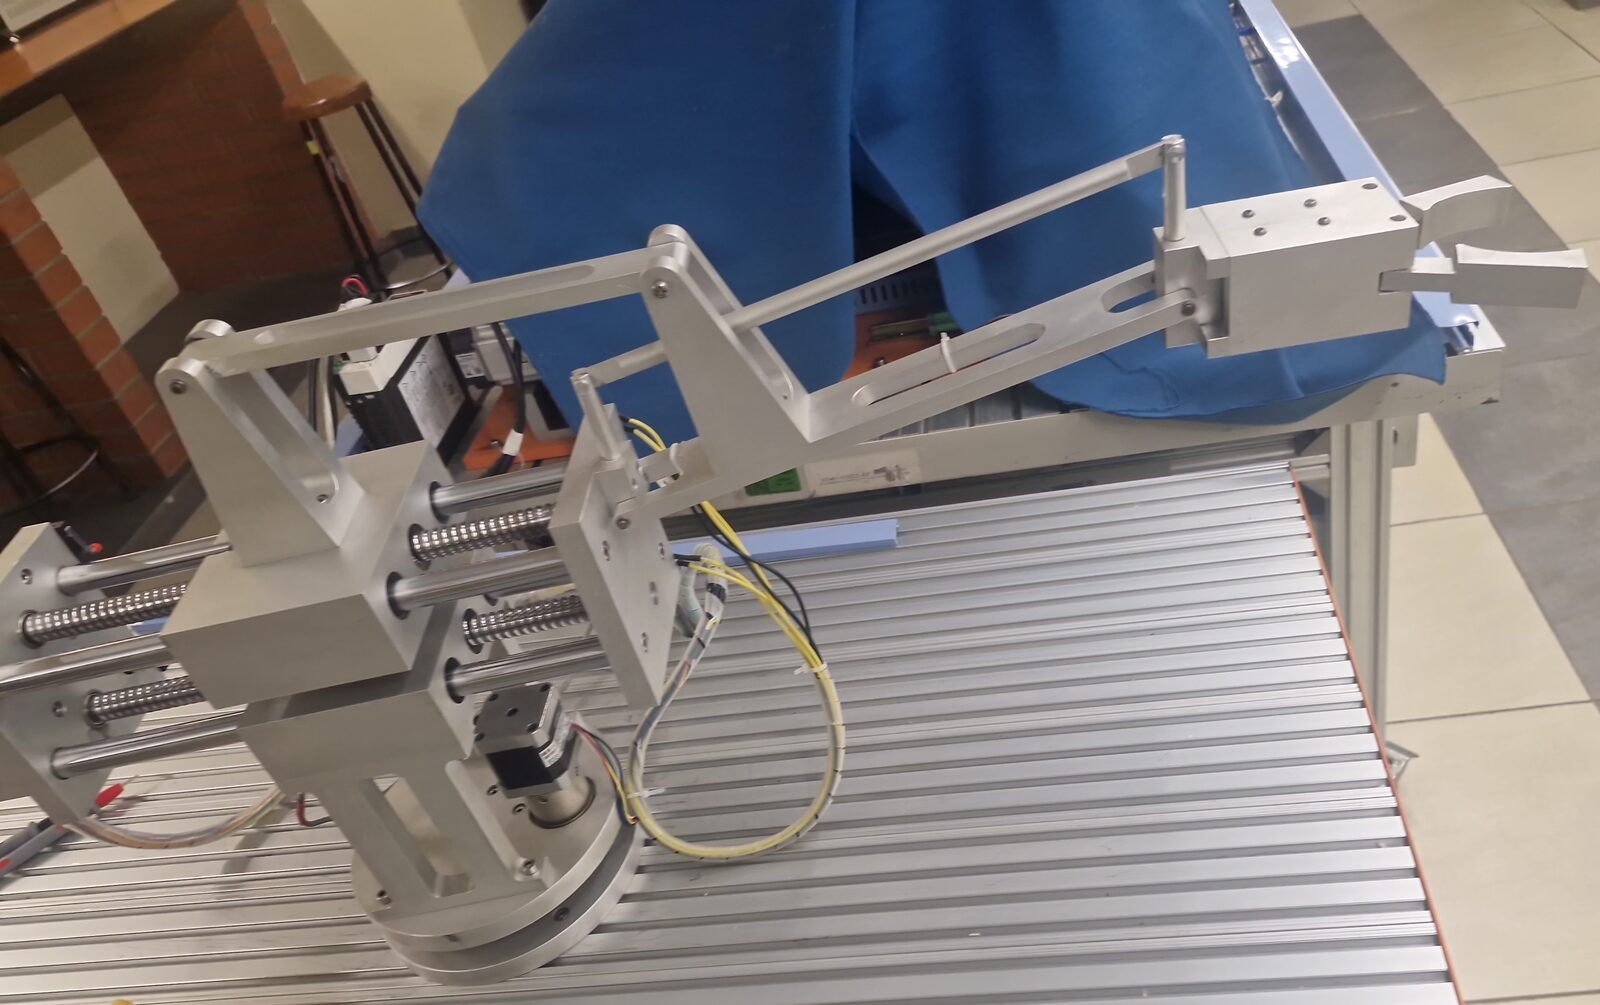
\includegraphics[width=0.62\linewidth]{brazo_vista_general.jpg}
\caption{El brazo XK-JS1-1 en el laboratorio.}
\end{figure}

\begin{center}\small
\begin{tabularx}{\linewidth}{>{\raggedright}p{2.5cm} >{\raggedright}X >{\raggedright\arraybackslash}p{4.8cm}}
\toprule
\textbf{Grado de libertad} & \textbf{Movimiento} & \textbf{Accionamiento}\\
\midrule
Base ($\theta$, motor Z) & giro alrededor del eje vertical & NEMA 17 + driver 2M530 + engranaje\\
Carro X ($s_X$) & desplaza todo el brazo: cambia el alcance & NEMA 23 + driver 2M542 + husillo inferior\\
Carro Y ($s_Y$) & mueve un bloque que, por una biela, levanta el brazo: cambia la altura & NEMA 23 + driver 2M542 + husillo superior\\
Garra & abre o cierra las mordazas & solenoide de 24~V por el relé K3 (salida Q0.7)\\
\bottomrule
\end{tabularx}
\end{center}

\section{Ficha técnica del hardware}
Datos de la auditoría del informe 1, de las hojas de datos de \codigo{global/datasheets/} y de las verificaciones hechas en la planta en octubre de 2026.

\begin{center}\small
\begin{longtable}{>{\raggedright}p{3.2cm} >{\raggedright}p{4cm} >{\raggedright\arraybackslash}p{7.8cm}}
\toprule
\textbf{Componente} & \textbf{Modelo} & \textbf{Datos clave}\\
\midrule
\endhead
PLC & Siemens S7-200 CPU 224 CN (6ES7 214-1AD23) & 14 entradas y 10 salidas digitales de 24~V DC (transistor); 2 salidas de pulsos rápidas (Q0.0, Q0.1) hasta 20~kHz; un puerto RS-485 (puerto 0) con protocolo PPI\\
Drivers X e Y & JMC 2M542-N (compatible DM542) & 20--50~V DC, 1,0--4,2~A pico; entradas PUL, DIR y ENA optoacopladas; micropasos por interruptores DIP\\
Driver base & JMC 2M530 & 18--50~V DC, 0,5--3,0~A (informe 1); tabla DIP por confirmar en su placa\\
Motores X e Y & NEMA 23, 57J1854-828 & 1,8° por paso (200 pasos/vuelta), 2,8~A por fase\\
Motor base & NEMA 17, 42J1848-604 & 1,8° por paso, 1,2~A por fase\\
Husillos X e Y & de bolas, tipo SFU1605 (SUPUESTO) & paso 5~mm/vuelta (SUPUESTO)\\
Relés K1, K2, K3 & Omron MY2N-J (24~V DC) & 2 contactos conmutados (DPDT), 5~A; K1 y K2 reparten el tren de pulsos, K3 acciona el solenoide\\
Finales de carrera X e Y & microinterruptores (informe 1: M102-011; hoja de datos: V-156-1C25) & 4 unidades, contacto NA/NC\\
Sensor de la base & LJ12A3-4-Z/BX & inductivo NPN normalmente abierto, 6--36~V DC, alcance 4~mm, 100~Hz\\
Garra & solenoide de 24~V DC & todo o nada; Q0.7 = 1 cerrada\\
Fuente & conmutada 24~V / 5~V DC & alimenta PLC, sensores y la lógica de los drivers\\
Protección & disyuntor diferencial DZ47LE-63 & 16~A, 30~mA, curva C\\
Panel & botonera & pulsadores Start, Stop, Reset, S1--S7 y selector Manual/Automático\\
\bottomrule
\end{longtable}
\end{center}

\begin{figure}[H]
\centering
\begin{minipage}[t]{0.32\linewidth}\centering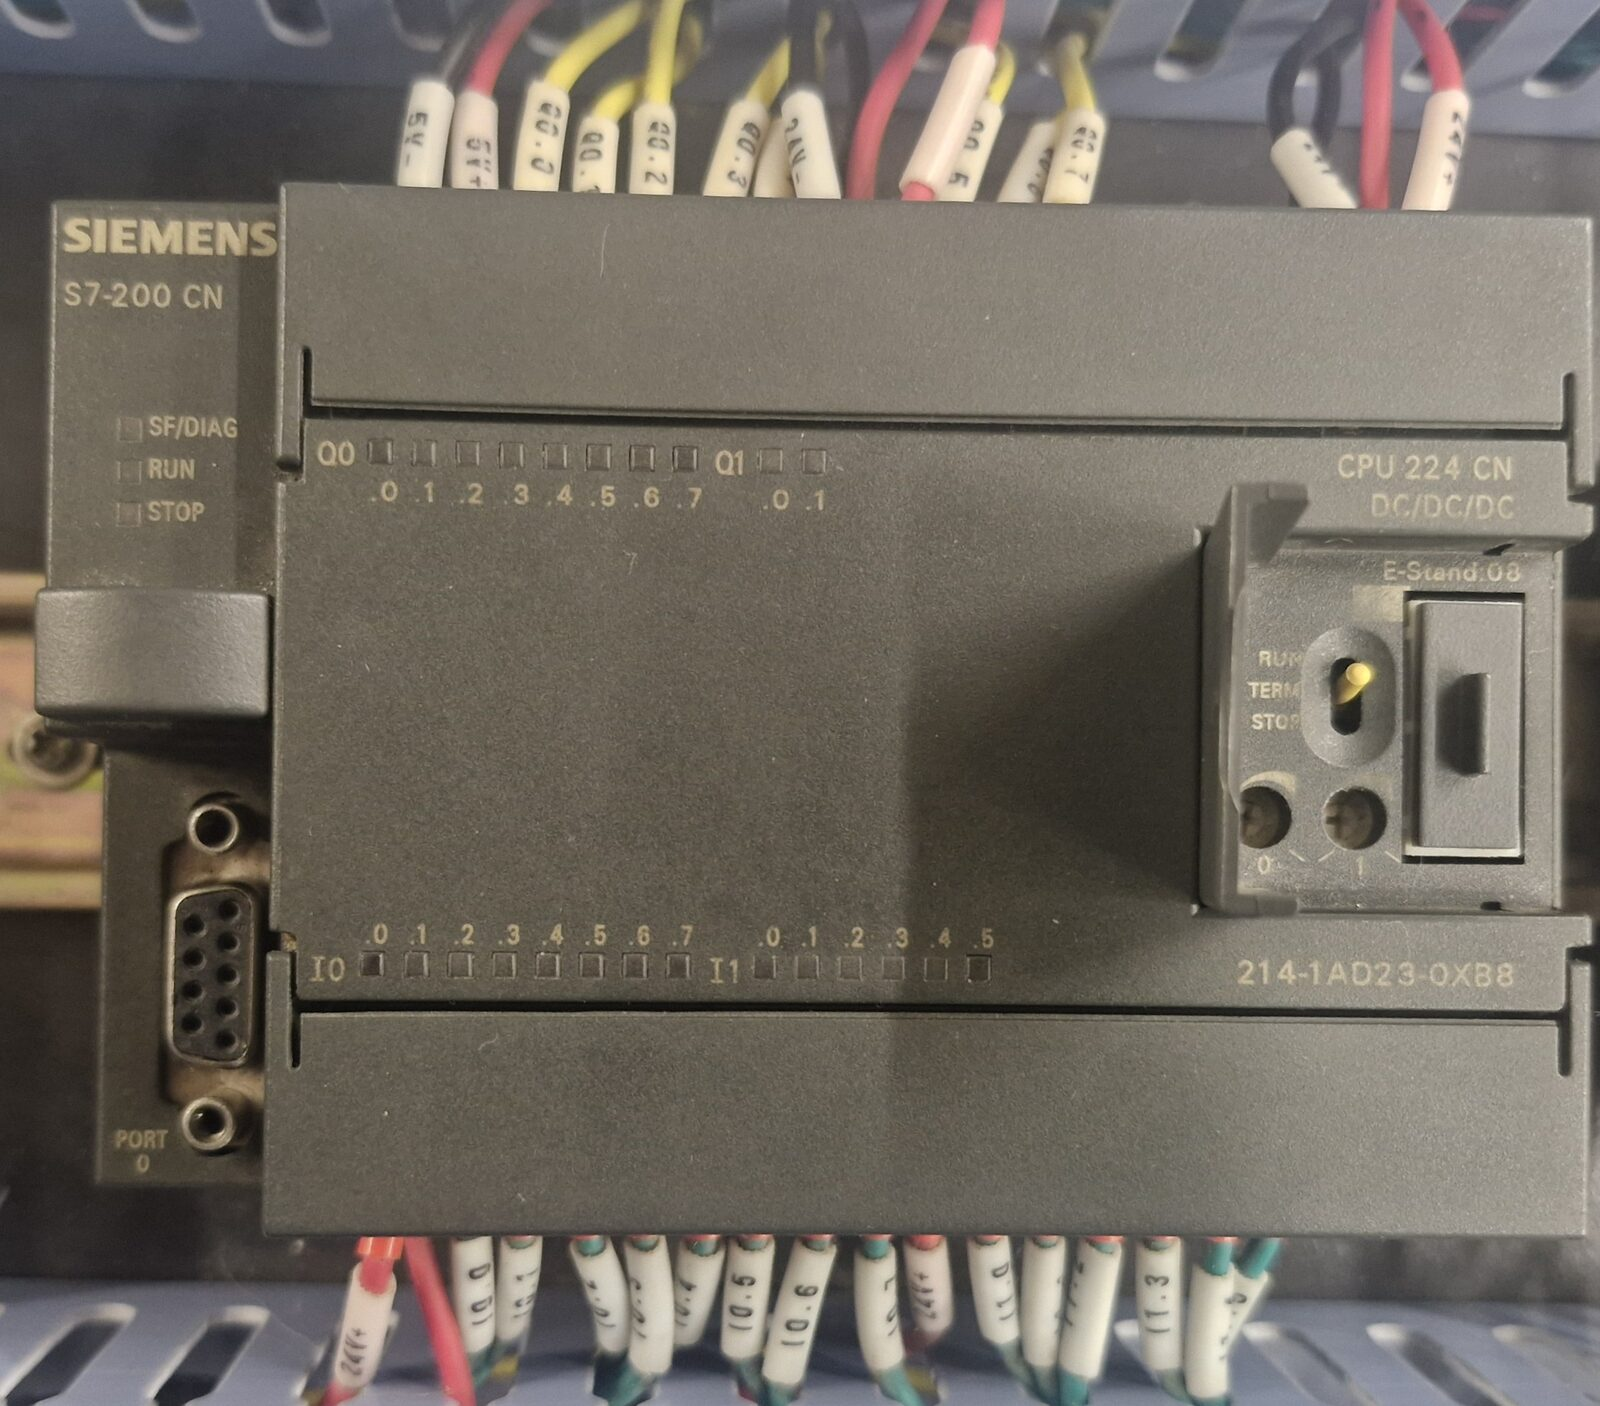
\includegraphics[width=\linewidth, height=3.6cm, keepaspectratio]{plc_s7-200_cpu224.jpg}\\{\small (a) PLC S7-200 CPU 224}\end{minipage}\hfill
\begin{minipage}[t]{0.32\linewidth}\centering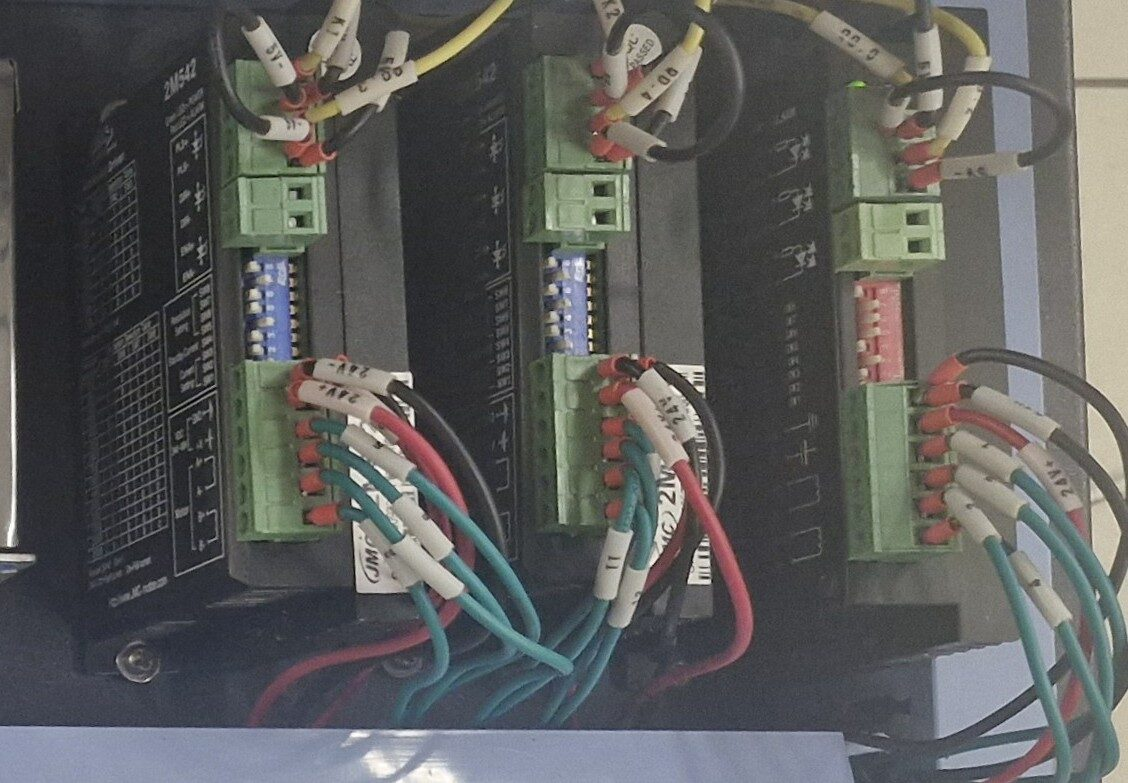
\includegraphics[width=\linewidth, height=3.6cm, keepaspectratio]{drivers_2m542_2m530.jpg}\\{\small (b) drivers 2M542 y 2M530}\end{minipage}\hfill
\begin{minipage}[t]{0.32\linewidth}\centering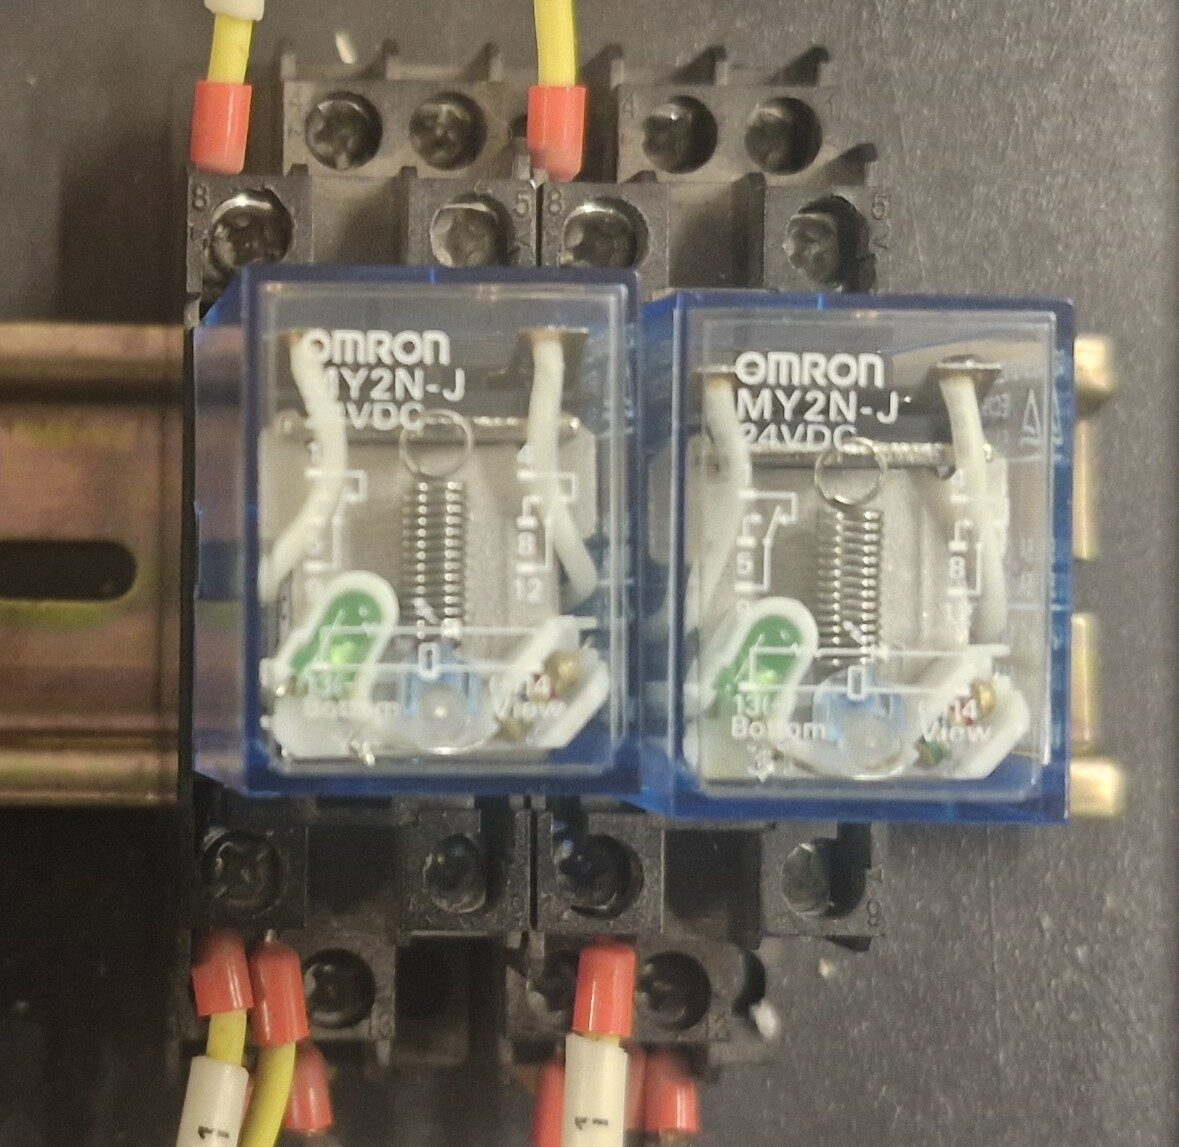
\includegraphics[width=\linewidth, height=3.6cm, keepaspectratio]{reles_omron_my2nj.jpg}\\{\small (c) relés Omron MY2N-J}\end{minipage}\\[6pt]
\begin{minipage}[t]{0.32\linewidth}\centering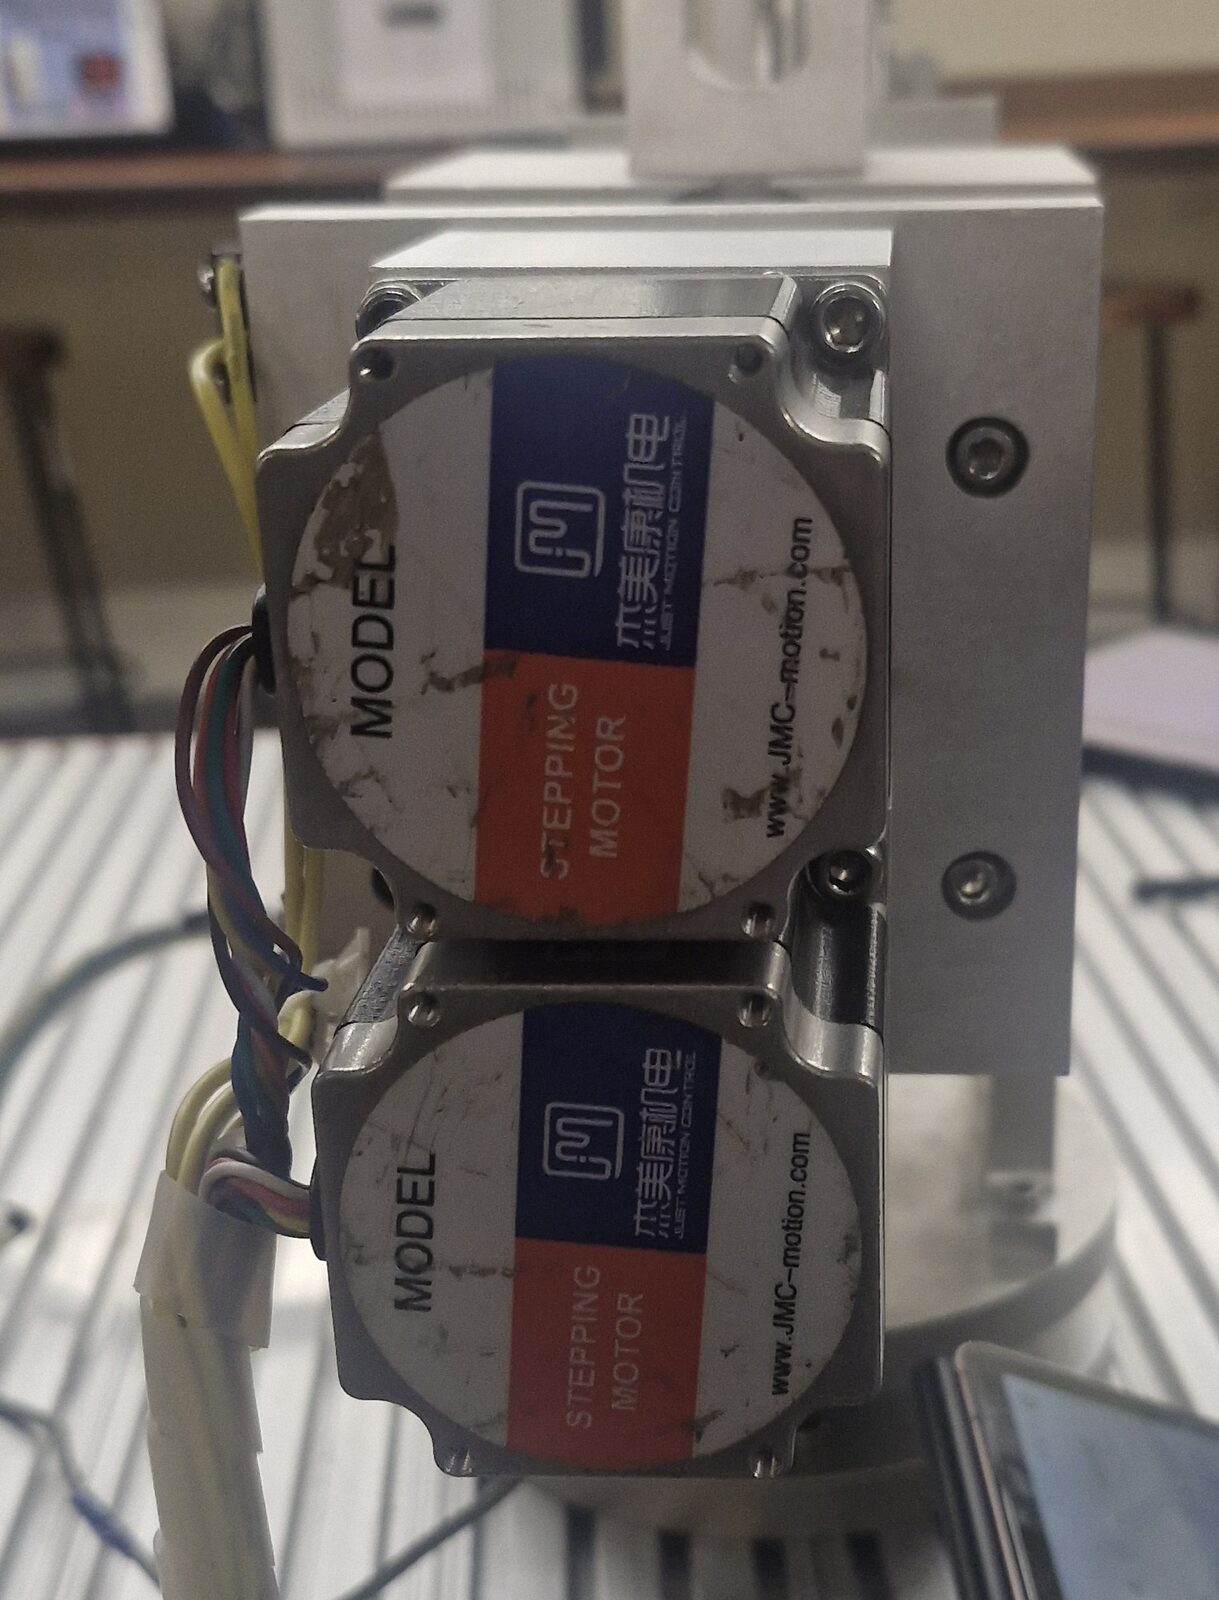
\includegraphics[width=\linewidth, height=3.6cm, keepaspectratio]{motores_nema23_ejes_xy.jpg}\\{\small (d) motores NEMA 23 (X, Y)}\end{minipage}\hfill
\begin{minipage}[t]{0.32\linewidth}\centering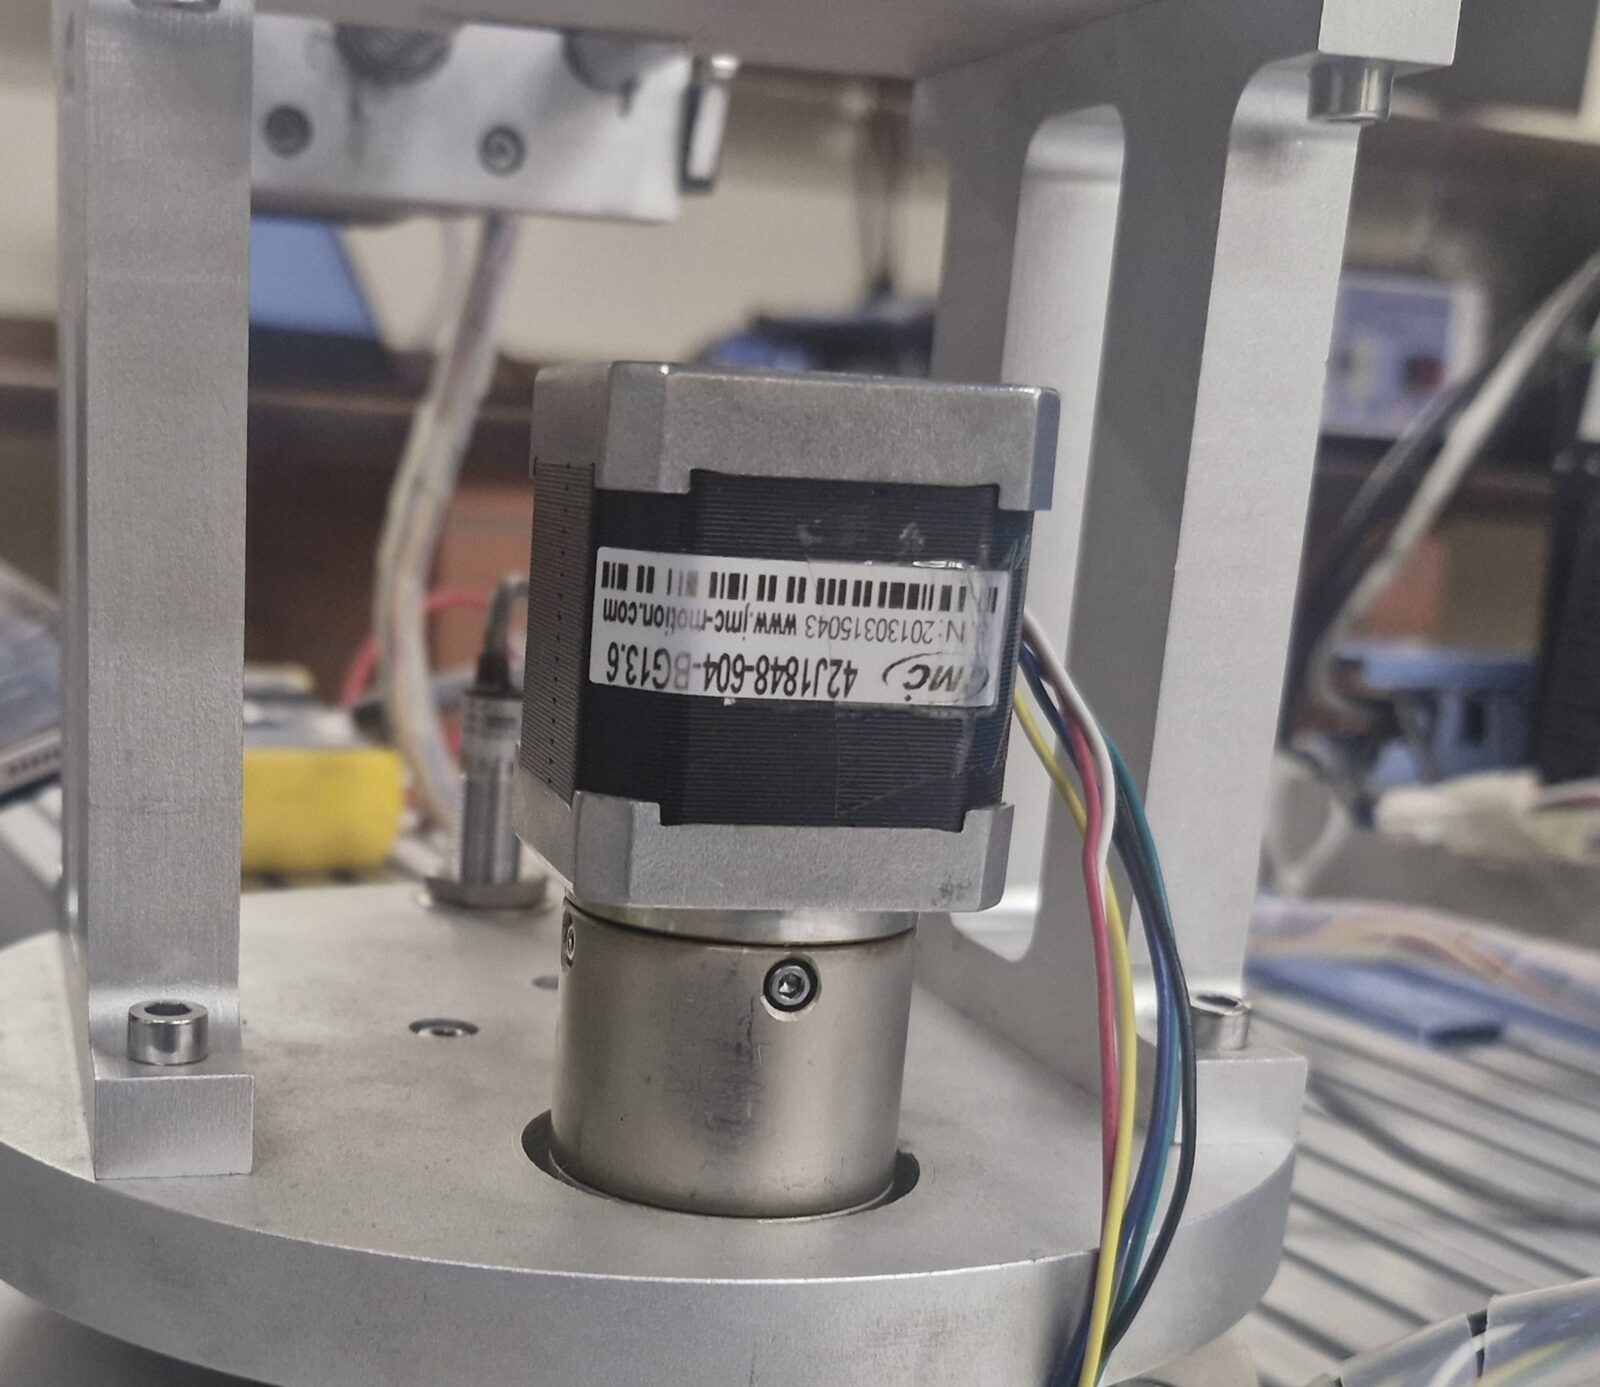
\includegraphics[width=\linewidth, height=3.6cm, keepaspectratio]{motor_nema17_eje_z.jpg}\\{\small (e) motor NEMA 17 (base)}\end{minipage}\hfill
\begin{minipage}[t]{0.32\linewidth}\centering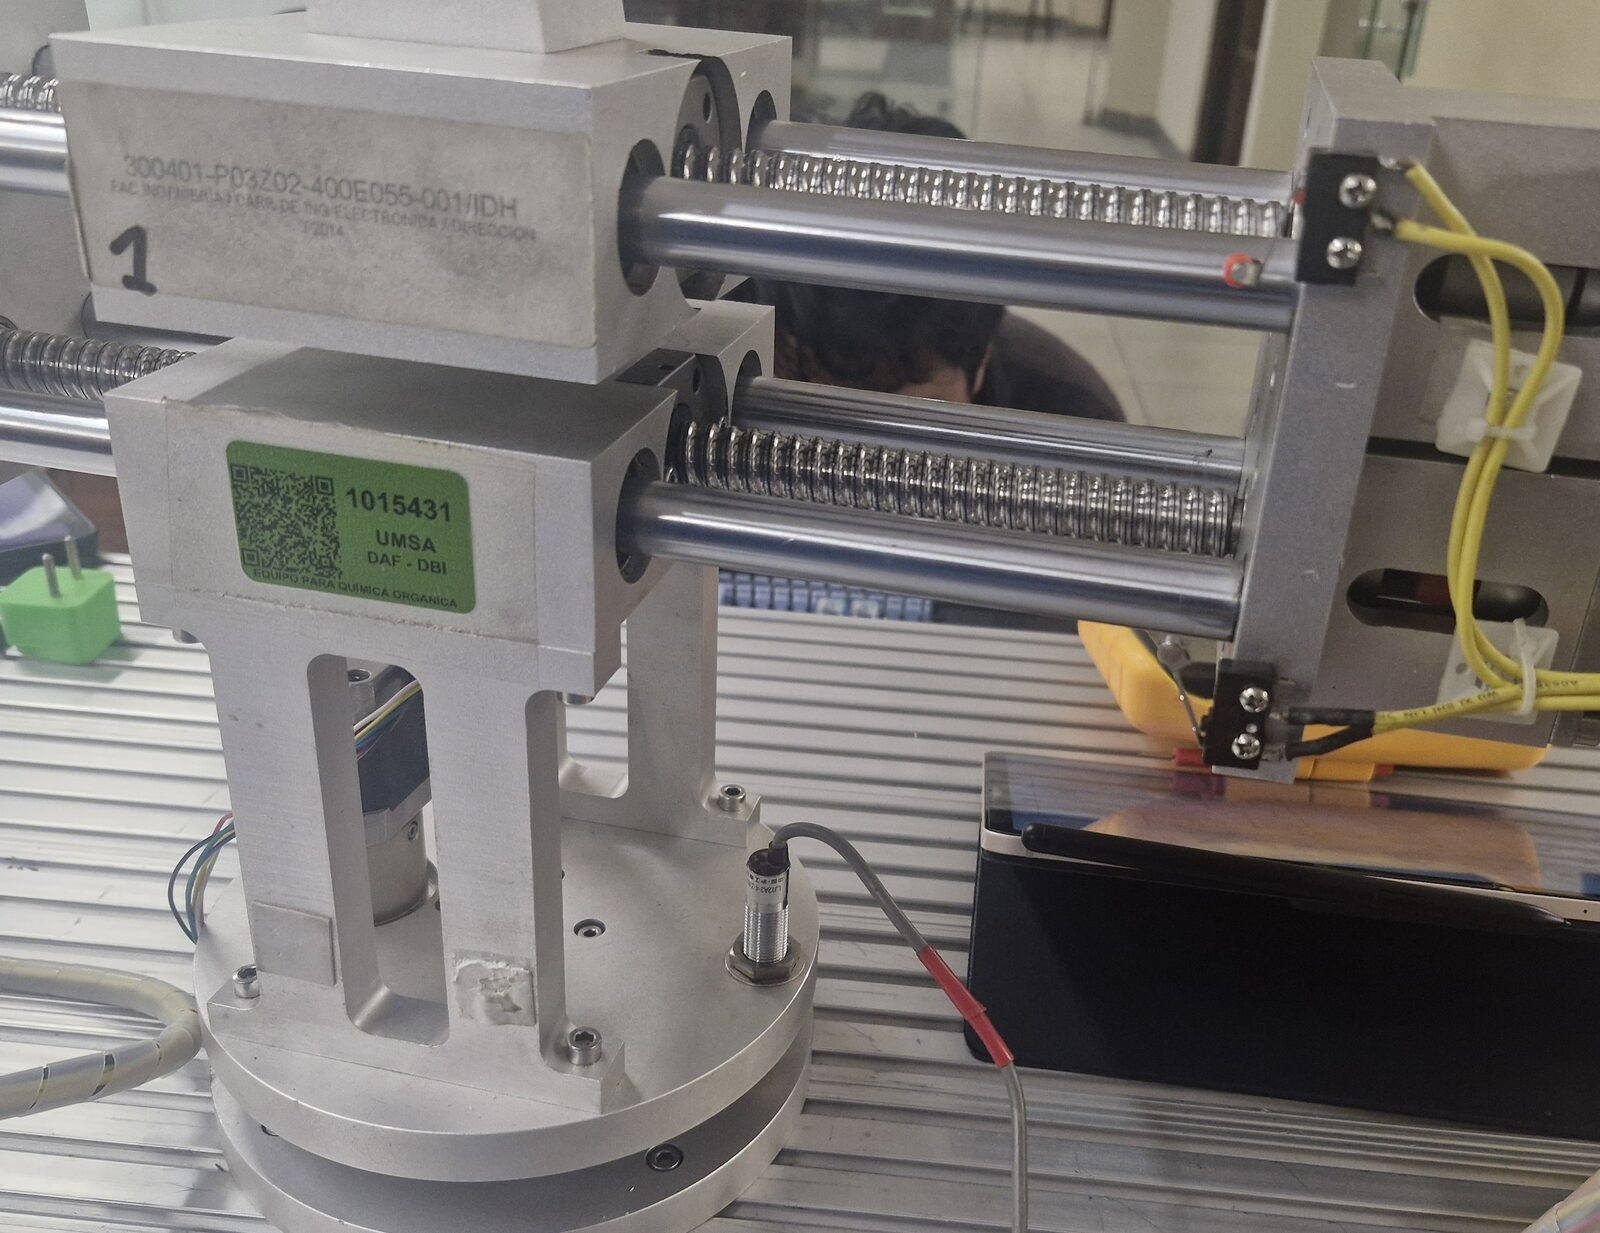
\includegraphics[width=\linewidth, height=3.6cm, keepaspectratio]{eje_z_sensor_inductivo.jpg}\\{\small (f) sensor inductivo de la base}\end{minipage}\\[6pt]
\begin{minipage}[t]{0.32\linewidth}\centering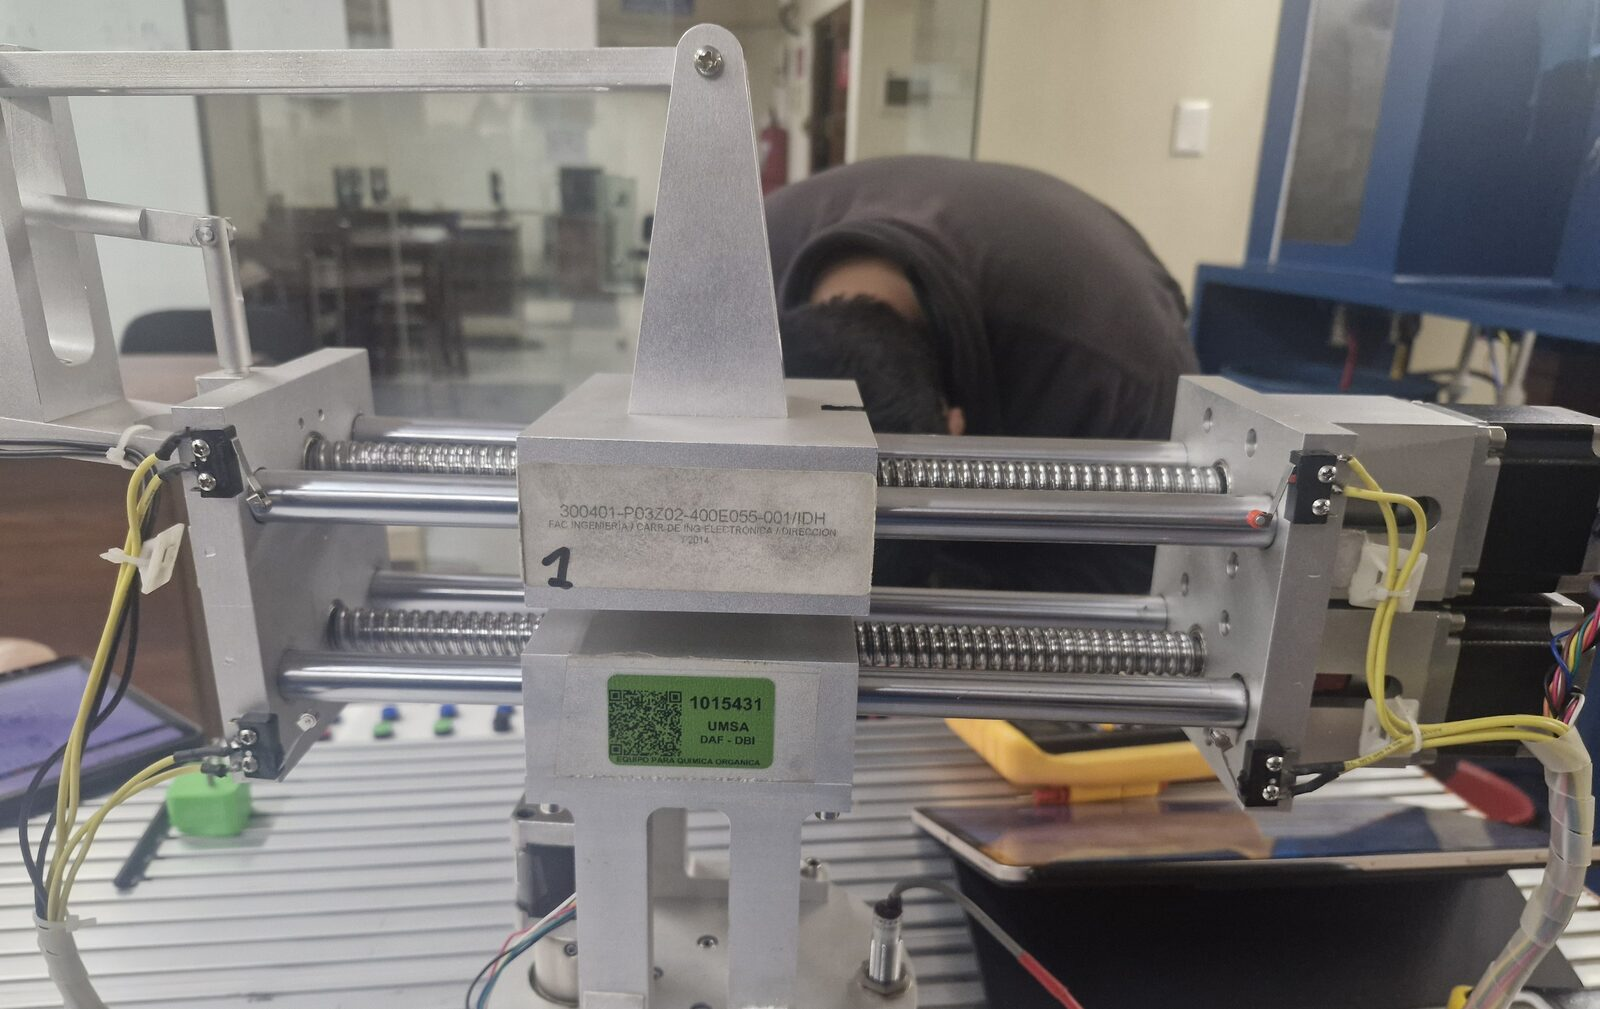
\includegraphics[width=\linewidth, height=3.6cm, keepaspectratio]{final_de_carrera_rieles_xy.jpg}\\{\small (g) finales de carrera X e Y}\end{minipage}\hfill
\begin{minipage}[t]{0.32\linewidth}\centering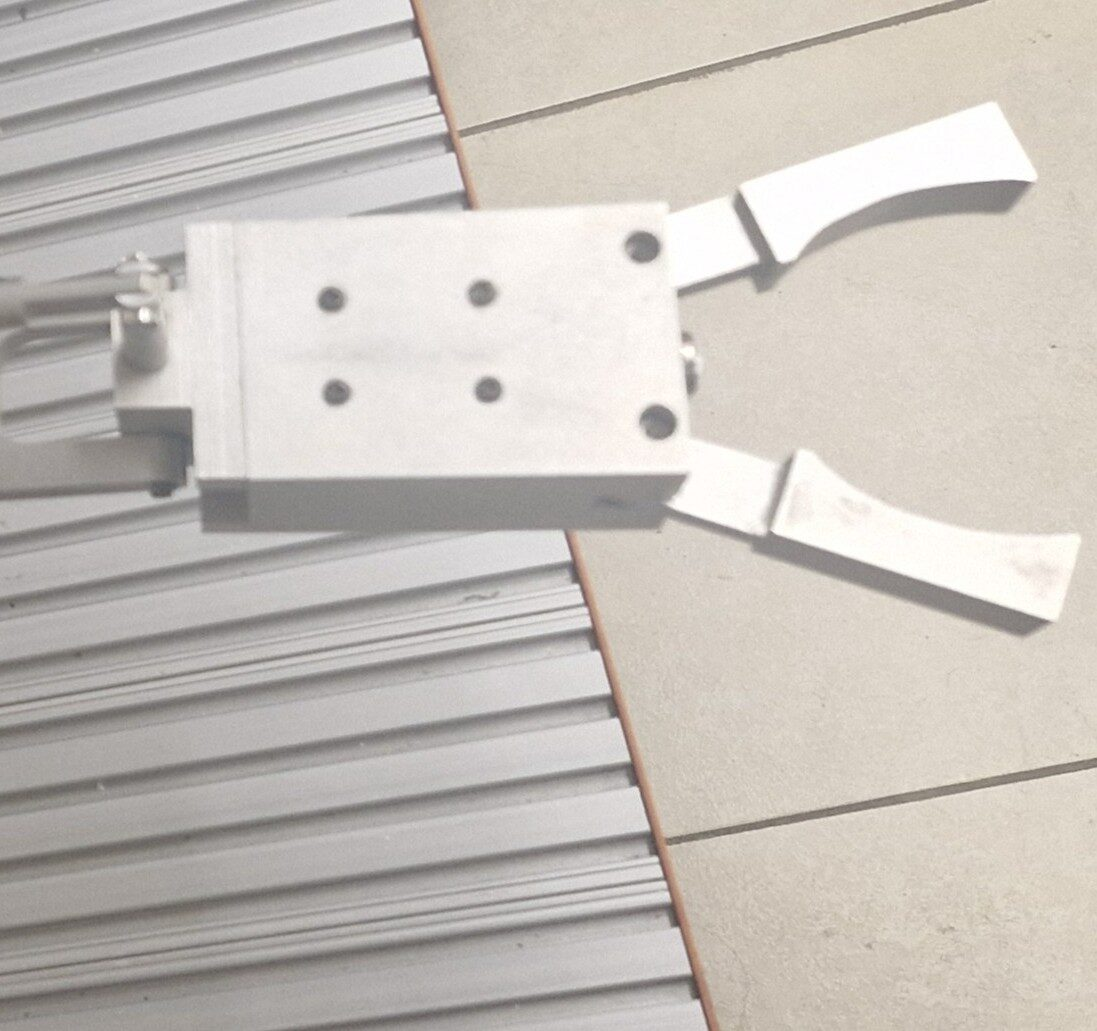
\includegraphics[width=\linewidth, height=3.6cm, keepaspectratio]{garra_solenoide.jpg}\\{\small (h) garra}\end{minipage}\hfill
\begin{minipage}[t]{0.32\linewidth}\centering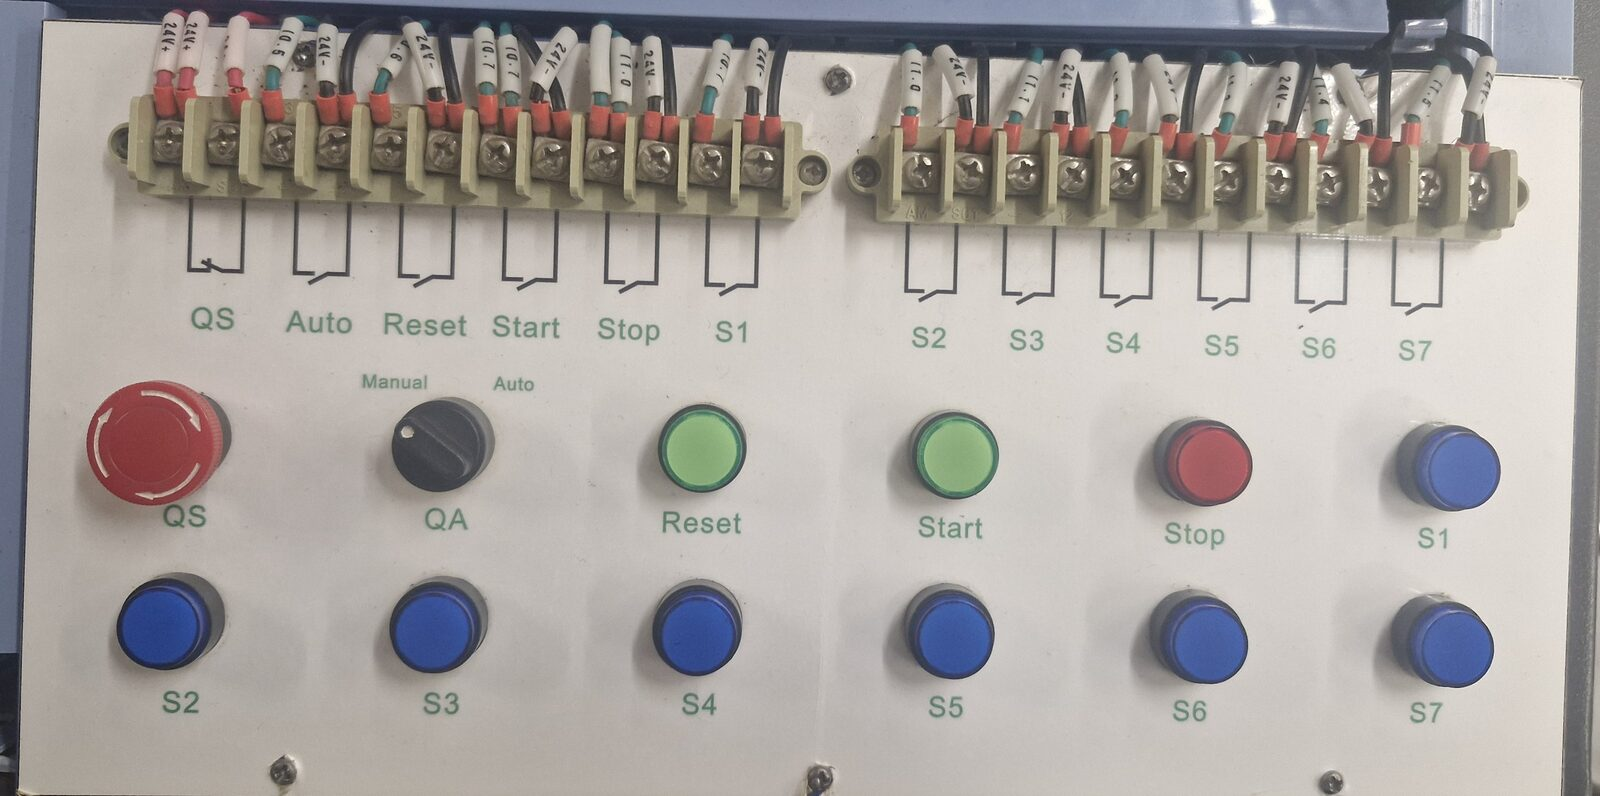
\includegraphics[width=\linewidth, height=3.6cm, keepaspectratio]{botonera.jpg}\\{\small (i) botonera}\end{minipage}
\caption{Componentes de la planta (fotos de \texttt{global/fotos-planta/}).}
\end{figure}

\section{Diagrama de bloques}
\begin{figure}[H]
\centering
\begin{tikzpicture}[node distance=7mm and 10mm]
\node[cajan, text width=3.1cm, minimum height=26mm] (plc) {\textbf{PLC S7-200}\\CPU 224 CN\\14 entradas\\10 salidas\\2 salidas de pulsos};
\node[caja, text width=2.6cm, above left=4mm and 14mm of plc] (panel) {panel:\\selector, paro,\\garra/inicio,\\6 pulsadores};
\node[caja, text width=2.6cm, below left=4mm and 14mm of plc] (sens) {finales de carrera X e Y\\sensor inductivo\\de la base};
\node[caja, text width=2.4cm, right=16mm of plc, yshift=16mm] (dz) {driver base\\2M530};
\node[caja, text width=2.4cm, right=16mm of plc, yshift=-4mm] (k) {relés K1 / K2\\reparten Q0.1};
\node[caja, text width=2.4cm, right=10mm of k, yshift=6mm] (dx) {driver X\\2M542};
\node[caja, text width=2.4cm, right=10mm of k, yshift=-8mm] (dy) {driver Y\\2M542};
\node[caja, text width=2.4cm, below=10mm of k] (garra) {relé K3 + solenoide\\de la garra};
\node[cajab, text width=1.6cm, right=6mm of dz] (mz) {NEMA 17\\base};
\node[cajab, text width=1.6cm, right=6mm of dx] (mx) {NEMA 23\\X};
\node[cajab, text width=1.6cm, right=6mm of dy] (my) {NEMA 23\\Y};
\node[cajab, text width=2.4cm, below=10mm of plc] (pc) {PC\\(USB-PPI, puerto 0)};
\draw[flecha] (panel) -- node[above, etiq, sloped]{I0.5--I1.5} (plc);
\draw[flecha] (sens) -- node[below, etiq, sloped]{I0.0--I0.4} (plc);
\draw[flecha] (plc.east) ++(0,0.6) -- node[above, etiq]{Q0.0, Q0.2} (dz.west);
\draw[flecha] (plc.east) ++(0,-0.4) -- node[above, etiq]{Q0.1} (k.west);
\draw[flecha] (k) -- node[above, etiq]{K1} (dx.west);
\draw[flecha] (k) -- node[below, etiq]{K2} (dy.west);
\draw[flecha] (plc.south east) -- node[above, etiq, sloped]{Q0.7} (garra.west);
\draw[flecha] (dz) -- (mz); \draw[flecha] (dx) -- (mx); \draw[flecha] (dy) -- (my);
\draw[dflecha] (plc) -- node[left, etiq]{PPI} (pc);
\node[etiq, above=1mm of dx] {DIR Q0.3};
\node[etiq, below=1mm of dy] {DIR Q0.4};
\end{tikzpicture}
\caption{Diagrama de bloques de la planta.}
\end{figure}

\section{Mapa de entradas y salidas verificado}
Cada sensor se accionó a mano mientras un monitor por PPI registraba los cambios (26/10/2026). Esto corrigió el mapa del informe 1 (sección \ref{sec:kaizen}).

\begin{center}\small
\begin{tabularx}{\linewidth}{>{\ttfamily}p{1.1cm} >{\raggedright}X >{\ttfamily}p{1.1cm} >{\raggedright\arraybackslash}X}
\toprule
\textbf{\rmfamily Entrada} & \textbf{Función} & \textbf{\rmfamily Salida} & \textbf{Función}\\
\midrule
I0.0 & sensor inductivo de la base ($\theta = 0$) & Q0.0 & pulsos de la base (PTO0)\\
I0.1 & final X atrás (origen) & Q0.1 & pulsos de X e Y (PTO1), compartidos\\
I0.2 & final X adelante & Q0.2 & DIR base (1 = hacia el inductivo)\\
I0.3 & final Y abajo (origen) & Q0.3 & DIR X (0 = adelante)\\
I0.4 & final Y arriba & Q0.4 & DIR Y (0 = arriba)\\
I0.5 & selector: 0 manual, 1 automático/remoto & Q0.5 & relé K1: Q0.1 al driver X\\
I0.6 & paro & Q0.6 & relé K2: Q0.1 al driver Y\\
I0.7 & garra / inicio & Q0.7 & relé K3: solenoide (1 = cerrada)\\
I1.0 / I1.1 & jog base + / $-$ & & \\
I1.2 / I1.3 & jog X adelante / atrás & & \\
I1.4 / I1.5 & jog Y arriba / abajo & & \\
\bottomrule
\end{tabularx}
\end{center}
La correspondencia entre los rótulos de la botonera (S1--S7, Start, Stop) y las entradas I0.6--I1.5 no se registró pulsador por pulsador (SUPUESTO: Stop = I0.6, Start = I0.7).

\section{Variables del proceso (PV, MV, DV)}
El brazo no tiene sensores de posición continua (encoders): la posición de cada eje se \emph{infiere} contando pulsos. Clasificación corregida respecto del informe 1:

\begin{center}\small
\begin{longtable}{>{\raggedright}p{1.3cm} >{\raggedright}p{4.2cm} >{\raggedright\arraybackslash}p{9.4cm}}
\toprule
\textbf{Tipo} & \textbf{Variable} & \textbf{Señal física y rango}\\
\midrule
\endhead
MV & tren de pulsos de la base ($N_\theta$, $f_\theta$) & Q0.0 (PTO0), 0--20~kHz; se usa 2,5--4~kHz\\
MV & tren de pulsos de X e Y ($N_{XY}$, $f_{XY}$) & Q0.1 (PTO1), uno solo para los dos carros\\
MV & selección de carro & Q0.5 (K1, carro X), Q0.6 (K2, carro Y)\\
MV & dirección de cada eje & Q0.2 (base), Q0.3 (X), Q0.4 (Y)\\
MV & garra & Q0.7, 24~V al relé K3\\
PV & posición de la base $\theta$ & sin sensor continuo; $\theta = n_\theta / 190{,}3$ [°]\\
PV & posición de los carros $s_X$, $s_Y$ & sin sensor continuo; $s = n / 200$ [mm], 0--170~mm\\
PV & posición de la garra $(X, Y, Z)$ & calculada con la cinemática directa (capítulo \ref{cap:cinematica})\\
PV discreta & referencias de posición & I0.0 (inductivo), I0.1--I0.4 (finales): solo dicen si se alcanzó un punto\\
DV & fricción en guías y husillos & no medible eléctricamente\\
DV & carga en la garra & peso de la pieza: cambia el par que necesita el carro Y\\
DV & pérdida de pasos & arranques sin rampa o sobrecarga: la posición contada deja de ser la real\\
DV & holguras y deformaciones & error de posición de la garra no detectable\\
\bottomrule
\end{longtable}
\end{center}

\section{Lazo abierto con supervisión discreta}
\begin{figure}[H]
\centering
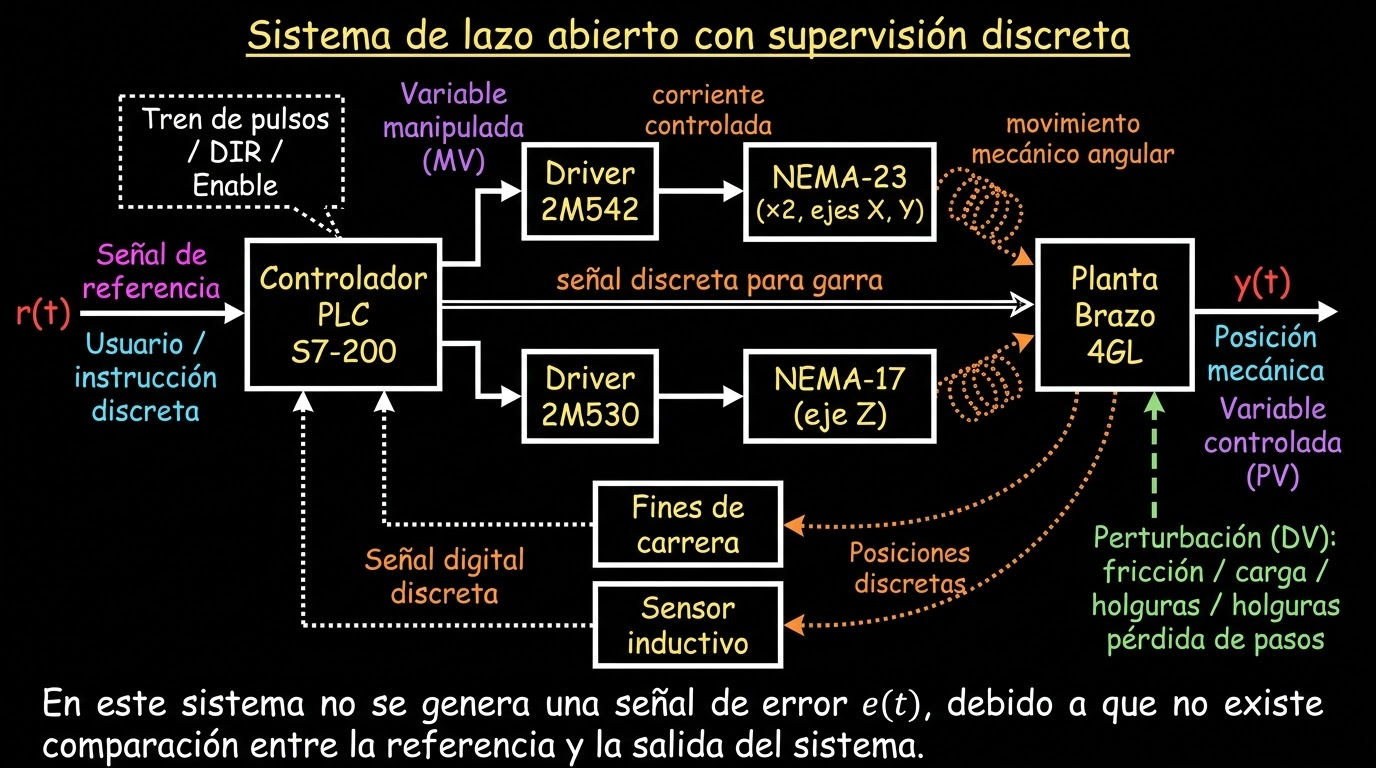
\includegraphics[width=0.8\linewidth]{diagrama_bloques_fenomenologico.png}
\caption{Diagrama de bloques fenomenológico del equipo (\texttt{diagramas/}): no hay realimentación continua de posición.}
\end{figure}
El PLC estima la posición como
\[
q_{est} = q_0 + N_p\,\Delta q ,
\]
donde $q_0$ es la posición de referencia (fijada por el homing), $N_p$ los pulsos enviados y $\Delta q$ el avance por pulso (0,005~mm en los carros). Si el motor pierde pasos, $q_{real} \neq q_{est}$ y el PLC no lo sabe: la acción de control actúa sobre la planta ($u \to y$) pero la salida no vuelve al controlador ($y \not\to u$). Es la \emph{ruptura de causalidad} del informe 1. Los finales de carrera solo corrigen la estimación en puntos aislados. El programa del gemelo aprovecha esto: cada vez que se pisa un final, fija la posición exacta (capítulo \ref{cap:gemeloplc}).

\section{Tags ISA-5.1 propuestos}
Para que los planos, el programa y la base de datos usen los mismos nombres (pedido de las guías 2 y 3), se propone esta identificación. La letra Z de ISA-5.1 designa \emph{posición}; S = interruptor; L/H = bajo/alto; Y = función de cálculo o relé; H = manual; I = indicación; X = sin clasificar.

\begin{center}\small
\begin{longtable}{>{\ttfamily}p{1.9cm} >{\ttfamily}p{1.2cm} >{\raggedright\arraybackslash}p{11cm}}
\toprule
\textbf{\rmfamily Tag} & \textbf{\rmfamily Señal} & \textbf{Descripción}\\
\midrule
\endhead
\multicolumn{3}{@{}l}{\textbf{Lazo 100: general}}\\
HS-100 & I0.5 & selector manual / automático\\
HS-100P & I0.6 & pulsador de paro\\
ZY-100 & Q0.1 & tren de pulsos compartido X/Y (PTO1)\\
\multicolumn{3}{@{}l}{\textbf{Lazo 101: base ($\theta$)}}\\
ZS-101 & I0.0 & interruptor de posición inductivo ($\theta = 0$)\\
HS-101A / B & I1.0 / I1.1 & jog base + / $-$\\
ZY-101 & Q0.0 & tren de pulsos de la base (PTO0)\\
ZY-101D & Q0.2 & dirección de la base\\
ZI-101 & VD1124 & posición de la base (pulsos contados)\\
\multicolumn{3}{@{}l}{\textbf{Lazo 102: carro X}}\\
ZSL-102 / ZSH-102 & I0.1 / I0.2 & final de carrera bajo (atrás) / alto (adelante)\\
HS-102A / B & I1.2 / I1.3 & jog X adelante / atrás\\
ZY-102D & Q0.3 & dirección X\\
ZY-102K & Q0.5 & relé K1\\
ZI-102 & VD1128 & posición X\\
\multicolumn{3}{@{}l}{\textbf{Lazo 103: carro Y}}\\
ZSL-103 / ZSH-103 & I0.3 / I0.4 & final de carrera bajo (abajo) / alto (arriba)\\
HS-103A / B & I1.4 / I1.5 & jog Y arriba / abajo\\
ZY-103D & Q0.4 & dirección Y\\
ZY-103K & Q0.6 & relé K2\\
ZI-103 & VD1132 & posición Y\\
\multicolumn{3}{@{}l}{\textbf{Lazo 104: garra}}\\
HS-104 & I0.7 & garra / inicio\\
XY-104 & Q0.7 & relé K3 del solenoide\\
\bottomrule
\end{longtable}
\end{center}
Los mismos tags están en la base de datos (tablas \codigo{punto\_io} y \codigo{variable}, capítulo \ref{cap:datos}).

\section{Discrepancias Kaizen: versión 2.0}\label{sec:kaizen}
El informe 1 registró discrepancias entre el plano histórico y la planta. La puesta en marcha del gemelo permitió verificarlas con el PLC en marcha y agregar otras:

\begin{center}\small
\begin{longtable}{>{\raggedright}p{0.4cm} >{\raggedright}p{4.4cm} >{\raggedright}p{4.6cm} >{\raggedright\arraybackslash}p{5.6cm}}
\toprule
\textbf{N°} & \textbf{Elemento} & \textbf{Antes} & \textbf{Verificado (oct. 2026)}\\
\midrule
\endhead
1 & finales de carrera & I0.0--I0.3 (informe 1, con desfase de 1 bit) & \textbf{I0.1--I0.4}; I0.0 es el inductivo de la base\\
2 & tren de pulsos de X e Y & Q0.5 (X) y Q0.6 (Y) & \textbf{Q0.1 compartido}; Q0.5 y Q0.6 son los relés K1 y K2 que lo reparten\\
3 & final de homing del carro Y & I0.4 (tabla anterior del proyecto) & \textbf{I0.3} (Y abajo)\\
4 & sentido de X & no documentado & Q0.3 = 0 adelante (se separa de I0.1)\\
5 & dirección PPI del PLC & 7 (proyecto de Miguel) & \textbf{6} a 19,2~kbit/s con el programa original; \textbf{2} a 9,6~kbit/s tras cargar \codigo{brazo\_gemelo} con su bloque de sistema\\
6 & reducción de la base & 5:1 (SUPUESTO del modelo) & \textbf{190,3 pulsos/°} medidos: unos 68,5 vueltas del motor por vuelta de la base (con 1000 pulsos/vuelta, SUPUESTO)\\
7 & driver de la base & mismo modelo que X/Y & 2M530 (otra tabla de corriente): revisar su configuración (capítulo \ref{cap:drivers})\\
8 & pines DIR+ de X e Y & sin conexión en el plano & conectados (informe 1); el plano debe corregirse\\
9 & garra & trazo incorrecto en el plano & salida Q0.7 $\rightarrow$ relé K3 $\rightarrow$ solenoide\\
\bottomrule
\end{longtable}
\end{center}
\pendiente{Pasar estas correcciones al plano eléctrico y al P\&ID en AutoCAD Electrical (versión 2.0 oficial, guía 2). Los archivos actuales están en \codigo{semestres/2026\_II/planos/}.}

% =====================================================================
\chapter{Esquema eléctrico y cableado}\label{cap:electrico}

\section{Plano histórico}
\begin{figure}[H]
\centering
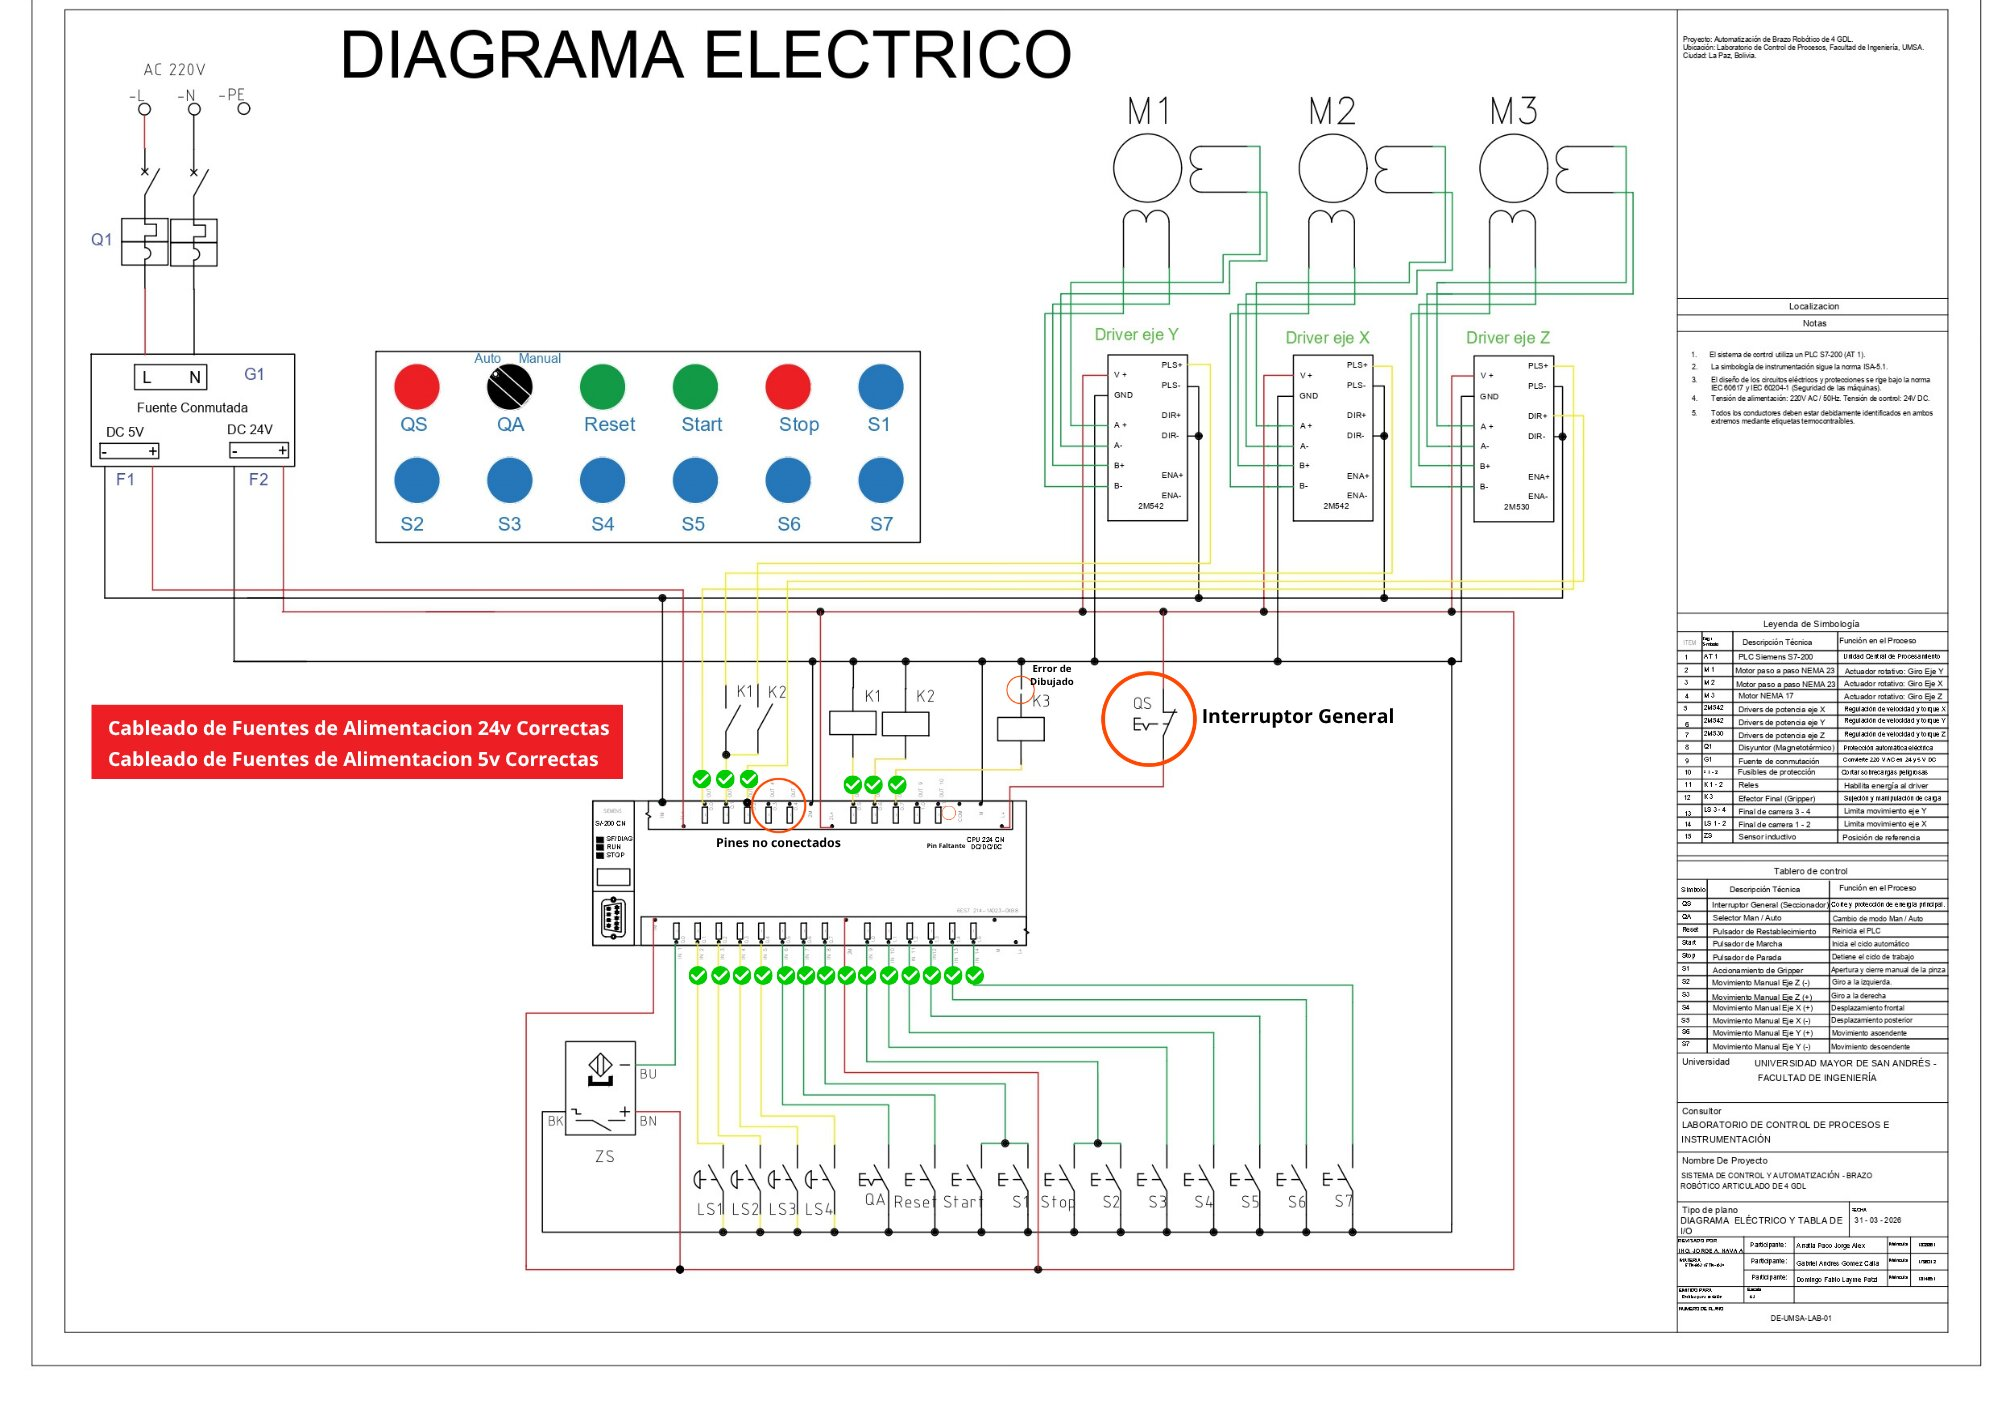
\includegraphics[width=\linewidth]{brazo_electrico_historico_vista.jpg}
\caption{Plano eléctrico heredado (\texttt{planos/electrico/brazo\_electrico\_historico.dwg}). El informe 1 encontró pines sin graficar, DIR+ de X e Y sin conectar y el trazo de la garra equivocado (sección \ref{sec:kaizen}).}
\end{figure}

\section{Etapa de potencia}
\begin{figure}[H]
\centering
\begin{tikzpicture}[node distance=6mm and 9mm]
\node[caja, text width=1.8cm] (red) {red\\220~V AC};
\node[caja, text width=2.6cm, right=of red] (dz) {disyuntor diferencial\\DZ47LE-63\\16~A · 30~mA};
\node[cajan, text width=2.4cm, right=of dz] (f) {fuente conmutada\\24~V / 5~V DC};
\node[caja, text width=2.4cm, right=12mm of f, yshift=14mm] (plc) {PLC CPU 224\\(L+/M 24~V)};
\node[caja, text width=2.4cm, right=12mm of f] (drv) {drivers 2M542 (X, Y)\\y 2M530 (base)\\VDC 24~V};
\node[caja, text width=2.4cm, right=12mm of f, yshift=-14mm] (mando) {sensores, relés\\K1--K3, solenoide};
\draw[flecha] (red) -- (dz); \draw[flecha] (dz) -- (f);
\draw[flecha] (f.east) -- ++(4mm,0) |- (plc.west);
\draw[flecha] (f) -- (drv);
\draw[flecha] (f.east) -- ++(4mm,0) |- (mando.west);
\node[etiq, text width=3.6cm, right=4mm of drv] {los drivers admiten 20--50~V: con 36--48~V el par a alta velocidad mejora (capítulo \ref{cap:drivers})};
\end{tikzpicture}
\caption{Distribución de energía.}
\end{figure}

\section{Etapa de mando}
\begin{figure}[H]
\centering
\begin{tikzpicture}[x=1cm,y=1cm, borne/.style={circle, draw, fill=white, inner sep=1.2pt}, rot/.style={font=\scriptsize\ttfamily, anchor=east}]
% PLC
\draw[thick, fill=naranja!8] (0,0) rectangle (2.4,-10.2);
\node[font=\small\bfseries, align=center] at (1.2,0.45) {PLC S7-200\\CPU 224};
\foreach \y/\t in {-0.6/Q0.0,-1.4/Q0.1,-2.2/Q0.2,-3.0/Q0.3,-3.8/Q0.4,-4.6/Q0.5,-5.4/Q0.6,-6.2/Q0.7}
  {\node[borne] at (2.4,\y) {}; \node[font=\scriptsize\ttfamily, anchor=east] at (2.3,\y) {\t};}
\foreach \y/\t in {-6.9/I0.0,-7.8/I0.1..I0.4,-8.6/I0.5..I0.7,-9.4/I1.0..I1.5}
  {\node[borne] at (0,\y) {}; \node[font=\scriptsize\ttfamily, anchor=west] at (0.1,\y) {\t};}
% relés
\node[draw, fill=gris, minimum width=1.2cm, minimum height=0.8cm, font=\scriptsize] (k1) at (5.2,-4.6) {K1};
\node[draw, fill=gris, minimum width=1.2cm, minimum height=0.8cm, font=\scriptsize] (k2) at (5.2,-5.4) {K2};
\node[draw, fill=gris, minimum width=1.2cm, minimum height=0.8cm, font=\scriptsize] (k3) at (5.2,-6.2) {K3};
\draw[flecha] (2.4,-4.6) -- node[above, etiq]{bobina} (k1); \draw[flecha] (2.4,-5.4) -- (k2); \draw[flecha] (2.4,-6.2) -- (k3);
% drivers
\node[draw, fill=white, minimum width=2.6cm, minimum height=1.5cm, align=center, font=\scriptsize] (dz) at (10.2,-0.9) {\textbf{driver base 2M530}\\PUL \ DIR \ ENA};
\node[draw, fill=white, minimum width=2.6cm, minimum height=1.5cm, align=center, font=\scriptsize] (dx) at (10.2,-2.9) {\textbf{driver X 2M542}\\PUL \ DIR \ ENA};
\node[draw, fill=white, minimum width=2.6cm, minimum height=1.5cm, align=center, font=\scriptsize] (dy) at (10.2,-4.9) {\textbf{driver Y 2M542}\\PUL \ DIR \ ENA};
\draw[thick] (2.4,-0.6) -- (8.9,-0.6) node[pos=0.55, above, etiq]{PUL base};
\draw[thick] (2.4,-2.2) -- (7.6,-2.2) |- (8.9,-1.2) node[pos=0.8, above, etiq]{DIR base};
% Q0.1 por contactos de K1 y K2
\draw[thick] (2.4,-1.4) -- (6.6,-1.4) -- (6.6,-2.6);
\draw[thick] (6.6,-2.6) -- (6.9,-2.6); \draw[thick] (6.9,-2.45) -- (7.2,-2.75); \draw[thick] (7.2,-2.6) -- (8.9,-2.6) node[pos=0.5, above, etiq]{PUL X};
\node[font=\tiny] at (7.05,-2.95) {K1};
\draw[thick] (6.6,-2.6) -- (6.6,-4.6) -- (6.9,-4.6); \draw[thick] (6.9,-4.45) -- (7.2,-4.75); \draw[thick] (7.2,-4.6) -- (8.9,-4.6) node[pos=0.5, above, etiq]{PUL Y};
\node[font=\tiny] at (7.05,-4.95) {K2};
\draw[dashed] (k1.north) -- (7.05,-2.8); \draw[dashed] (k2.north) -- (7.05,-4.8);
\draw[thick] (2.4,-3.0) -- (6.3,-3.0) -- (6.3,-3.2) -- (8.9,-3.2) node[pos=0.6, below, etiq]{DIR X};
\draw[thick] (2.4,-3.8) -- (6.1,-3.8) -- (6.1,-5.2) -- (8.9,-5.2) node[pos=0.8, below, etiq]{DIR Y};
% garra
\node[draw, fill=white, minimum width=2.6cm, minimum height=1cm, align=center, font=\scriptsize] (sol) at (10.2,-6.6) {solenoide de la garra\\24~V DC};
\draw[thick] (k3.east) -- node[above, etiq]{contacto K3, +24~V} (sol.west);
% motores
\node[draw, circle, minimum size=0.9cm, font=\scriptsize, right=6mm of dz] (mz) {M};
\node[draw, circle, minimum size=0.9cm, font=\scriptsize, right=6mm of dx] (mx) {M};
\node[draw, circle, minimum size=0.9cm, font=\scriptsize, right=6mm of dy] (my) {M};
\draw[thick] (dz) -- (mz); \draw[thick] (dx) -- (mx); \draw[thick] (dy) -- (my);
% sensores
\node[draw, fill=white, align=center, font=\scriptsize, text width=3cm, anchor=east] (ind) at (-1.4,-6.75) {inductivo LJ12A3-4-Z/BX\\NPN NA, 3 hilos};
\node[draw, fill=white, align=center, font=\scriptsize, text width=3cm, anchor=east] (fc) at (-1.4,-7.8) {4 finales de carrera};
\node[draw, fill=white, align=center, font=\scriptsize, text width=3cm, anchor=east] (bt) at (-1.4,-9.0) {botonera: selector,\\Stop, Start, S1--S7};
\draw[thick] (ind.east) -- (-0.5,-6.75) -- (-0.5,-6.9) -- (0,-6.9); \draw[thick] (fc) -- (0,-7.8); \draw[thick] (bt.east) -- (-0.7,-9.0) -- (-0.7,-8.6) -- (0,-8.6); \draw[thick] (-0.7,-9.0) -- (-0.7,-9.4) -- (0,-9.4);
\end{tikzpicture}
\caption{Esquema funcional de mando. Q0.1 llega al driver X solo con K1 cerrado y al driver Y solo con K2 cerrado.}
\end{figure}

\nota{\textbf{Este esquema es funcional}: muestra qué señal va a qué componente, verificado con el PLC en marcha. Los bornes exactos, los comunes (1M, 2M, 1L+), el nivel de las entradas PUL/DIR de los drivers (entradas optoacopladas de 5~V, alimentadas desde el riel de 5~V o con resistencias en serie) y la entrada ENA deben tomarse del plano versión 2.0 cuando se termine (guía 2).}

\section{Por qué los relés K1 y K2}
La CPU 224 tiene solo dos generadores de pulsos rápidos, en Q0.0 y Q0.1. Con tres motores, quien diseñó la planta dedicó Q0.0 a la base y repartió Q0.1 entre los dos carros mediante los contactos de K1 y K2. Consecuencias de diseño:
\begin{itemize}
\item X e Y pueden moverse a la vez, pero recibiendo exactamente los mismos pulsos, a la misma frecuencia.
\item Un movimiento con recorridos distintos se divide en un tramo común (K1 y K2 cerrados) y un resto (solo el relé del eje más largo).
\item Un relé tarda unos milisegundos en cerrar: los programas esperan 30--300~ms entre cerrar el relé y dar pulsos, para no perder los primeros.
\item Abrir un relé con el tren en marcha cortaría pulsos a mitad del tramo: los programas solo conmutan los relés con el PTO detenido (SM76.7 = 1).
\end{itemize}

\section{Tensiones medidas}
Mediciones pasivas con multímetro del informe 1 (Lab 1):
\begin{center}\small
\begin{tabular}{@{}lll@{}}
\toprule
\textbf{Punto} & \textbf{Accionado} & \textbf{En reposo}\\
\midrule
entradas de la botonera (I0.4--I1.5) & 21,6~V & 23,1~V\\
salidas de pulsos (multímetro, valor medio) & 0,0--1,2~V & 0,1--0,2~V\\
salidas de dirección & 0,1--5,1~V & 0,1--5,1~V\\
Q0.7 (garra) & 23,2~V & 0,2~V\\
rieles del PLC (1M--1L+, 2M--2L+) & 5,1--23,4~V & 5,2--23,7~V\\
\bottomrule
\end{tabular}
\end{center}
Un multímetro muestra el valor medio de un tren de pulsos, no su forma: para ver la frecuencia hace falta un osciloscopio o un contador (por ejemplo, el contador rápido HSC del propio PLC).

% =====================================================================
\chapter{Motores, drivers, transmisión y frecuencias}\label{cap:drivers}

\section{Cómo se mueve un motor paso a paso}
Un motor paso a paso híbrido de 1,8° tiene 200 posiciones estables por vuelta. El driver alimenta sus dos bobinas (A y B) con corrientes que van girando el campo magnético; con \emph{micropasos}, divide cada paso en partes más pequeñas haciendo las corrientes casi senoidales, lo que da un movimiento más suave.

\begin{figure}[H]
\centering
\begin{tikzpicture}[x=1cm,y=1cm]
\node[cajan, text width=2.4cm] (plc) {PLC\\PUL: un pulso\\DIR: sentido};
\node[caja, text width=3cm, right=10mm of plc] (drv) {driver\\1 pulso = 1 micropaso\\corriente en A y B};
\node[caja, text width=2.4cm, right=10mm of drv] (m) {motor 1,8°\\200 pasos/vuelta};
\node[caja, text width=2.6cm, right=10mm of m] (h) {husillo o\\engranaje};
\draw[flecha] (plc) -- (drv); \draw[flecha] (drv) -- node[above, etiq]{A±, B±} (m); \draw[flecha] (m) -- (h);
\begin{scope}[shift={(1.2,-2.4)}]
\draw[->] (0,0) -- (11.5,0) node[right, etiq]{t};
\node[etiq, anchor=east] at (-0.1,0.9) {$i_A$}; \node[etiq, anchor=east] at (-0.1,-0.9) {$i_B$};
\draw[naranja, thick, domain=0:11, samples=120] plot (\x, {0.8*cos(\x*65)}) ;
\draw[azulg, thick, domain=0:11, samples=120] plot (\x, {0.8*sin(\x*65)});
\node[etiq, text width=6cm] at (5.5,-1.4) {con micropasos, las corrientes de las dos bobinas son casi senoidales y desfasadas 90°};
\end{scope}
\end{tikzpicture}
\caption{Cadena de mando de un eje.}
\end{figure}

\section{Configuración de los drivers}
Los drivers JMC 2M542-N son compatibles con el Leadshine DM542, cuya tabla está en \codigo{global/datasheets/driver\_leadshine\_dm542.pdf}. Los tres drivers del tablero tienen los interruptores en la misma posición (foto del 26/10/2026):

\begin{center}
\begin{tikzpicture}[x=1cm,y=1cm]
\foreach \i/\e in {1/0,2/0,3/1,4/0,5/1,6/1,7/1,8/0} {
  \draw[fill=gris] (\i*0.9,0) rectangle ++(0.6,1.4);
  \ifnum\e=1 \fill[naranja] (\i*0.9+0.08,0.08) rectangle ++(0.44,0.55); \node[font=\tiny\bfseries] at (\i*0.9+0.3,1.2) {ON};
  \else \fill[black!60] (\i*0.9+0.08,0.77) rectangle ++(0.44,0.55); \node[font=\tiny] at (\i*0.9+0.3,0.25) {OFF}; \fi
  \node[font=\scriptsize] at (\i*0.9+0.3,-0.3) {SW\i};
}
\draw[decorate, decoration={brace, mirror, amplitude=4pt}] (0.9,-0.55) -- (3.3,-0.55) node[midway, below=5pt, etiq]{corriente};
\draw[decorate, decoration={brace, mirror, amplitude=4pt}] (3.6,-0.55) -- (4.2,-0.55) node[midway, below=5pt, etiq]{reposo};
\draw[decorate, decoration={brace, mirror, amplitude=4pt}] (4.5,-0.55) -- (7.5,-0.55) node[midway, below=5pt, etiq]{micropasos};
\end{tikzpicture}
\end{center}

\begin{table}[H]
\centering\small
\begin{minipage}[t]{0.47\linewidth}\centering
\begin{tabular}{@{}cccrr@{}}
\toprule
\textbf{SW1} & \textbf{SW2} & \textbf{SW3} & \textbf{pico} & \textbf{RMS}\\
\midrule
ON & ON & ON & 1,00~A & 0,71~A\\
OFF & ON & ON & 1,46~A & 1,04~A\\
ON & OFF & ON & 1,91~A & 1,36~A\\
\rowcolor{naranja!20} OFF & OFF & ON & \textbf{2,37~A} & \textbf{1,69~A}\\
ON & ON & OFF & 2,84~A & 2,03~A\\
OFF & ON & OFF & 3,31~A & 2,36~A\\
ON & OFF & OFF & 3,76~A & 2,69~A\\
OFF & OFF & OFF & 4,20~A & 3,00~A\\
\bottomrule
\end{tabular}
\caption{Corriente de trabajo (SW1--SW3).}
\end{minipage}\hfill
\begin{minipage}[t]{0.5\linewidth}\centering
\begin{tabular}{@{}rcccc@{}}
\toprule
\textbf{pulsos/vuelta} & \textbf{SW5} & \textbf{SW6} & \textbf{SW7} & \textbf{SW8}\\
\midrule
400 & OFF & ON & ON & ON\\
800 & ON & OFF & ON & ON\\
1600 & OFF & OFF & ON & ON\\
3200 & ON & ON & OFF & ON\\
6400 & OFF & ON & OFF & ON\\
12800 & ON & OFF & OFF & ON\\
25600 & OFF & OFF & OFF & ON\\
\rowcolor{naranja!20} \textbf{1000} & ON & ON & ON & OFF\\
2000 & OFF & ON & ON & OFF\\
4000 & ON & OFF & ON & OFF\\
5000 & OFF & OFF & ON & OFF\\
8000 & ON & ON & OFF & OFF\\
10000 & OFF & ON & OFF & OFF\\
20000 & ON & OFF & OFF & OFF\\
25000 & OFF & OFF & OFF & OFF\\
\bottomrule
\end{tabular}
\caption{Micropasos (SW5--SW8).}
\end{minipage}
\end{table}

\begin{itemize}
\item \textbf{SW4 = OFF}: un segundo después del último pulso, la corriente baja a la mitad (el calor baja al 25\,\%, porque $P = I^2R$). Con SW4 = ON se mantiene toda la corriente.
\item \textbf{X e Y deben tener siempre los mismos micropasos}, porque reciben el mismo tren de pulsos: si no, avanzarían distinto con los mismos pulsos.
\end{itemize}

\subsection{Análisis por eje}
\begin{center}\small
\begin{tabularx}{\linewidth}{>{\raggedright}p{2.2cm} >{\raggedright}p{2.6cm} >{\raggedright}p{3cm} >{\raggedright\arraybackslash}X}
\toprule
\textbf{Eje} & \textbf{Motor} & \textbf{Corriente ajustada} & \textbf{Comentario}\\
\midrule
X, Y & NEMA 23, 2,8~A/fase & 1,69~A RMS (2,37~A pico) & 60\,\% de la nominal: el motor trabaja frío pero con menos par (el par es casi proporcional a la corriente)\\
Base & NEMA 17, 1,2~A/fase & desconocida & el 2M530 tiene otra tabla (0,5--3,0~A). Si la posición OFF OFF ON diera más de 1,2~A RMS, el motor se calentaría: \textbf{leer la placa del driver y verificar}\\
\bottomrule
\end{tabularx}
\end{center}

\section{Transmisión y resolución}
\begin{figure}[H]
\centering
\begin{tikzpicture}[node distance=4mm]
\node[cajan] (p) {1 pulso};
\node[caja, right=of p] (m) {$\frac{1}{1000}$ de vuelta del motor};
\node[caja, right=of m] (h) {husillo 5~mm/vuelta (SUPUESTO)};
\node[cajan, right=of h] (r) {0,005~mm del carro};
\draw[flecha] (p) -- (m); \draw[flecha] (m) -- (h); \draw[flecha] (h) -- (r);
\end{tikzpicture}
\caption{Carros X e Y: 200 pulsos por milímetro.}
\end{figure}

\begin{itemize}
\item \textbf{Carros}: $k_{XY} = \dfrac{1000~\text{pulsos/vuelta}}{5~\text{mm/vuelta}} = 200~\text{pulsos/mm}$; resolución 5~µm; recorrido de 170~mm = 34\,000 pulsos.
\item \textbf{Base}: calibrada en la planta midiendo un giro con transportador: $k_\theta = 190{,}3$ pulsos/grado, o sea 68\,508 pulsos por vuelta de la base. Si el driver de la base también da 1000 pulsos por vuelta (SUPUESTO), la reducción mecánica es de unas \textbf{68,5 vueltas del motor por vuelta de la base}. Resolución: 0,0053° por pulso.
\end{itemize}

\section{Frecuencias, velocidades y tiempos}
La velocidad de cada eje sale directamente de la frecuencia del tren de pulsos $f$ (o de su ciclo $T = 1/f$, que es lo que se programa en el PLC):
\[
v_{carro} = \frac{f}{k_{XY}}~[\text{mm/s}], \qquad \omega_{base} = \frac{f}{k_\theta}~[\text{°/s}], \qquad n_{motor} = \frac{60\,f}{1000}~[\text{rpm}] .
\]

\begin{center}\small
\begin{longtable}{>{\raggedright}p{4.6cm} >{\ttfamily}p{1.6cm} r r r}
\toprule
\textbf{Dónde se usa} & \textbf{\rmfamily ciclo} & \textbf{$f$} & \textbf{motor} & \textbf{eje}\\
\midrule
\endhead
jog X/Y, homing X/Y, secuencias, movimientos del gemelo (por defecto) & 250 µs & 4~kHz & 240~rpm & 20~mm/s\\
jog de la base (programa del gemelo), homing de la base, movimientos de la base (por defecto) & 400 µs & 2,5~kHz & 150~rpm & 13,1~°/s\\
jog y secuencias de la base (programa original) & 250 µs & 4~kHz & 240~rpm & 21,0~°/s\\
mínimo admitido por el programa del gemelo (X/Y) & 2000 µs & 500~Hz & 30~rpm & 2,5~mm/s\\
máximo admitido por el programa del gemelo (X/Y) & 200 µs & 5~kHz & 300~rpm & 25~mm/s\\
límite del hardware (PTO de la CPU 224) & 50 µs & 20~kHz & 1200~rpm & 100~mm/s\\
\bottomrule
\end{longtable}
\end{center}

\textbf{Tiempos típicos} a las frecuencias por defecto: recorrer los 170~mm de un carro toma $170/20 = 8{,}5$~s; girar la base 90° toma $90 \times 190{,}3 / 2500 = 6{,}9$~s.

\begin{figure}[H]
\centering
\begin{tikzpicture}[x=0.55cm,y=1cm]
\foreach \i in {0,...,9} {\draw[thick, naranja] (2*\i,0) -- (2*\i,0.8) -- (2*\i+1,0.8) -- (2*\i+1,0) -- (2*\i+2,0);}
\draw[<->] (0,1.05) -- (2,1.05) node[midway, above, etiq]{$T$ = ciclo (SMW68/SMW78, µs)};
\draw[<->] (4,-0.25) -- (5,-0.25) node[midway, below, etiq]{$T/2$};
\draw[decorate, decoration={brace, mirror, amplitude=4pt}] (0,-0.7) -- (20,-0.7) node[midway, below=5pt, etiq]{$N$ pulsos (SMD72/SMD82)};
\node[etiq, anchor=east] at (-0.3,0.4) {Q0.x};
\end{tikzpicture}
\caption{Tren de pulsos del PTO: ancho al 50\,\%, ciclo $T$ y cantidad $N$.}
\end{figure}

\section{Arranque sin rampa y pérdida de pasos}
Un motor paso a paso solo puede arrancar \emph{de golpe} hasta una frecuencia límite (de arranque o \emph{pull-in}), que baja con la carga y la inercia. Por encima de ella, el rotor no alcanza a seguir al campo y pierde pasos: el eje queda atrás de la cuenta del PLC.

Los dos programas del brazo arrancan los trenes a frecuencia constante, sin rampa. Por eso:
\begin{itemize}
\item se trabaja a 2,5--4~kHz, frecuencias que se probaron sin pérdidas visibles;
\item la base del programa del gemelo usa 2,5~kHz (en lugar de 4~kHz) porque arranca más suave;
\item la app limita la velocidad a 500--5000~Hz y recomienda no pasar de 4000~Hz.
\end{itemize}

\section{Recomendaciones}
\begin{enumerate}
\item \textbf{Corriente de X e Y}: subir a 2,84~A pico (ON ON OFF) para aprovechar más el par del NEMA 23 de 2,8~A, vigilando la temperatura.
\item \textbf{SW4 del carro Y}: el husillo de bolas es reversible y el peso del brazo empuja el carro Y. Si el brazo baja solo al quedar quieto, poner SW4 = ON (retención con toda la corriente).
\item \textbf{Rampas}: implementar perfiles de varios segmentos en el PTO (arranque a 1--1,5~kHz, máximo 10--15~kHz, rampa de 0,5--1~s). Así se podría trabajar más rápido sin perder pasos.
\item \textbf{Tensión}: los drivers admiten hasta 50~V; con 36--48~V el par a alta velocidad mejora mucho.
\item \textbf{Base}: verificar el driver 2M530 y el motor de 1,2~A.
\end{enumerate}

% =====================================================================
\chapter{El PLC S7-200: lo necesario para leer los programas}\label{cap:s7200}

\section{El ciclo del PLC}
\begin{figure}[H]
\centering
\begin{tikzpicture}[node distance=8mm]
\node[caja] (a) {leer entradas\\(imagen I)};
\node[cajan, right=of a] (b) {ejecutar OB1\\y subrutinas};
\node[caja, right=of b] (c) {escribir salidas\\(imagen Q)};
\node[caja, right=of c] (d) {comunicación PPI\\y autodiagnóstico};
\draw[flecha] (a) -- (b); \draw[flecha] (b) -- (c); \draw[flecha] (c) -- (d);
\draw[flecha] (d.south) -- ++(0,-5mm) -| (a.south);
\end{tikzpicture}
\caption{Ciclo de barrido. Las peticiones de la PC se atienden en la etapa de comunicación, entre ciclos.}
\end{figure}
El programa se ejecuta de arriba abajo en cada ciclo (unos milisegundos). Las salidas de pulsos (PTO) son la excepción: las genera un circuito de hardware que sigue funcionando aunque el ciclo siga adelante; el programa solo las configura, las arranca y consulta si terminaron.

\section{Áreas de memoria}
\begin{center}\small
\begin{tabularx}{\linewidth}{>{\ttfamily}p{1.4cm} >{\raggedright}p{3.6cm} >{\raggedright\arraybackslash}X}
\toprule
\textbf{\rmfamily Área} & \textbf{Nombre} & \textbf{Uso en el brazo}\\
\midrule
I & imagen de entradas & sensores y botonera (I0.0--I1.5)\\
Q & imagen de salidas & pulsos, direcciones, relés (Q0.0--Q0.7)\\
M & marcas & banderas internas del programa original (M0.0--M10.0)\\
V & memoria de variables & datos y buzón con la PC (VB100, VB104, VB1100--VB1205)\\
SM & memoria especial & configuración y estado del PTO (SMB66--SMD82), SM0.0 (siempre 1), SM0.1 (primer ciclo)\\
T & temporizadores & retardos y vigilancia de tiempos\\
\bottomrule
\end{tabularx}
\end{center}
Tamaños: \codigo{VB} = byte, \codigo{VW} = palabra de 2 bytes (\codigo{VW1102} ocupa VB1102 y VB1103), \codigo{VD} = doble palabra de 4 bytes. El S7-200 guarda los números con el byte más significativo primero (\emph{big-endian}): la app debe leerlos igual.

\section{Temporizadores TON}
La resolución depende del número del temporizador. Esto es clave para leer los programas: \codigo{TON T35, +3} son 30~ms, pero \codigo{TON T38, +2} son 200~ms.

\begin{center}\small
\begin{tabular}{@{}lll@{}}
\toprule
\textbf{Temporizadores TON} & \textbf{Resolución} & \textbf{Ejemplo}\\
\midrule
T32, T96 & 1~ms & --\\
T33--T36, T97--T100 & 10~ms & \codigo{TON T35, +3} = 30~ms\\
T37--T63, T101--T255 & 100~ms & \codigo{TON T58, +120} = 12~s\\
\bottomrule
\end{tabular}
\end{center}

\section{Salidas de pulsos (PTO)}\label{sec:pto}
\begin{center}\small
\begin{tabular}{@{}lll@{}}
\toprule
\textbf{PTO0 (Q0.0)} & \textbf{PTO1 (Q0.1)} & \textbf{Función}\\
\midrule
SMB66 & SMB76 & estado (SM66.7 / SM76.7 = 1: en reposo)\\
SMB67 & SMB77 & byte de control\\
SMW68 & SMW78 & ciclo en µs o ms\\
SMD72 & SMD82 & cantidad de pulsos\\
\bottomrule
\end{tabular}
\end{center}

\begin{figure}[H]
\centering
\begin{tikzpicture}[x=1.45cm,y=1cm]
\foreach \b/\v/\t in {7/1/{habilitar\\PTO/PWM}, 6/0/{0 = PTO\\1 = PWM}, 5/0/{0 = un\\segmento}, 4/0/{(PWM)}, 3/0/{base de\\tiempo µs}, 2/1/{actualizar\\cantidad}, 1/0/{(PWM)}, 0/1/{actualizar\\ciclo}} {
  \ifnum\v=1 \def\col{naranja!25}\else\def\col{gris}\fi \draw[fill=\col] (7-\b,0) rectangle ++(1,0.8);
  \node[font=\small\bfseries] at (7.5-\b,0.4) {\v};
  \node[font=\scriptsize\ttfamily] at (7.5-\b,1.05) {SM77.\b};
  \node[font=\tiny, align=center] at (7.5-\b,-0.45) {\t};
}
\node[font=\small, anchor=west] at (8.2,0.4) {= \codigo{16\#85}};
\end{tikzpicture}
\caption{Byte de control \texttt{16\#85} que usan los dos programas: PTO de un solo segmento, base de tiempo en µs, con actualización de ciclo y cantidad.}
\end{figure}

Para arrancar un tren se escriben el control, el ciclo y la cantidad, y se ejecuta \codigo{PLS}. Para detenerlo antes de tiempo, \codigo{SMB77 = 0} y \codigo{PLS 1}. Con un solo segmento, el ciclo es constante durante todo el tren (sin rampa).

\section{Instrucciones que aparecen en los programas}
\begin{center}\small
\begin{longtable}{>{\ttfamily}p{3.3cm} >{\raggedright\arraybackslash}p{11.8cm}}
\toprule
\textbf{\rmfamily Instrucción (AWL)} & \textbf{Qué hace}\\
\midrule
\endhead
LD / LDN & empieza un camino con un contacto abierto / cerrado\\
A / AN & contacto en serie (Y) abierto / cerrado\\
O / ON & contacto en paralelo (O) abierto / cerrado\\
EU / ED & detecta el flanco ascendente / descendente: deja pasar la corriente un solo ciclo\\
= & bobina: copia el resultado lógico en un bit\\
S bit, n / R bit, n & pone a 1 / a 0 \emph{n} bits a partir de \emph{bit}, y quedan así\\
LPS / LRD / LPP & guardan, leen y sacan el resultado lógico de una pila: así AWL representa las ramificaciones de un segmento ladder\\
ALD / OLD & combinan en serie / en paralelo dos bloques de contactos\\
LDW= , AW<> , AD> \dots & contactos de comparación de palabras (W), dobles palabras (D) o bytes (B)\\
MOVB / MOVW / MOVD & copian un byte, una palabra o una doble palabra\\
+D , -D & suma y resta de dobles palabras con signo\\
FILL & llena un bloque de palabras con un valor\\
TON T, PT & temporizador con retardo a la conexión: se activa cuando la entrada lleva PT unidades en 1\\
PLS 0 / PLS 1 & aplica la configuración y arranca (o detiene) el PTO0 / PTO1\\
CALL SBRn / CRET & llama a una subrutina / vuelve de ella\\
\bottomrule
\end{longtable}
\end{center}

\section{Cómo se lee un diagrama ladder}
\begin{center}
\begin{tikzpicture}[x=1cm,y=1cm]
\foreach \x/\p/\t in {0.8/na/contacto abierto: pasa si el bit es 1, 4.6/nc/contacto cerrado: pasa si el bit es 0, 8.4/pf/flanco positivo: pasa un solo ciclo}
  {\draw[ld] (\x-0.5,0) -- (\x+0.5,0); \pic at (\x,0) {\p={bit}}; \node[etiq, text width=3.3cm] at (\x,-0.8) {\t};}
\draw[ld] (11.6,0) -- (12.6,0); \pic at (12.1,0) {bob={bit}{}{}}; \node[etiq, text width=2.4cm] at (12.1,-0.8) {bobina: escribe el bit};
\draw[ld] (0.3,-2.5) -- (1.3,-2.5); \pic at (0.8,-2.5) {bob={bit}{S}{1}}; \node[etiq, text width=3cm] at (0.8,-3.4) {pone a 1 (set) y queda};
\draw[ld] (4.1,-2.5) -- (5.1,-2.5); \pic at (4.6,-2.5) {bob={bit}{R}{1}}; \node[etiq, text width=3cm] at (4.6,-3.4) {pone a 0 (reset)};
\draw[ld] (7.4,-2.5) -- (7.9,-2.5); \pic at (8.4,-2.5) {cmp={VW320}{==I}{11}}; \draw[ld] (7.9,-2.5)--(8.9,-2.5); \node[etiq, text width=3.3cm] at (8.4,-3.4) {comparación: pasa si VW320 = 11};
\draw[ld] (10.9,-2.5) -- (11.4,-2.5); \node[fb] at (11.4,-2.5) {\textbf{MOV\_W}\\IN \ +20\\OUT VW320}; \node[etiq, text width=3cm] at (12.3,-3.45) {cuadro: copia, suma, temporiza\dots};
\end{tikzpicture}
\end{center}

\section{Máquinas de pasos}
Las secuencias de los dos programas se escriben como \textbf{máquinas de pasos}: una palabra guarda el número de paso (VW320 o VW322 en el programa original, VW1136 en el del gemelo). Cada segmento pregunta «¿estoy en el paso N?», hace su tarea y, cuando se cumple la condición de salida, escribe el número del paso siguiente. Se dibujan como diagramas de estados, y su comportamiento puede modelarse con redes de Petri (sección \ref{sec:petri}).

% =====================================================================
\chapter{Programa original de secuencias}\label{cap:original}

\section{Origen y estructura}
Es el programa que tenía cargado el PLC al empezar el proyecto: una versión del programa de Miguel («BRAZO MIGUEL ROBADO»), con un pequeño buzón en VB100/VB104 para recibir órdenes de la PC. Se subió desde el PLC el 26/10/2026 y está en el repositorio como \codigo{programas-plc/brazo\_secuencias\_original\_v1.awl} (y \codigo{.mwp}); el listado completo está en el apéndice \ref{ap:original}.

\begin{figure}[H]
\centering
\begin{tikzpicture}[node distance=6mm and 8mm]
\node[cajan, text width=3.8cm] (ob1) {\textbf{OB1} (10 segmentos)\\arranque, paro, emergencia, selección de modo, estado};
\node[caja, text width=3cm, right=16mm of ob1, yshift=14mm] (man) {\textbf{SBR20 MANUAL}\\(9 segmentos)\\jog y garra};
\node[caja, text width=3cm, right=16mm of ob1, yshift=-14mm] (aut) {\textbf{SBR21 AUTO}\\(37 segmentos)\\secuencias 1 y 2};
\node[caja, text width=3cm, right=10mm of aut] (hom) {\textbf{SBR0 HOMING}\\(9 segmentos)\\X, base, Y};
\draw[flecha] (ob1) -- node[above, etiq, sloped]{I0.5 = 0} (man);
\draw[flecha] (ob1) -- node[below, etiq, sloped]{I0.5 = 1} (aut);
\draw[flecha] (aut) -- node[above, etiq]{sin referencia} (hom);
\end{tikzpicture}
\caption{Estructura del programa original.}
\end{figure}

\section{Memoria que usa}
\begin{center}\small
\begin{longtable}{>{\ttfamily}p{2.4cm} >{\raggedright\arraybackslash}p{12.6cm}}
\toprule
\textbf{\rmfamily Dirección} & \textbf{Significado}\\
\midrule
\endhead
\multicolumn{2}{@{}l}{\textbf{Órdenes de la PC} (las escribe la app con el perfil \emph{cargado})}\\
V104.0 & iniciar (equivale a I0.7)\\
V104.1 & paro en automático\\
V104.2 & emergencia (queda enclavada)\\
V104.3 / V104.4 & forzar modo (con VB104 = 0, el modo lo decide I0.5)\\
V104.5 / V104.6 & paro / emergencia adicionales\\
V104.7 & latido: la PC lo alterna; si no cambia en 5~s, el PLC borra VB104\\
V100.0 / V100.2 / V100.3 & iniciar / paro / rearmar por flanco\\
\multicolumn{2}{@{}l}{\textbf{Marcas internas}}\\
M4.0 & inicio pedido (I0.7 o V104.0, sin emergencia)\\
M5.0 & flanco del inicio: dura un ciclo\\
M4.3 & modo automático (I0.5 = 1)\\
M4.5 & paro (I0.6 o V104.5)\\
M4.6 / M4.7 & emergencia / emergencia enclavada\\
M5.1 & flanco de rearme (V100.3)\\
M5.3 & flanco del latido\\
M5.5 / M5.6 & flancos de I0.2 / I0.4 (final opuesto pisado durante el homing)\\
M0.0 / M0.5 & homing permitido / homing pedido\\
M0.3 & \textbf{referenciado}\\
M5.2 & falla de homing\\
M1.0 & inicio pedido desde la PC (V100.0) en automático\\
M1.1 & final de carrera cortó el carro X en automático\\
M10.0 & auxiliar para alternar la garra\\
\multicolumn{2}{@{}l}{\textbf{Estado para la PC}}\\
V200.0 / .1 / .3 / .7 & listo / ocupado / falla de homing / referenciado\\
V301.0 -- V301.6 & homing en curso, listo, secuencia 1 en curso y terminada, secuencia 2 en curso y terminada, Y arriba en la secuencia 2\\
V302.0 & la próxima secuencia es la 2\\
VW320 / VW322 & paso de la secuencia automática / del homing\\
VB201 -- VB203 & copia de los pasos y de IB0\\
\multicolumn{2}{@{}l}{\textbf{Constantes} (se cargan en el primer ciclo)}\\
VD330 / VD334 & avance de X en las secuencias: 20\,000 / 14\,000 pulsos\\
VD340 / VD344 / VD348 & pulsos máximos de búsqueda del homing: X 30\,000, Y 25\,000, base 45\,000\\
\bottomrule
\end{longtable}
\end{center}
La app reconoce este programa por la firma VD340 = 30\,000 y VD344 = 25\,000.

\section{Bloque principal OB1}
\begin{center}\small
\begin{longtable}{>{\raggedright}p{1.2cm} >{\raggedright\arraybackslash}p{13.8cm}}
\toprule
\textbf{Seg.} & \textbf{Qué hace}\\
\midrule
\endhead
1 & Señales de mando: borra VB104 en el primer ciclo; vigila el latido V104.7 con T61 (5~s); calcula inicio (M4.0) y su flanco (M5.0), modo automático (M4.3), paro (M4.5), emergencia (M4.6) y la enclava (M4.7); flancos de rearme (M5.1) y de los finales opuestos (M5.5, M5.6).\\
2 & Emergencia: corta los dos PTO (SMB67/77 = 0 y PLS), apaga Q0.0--Q0.6, borra los pasos y las banderas. Rearme: con la emergencia ya liberada, un inicio (M5.0) o V100.3 quitan el enclavamiento.\\
3 & Primer ciclo (SM0.1): apaga las salidas, borra marcas y memoria de mando y estado, y carga las constantes VD330--VD348.\\
4 & Paro en automático: flanco de I0.6, V300.2, \textbf{I1.0} o V104.1, con el selector en automático. Corta los trenes, apaga salidas y vuelve las secuencias al inicio.\\
5 & Al pasar a manual: corta todo y reinicia; en manual y sin emergencia llama a SBR20.\\
6 & Al pasar a automático: corta todo y permite el homing; en automático y sin emergencia llama a SBR21.\\
7 & Flanco de V100.0 en automático: inicio desde la PC (M1.0). Flanco de V100.2: paro desde la PC (V300.2).\\
8 & Publica el estado en VB200--VB203.\\
9 & Protección en automático: si X avanza y pisa I0.2, o retrocede y pisa I0.1, corta el PTO1 (M1.1).\\
10 & Copia VD210/VD220 en VD304/VD308 (posiciones; en este programa siempre son 0).\\
\bottomrule
\end{longtable}
\end{center}

\begin{figure}[H]
\centering
\begin{tikzpicture}[x=1cm,y=1cm]
\draw[barra] (0,0.6) -- (0,-2.4);
\draw[ld] (0,0) -- (8,0); \draw[ld] (0.4,0) -- (0.4,-1) -- (2.2,-1) -- (2.2,0);
\pic at (1.3,0) {na={I0.7}}; \pic at (1.3,-1) {na={V104.0}};
\pic at (3.4,0) {nc={V104.2}}; \pic at (5,0) {nc={V104.6}}; \pic at (7.2,0) {bob={M4.0}{}{}};
\node[etiq, text width=3cm, anchor=west] at (8.2,0) {inicio pedido\\(panel o PC)};
\draw[ld] (0,-1.9) -- (5.6,-1.9);
\pic at (1.3,-1.9) {na={M4.0}}; \pic at (3,-1.9) {pf={}}; \pic at (4.8,-1.9) {bob={M5.0}{}{}};
\node[etiq, text width=3.6cm, anchor=west] at (5.8,-1.9) {un solo ciclo: arranca homing o secuencia};
\end{tikzpicture}
\caption{OB1, segmento 1 (parte): inicio por I0.7 \emph{o} V104.0, sin emergencia.}
\end{figure}

\begin{figure}[H]
\centering
\begin{tikzpicture}[x=1cm,y=1cm]
\draw[barra] (0,0.6) -- (0,-1.6);
\draw[ld] (0,0) -- (9.4,0);
\draw[ld] (0.3,0) -- (0.3,-1) -- (2.9,-1) -- (2.9,0);
\pic at (0.9,0) {na={I0.2}}; \pic at (2.1,0) {nc={Q0.3}};
\pic at (0.9,-1) {na={I0.1}}; \pic at (2.1,-1) {na={Q0.3}};
\pic at (3.8,0) {na={M4.3}}; \pic at (5,0) {na={Q0.5}}; \pic at (6.2,0) {nc={SM76.7}};
\node[fb] at (7,0) {SMB77 = 0, \textbf{PLS} 1};
\pic at (10.3,0) {bob={M1.1}{S}{1}}; \draw[ld] (9.4,0) -- (10.8,0);
\end{tikzpicture}
\caption{OB1, segmento 9: en automático, el carro X se detiene si llega al final del lado hacia el que avanza.}
\end{figure}

\section{Modo manual (SBR20)}
\begin{center}\small
\begin{longtable}{>{\raggedright}p{1.2cm} >{\raggedright\arraybackslash}p{13.8cm}}
\toprule
\textbf{Seg.} & \textbf{Qué hace}\\
\midrule
\endhead
1 & Con cada flanco de inicio (I0.7) alterna la garra Q0.7 (abre si estaba cerrada, cierra si estaba abierta).\\
2, 3 & I1.0 (o I1.1), con el PTO0 libre: DIR base Q0.2 = 0 (o 1) y paquete de 100 pulsos a 4~kHz.\\
4 & Al soltar los dos pulsadores de la base: corta el PTO0.\\
5, 6 & I1.2 / I1.3 sin el pulsador contrario, sin el final del lado de avance y con K2 abierto: cierra K1, fija DIR X y, tras 30~ms (T35/T36), da paquetes de 100 pulsos a 4~kHz.\\
7, 8 & Igual para Y con I1.4 / I1.5, K2 y T97/T98 (exige K1 abierto).\\
9 & Sin ningún pulsador de X/Y: corta el PTO1 y, 30~ms después (T99), abre K1 y K2.\\
\bottomrule
\end{longtable}
\end{center}

\begin{figure}[H]
\centering
\begin{tikzpicture}[x=1cm,y=1cm]
\draw[barra] (0,0.6) -- (0,-4.4);
\draw[ld] (0,0) -- (8.4,0);
\pic at (0.9,0) {na={I1.2}}; \pic at (2.3,0) {nc={I1.3}}; \pic at (3.7,0) {nc={I0.2}}; \pic at (5.1,0) {nc={Q0.6}};
\pic at (6.4,0) {bob={Q0.5}{S}{1}};
\draw[ld] (5.7,0) -- (5.7,-1.2) -- (8.4,-1.2); \pic at (6.4,-1.2) {bob={Q0.3}{R}{1}};
\draw[ld] (5.7,-1.2) -- (5.7,-2.3) -- (6.2,-2.3); \node[fb] at (6.2,-2.3) {\textbf{TON} T35, PT 3 (30 ms)};
\node[etiq, text width=3.4cm, anchor=west] at (8.6,-0.5) {cierra K1 (driver X) y pone DIR X adelante};
\draw[ld] (0,-3.7) -- (7.1,-3.7);
\pic at (0.9,-3.7) {na={T35}}; \pic at (2.3,-3.7) {na={I1.2}}; \pic at (3.7,-3.7) {nc={I0.2}}; \pic at (5.1,-3.7) {na={SM76.7}};
\node[fb] at (6.1,-3.7) {\textbf{PTO1}: SMB77 = 16\#85\\SMW78 = 250 µs\\SMD82 = 100\\\textbf{PLS} 1};
\end{tikzpicture}
\caption{SBR20, segmento 5: jog de X adelante.}
\end{figure}

\nota{Como el paquete se corta al soltar el pulsador (segmento 9), no se sabe cuántos de los 100 pulsos salieron: con este programa la posición no se puede contar con exactitud. El programa del gemelo corrige esto dejando terminar cada paquete.}

\section{Homing (SBR0)}
\begin{center}\small
\begin{longtable}{>{\raggedright}p{1.2cm} >{\raggedright\arraybackslash}p{13.8cm}}
\toprule
\textbf{Seg.} & \textbf{Qué hace}\\
\midrule
\endhead
1 & Homing permitido (M0.0), pedido (M0.5), sin falla y en reposo: marca «homing en curso» y va al paso 10.\\
2 & Paso 10: abre K2, cierra K1, DIR X atrás (Q0.3 = 1); a los 50~ms (T34) pasa al 11.\\
3 & Paso 11: arranca el PTO1 con VD340 = 30\,000 pulsos a 4~kHz; al llegar a I0.1 lo corta, abre K1 y pasa al 20.\\
4 & Paso 20: DIR base hacia el inductivo (Q0.2 = 1) y PTO0 con VD348 = 45\,000 pulsos a 2,5~kHz; al llegar a I0.0 lo corta y pasa al 30.\\
5 & Paso 30: abre K1, cierra K2, DIR Y abajo (Q0.4 = 1); a los 50~ms (T33) pasa al 31.\\
6 & Paso 31: PTO1 con VD344 = 25\,000 pulsos; al llegar a I0.3 lo corta, abre K2 y pasa al 40.\\
7 & Paso 40: abre la garra; a los 400~ms (T37) pasa al 50.\\
8 & Paso 50: pone las posiciones en cero, marca \textbf{referenciado} (M0.3) y homing terminado.\\
9 & Fallas: tiempo excedido (T58 = 12~s en X, T59 = 25~s en la base, T60 = 12~s en Y), tren terminado sin sensor, o final opuesto pisado (M5.5, M5.6). Corta todo y marca M5.2.\\
\bottomrule
\end{longtable}
\end{center}

\begin{figure}[H]
\centering
\begin{tikzpicture}[node distance=5mm and 7mm]
\node[estado] (s10) {\textbf{10}\\K1, X atrás};
\node[estado, right=of s10] (s11) {\textbf{11}\\PTO1 30000 p\\a 4 kHz};
\node[estado, right=of s11] (s20) {\textbf{20}\\PTO0 45000 p\\a 2,5 kHz};
\node[estado, right=of s20] (s30) {\textbf{30}\\K2, Y abajo};
\node[estado, below=of s30] (s31) {\textbf{31}\\PTO1 25000 p};
\node[estado, left=of s31] (s40) {\textbf{40}\\abre garra};
\node[estadon, left=of s40] (s50) {\textbf{50}\\ceros,\\referenciado};
\node[estado, left=of s50, fill=rojo!10, draw=rojo] (f) {\textbf{falla}\\M5.2};
\draw[flecha] (s10) -- node[trans, above=1mm]{50 ms} (s11);
\draw[flecha] (s11) -- node[trans, above=1mm]{I0.1} (s20);
\draw[flecha] (s20) -- node[trans, above=1mm]{I0.0} (s30);
\draw[flecha] (s30) -- node[trans, right]{50 ms} (s31);
\draw[flecha] (s31) -- node[trans, above=1mm]{I0.3} (s40);
\draw[flecha] (s40) -- node[trans, above=1mm]{400 ms} (s50);
\draw[flecha, rojo, dashed] (s11.south) .. controls +(0,-1.6) and +(0.6,0.6) .. node[trans, pos=0.3, right]{12 s, sin sensor} (f.north east);
\end{tikzpicture}
\caption{Máquina de pasos del homing (VW322).}
\end{figure}

\begin{figure}[H]
\centering
\begin{tikzpicture}[x=1cm,y=1cm]
\draw[barra] (0,0.6) -- (0,-2.6);
\draw[ld] (0,0) -- (3,0); \pic at (1,0) {cmp={VW322}{==I}{11}}; \pic at (2.2,0) {pf={}};
\node[fb] at (3,0) {\textbf{PTO1}: SMB77 = 16\#85, SMW78 = 250 µs\\SMD82 = VD340 (30000), \textbf{PLS} 1};
\draw[ld] (0,-1.7) -- (7.5,-1.7); \pic at (1,-1.7) {cmp={VW322}{==I}{11}}; \pic at (2.5,-1.7) {na={I0.1}};
\node[fb] at (3.2,-1.7) {SMB77 = 0, \textbf{PLS} 1\\(corta el tren)};
\pic at (6.4,-1.7) {bob={Q0.5}{R}{1}};
\draw[ld] (7.5,-1.7) -- (7.9,-1.7); \node[fb] at (7.9,-1.7) {\textbf{MOV\_W} +20 $\rightarrow$ VW322};
\end{tikzpicture}
\caption{SBR0, segmento 3: arranca el tren hacia atrás y lo corta al llegar a I0.1.}
\end{figure}

\section{Secuencias automáticas (SBR21)}
Sin referencia, el primer inicio ejecuta el homing (segmento 1). Con referencia, el primer inicio ejecuta la \textbf{secuencia 1} y los siguientes la \textbf{secuencia 2} (V302.0 queda en 1).

\begin{center}\small
\begin{longtable}{>{\raggedright}p{1.6cm} >{\raggedright}p{1.2cm} >{\raggedright}p{6.2cm} >{\raggedright\arraybackslash}p{5.4cm}}
\toprule
\textbf{Pasos} & \textbf{Seg.} & \textbf{Movimiento} & \textbf{Pulsos / tiempo}\\
\midrule
\endhead
\multicolumn{4}{@{}l}{\textbf{Secuencia 1}}\\
10--12 & 3--5 & Y sube (K2, Q0.4 = 0) & 12\,000 (60~mm), relé 200~ms\\
20--21 & 6--7 & base gira (Q0.2 = 0) & 17\,000 ($\approx$89°)\\
30--32 & 8--10 & X avanza (K1, Q0.3 = 0) & VD330 = 20\,000 (100~mm)\\
40 & 11 & abre la garra; fin & --\\
\multicolumn{4}{@{}l}{\textbf{Secuencia 2}}\\
100 & 13 & cierra la garra (toma la pieza) & 400~ms\\
110--112 & 14--16 & Y sube & 5\,000 (25~mm)\\
120--122 & 17--19 & X retrocede (Q0.3 = 1) & VD334 = 14\,000 (70~mm)\\
130--131 & 20--21 & base gira (Q0.2 = 0) & 18\,000 ($\approx$95°)\\
140--142 & 22--24 & Y baja (Q0.4 = 1) & 14\,000 (70~mm)\\
150 & 25 & abre la garra (deja la pieza) & 400~ms\\
160--162 & 26--28 & Y sube & 14\,000\\
170--171 & 29--30 & base vuelve (Q0.2 = 1) & 18\,000\\
180--182 & 31--33 & X avanza & 14\,000\\
190--192 & 34--36 & Y baja & 5\,000\\
200 & 37 & abre la garra; fin & --\\
\bottomrule
\end{longtable}
\end{center}
Patrón de cada movimiento: (1) cerrar el relé y fijar la dirección, esperar 200~ms (T38, T40\dots{}); (2) arrancar el tren de pulsos a 4~kHz; (3) esperar 100~ms y luego a que SM76.7 (o SM66.7) indique que terminó.

\section{Limitaciones}
\begin{itemize}
\item No conoce la posición: solo sabe si hizo el homing.
\item Solo hace dos rutinas fijas; para cambiarlas hay que reprogramar el PLC.
\item El jog corta los paquetes al soltar: no se puede contar con exactitud.
\item Los finales de carrera solo se vigilan en el homing, en el jog y (para X) en automático.
\item Con este programa, la app \emph{estima} la posición (sección \ref{sec:estimador}).
\end{itemize}

% =====================================================================
\chapter{Programa del gemelo: \texttt{brazo\_gemelo}}\label{cap:gemeloplc}

\section{Por qué un programa nuevo}
El programa original no podía ser la «mitad física» de un gemelo digital: no guarda la posición y solo sabe hacer dos rutinas. El programa \codigo{gemelo-digital/plc/brazo\_gemelo.awl} (proyecto \codigo{.mwp} al lado; listado completo en el apéndice \ref{ap:gemelo}) se escribió conservando el modo manual y el homing del programa de Miguel, y agregando:
\begin{enumerate}
\item \textbf{cuenta de pulsos} de cada eje, con signo: la posición es exacta mientras no se pierdan pasos;
\item \textbf{finales de carrera que cortan} cualquier tren de pulsos y fijan la posición;
\item un \textbf{buzón de órdenes} en la memoria V para que la PC pida homing, movimientos libres, garra, paro y velocidad;
\item un \textbf{watchdog}: si la PC deja de dar señales de vida durante un movimiento, el PLC se detiene.
\end{enumerate}
Compiló sin errores en STEP 7-Micro/WIN (CPU 224 CN) y está cargado en el PLC desde el 27/10/2026. Su bloque de sistema dejó el puerto en la dirección PPI 2 a 9,6~kbit/s.

\begin{figure}[H]
\centering
\begin{tikzpicture}[node distance=5mm and 8mm]
\node[cajan, text width=4cm] (ob1) {\textbf{OB1} (13 segmentos)\\primer ciclo, firma, paro,\\finales de carrera, cuenta,\\selección de modo, estado};
\node[caja, text width=3.2cm, right=14mm of ob1, yshift=13mm] (man) {\textbf{SBR3 MANUAL}\\(21 segmentos)\\jog con cuenta exacta};
\node[caja, text width=3.2cm, right=14mm of ob1, yshift=-13mm] (rem) {\textbf{SBR4 REMOTO}\\(64 segmentos)\\buzón, movimientos,\\homing, watchdog};
\node[caja, text width=2.5cm, right=8mm of man] (pb) {\textbf{SBR1}\\pulsos base};
\node[caja, text width=2.5cm, right=8mm of rem] (pxy) {\textbf{SBR2}\\pulsos X/Y};
\node[caja, text width=2.5cm, below=6mm of ob1] (paro) {\textbf{SBR0 PARO}};
\draw[flecha] (ob1) -- node[above, etiq, sloped]{I0.5 = 0} (man);
\draw[flecha] (ob1) -- node[below, etiq, sloped]{I0.5 = 1} (rem);
\draw[flecha] (man) -- (pb); \draw[flecha] (rem) -- (pxy);
\draw[flecha] (man.south east) -- (pxy.north west); \draw[flecha] (rem.north east) -- (pb.south west);
\draw[flecha] (ob1) -- (paro);
\end{tikzpicture}
\caption{Estructura de \texttt{brazo\_gemelo}. SBR1 y SBR2 son los únicos lugares donde se arrancan trenes de pulsos: así toda la cuenta pasa por un solo sitio.}
\end{figure}

\section{Mapa de memoria}
\begin{center}\small
\begin{longtable}{>{\ttfamily}p{3cm} >{\raggedright}p{1.2cm} >{\raggedright\arraybackslash}p{10.8cm}}
\toprule
\textbf{\rmfamily Dirección} & \textbf{Quién} & \textbf{Contenido}\\
\midrule
\endhead
\multicolumn{3}{@{}l}{\textbf{Buzón de órdenes} (lo escribe la PC en una sola escritura de 20 bytes)}\\
VB1100 & PC & orden: 1 homing, 2 mover, 3 paro, 4 cerrar garra, 5 abrir garra\\
VB1101 & PC & secuencia: el PLC ejecuta cuando cambia\\
VW1102 & PC & latido (watchdog de 2~s)\\
VD1104 / 1108 / 1112 & PC & pulsos relativos de base / X / Y, con signo\\
VW1116 / VW1118 & PC & ciclo del tren X/Y (200--2000~µs) y de la base (250--4000~µs)\\
\multicolumn{3}{@{}l}{\textbf{Estado} (lo lee la PC: 40 bytes desde VB1120)}\\
VB1120 & PLC & estado: 0 reposo, 1 homing, 2 moviendo\\
VB1121 & PLC & eco de la secuencia\\
VB1122 & PLC & .0 referenciado, .1 remoto (I0.5), .2 PTO0 ocupado, .3 PTO1 ocupado, .4 posición incierta, .5 watchdog\\
VB1123 & PLC & error: 1 ocupado, 2 fuera de recorrido, 3 watchdog, 4 sin homing, 5 orden desconocida, 6 paro\\
VD1124 / 1128 / 1132 & PLC & posición de base / X / Y en pulsos\\
VW1136 & PLC & paso de la máquina de estados\\
VB1138 / 1139 / 1140 & PLC & copia de IB0, IB1 y QB0\\
VB1141 & PLC & firma \codigo{16\#47}\\
VD1144 / 1148 / 1152 & PLC & tramo en curso de base / X / Y\\
VW1156 / VW1158 & PLC & ciclo en curso X/Y / base\\
\multicolumn{3}{@{}l}{\textbf{Uso interno}}\\
VW1160 & & último latido visto\\
VB1162 & & orden que se está ejecutando\\
VD1164 / 1168 / 1172 & & destino de X / Y / base\\
VD1176 / 1180 / 1184 & & $|\Delta X|$, $|\Delta Y|$, $|\Delta\theta|$\\
VD1188 / VD1192 & & tramo común / resto\\
VW1196 / VW1198, VD1202 & & parámetros para SBR2 / SBR1: ciclo y pulsos\\
V1200.0 / .1 & & tramo de la base / de X-Y pendiente de sumar\\
V1200.2 / .3 & & posición incierta / referenciado\\
V1200.5 / .6 / .7 & & watchdog / orden de la PC en curso / orden nueva por validar\\
V1201.0 & & tramo de X-Y recién arrancado\\
\bottomrule
\end{longtable}
\end{center}

\section{Bloque principal OB1}
\begin{center}\small
\begin{longtable}{>{\raggedright}p{1.2cm} >{\raggedright\arraybackslash}p{13.8cm}}
\toprule
\textbf{Seg.} & \textbf{Qué hace}\\
\midrule
\endhead
1 & Primer ciclo: apaga Q0.0--Q0.7 y los PTO, llena VB1100--VB1209 con ceros y carga ciclos por defecto (250~µs X/Y, 400~µs base).\\
2 & Escribe la firma \codigo{16\#47} en VB1141 en cada ciclo.\\
3 & Paro: flanco de I0.6 o cualquier cambio del selector I0.5; error 6 y llamada a PARO.\\
4 & X yendo hacia atrás (K1, DIR = 1) con el tren en marcha y llega a I0.1: corta el PTO1, anula el tramo y fija X = 0. Si K2 también estaba cerrado, marca posición incierta (Y pudo quedar a medio tramo).\\
5 & Igual con I0.2: X = 34\,000.\\
6 & Igual con I0.3: Y = 0.\\
7 & Igual con I0.4: Y = 34\,000.\\
8 & Al terminar un tramo de la base (flanco de SM66.7): suma el tramo a VD1124.\\
9 & Al terminar un tramo de Q0.1 (flanco de SM76.7): suma los tramos a X (VD1128) y a Y (VD1132).\\
10 & Selector en manual: llama a MANUAL (SBR3).\\
11 & Selector en automático: llama a REMOTO (SBR4).\\
12 & Copia IB0, IB1 y QB0 en VB1138--VB1140 para la PC.\\
13 & Banderas de estado en VB1122.\\
\bottomrule
\end{longtable}
\end{center}

\begin{figure}[H]
\centering
\begin{tikzpicture}[x=1cm,y=1cm]
\draw[barra] (0,0.6) -- (0,-1.6);
\draw[ld] (0,0) -- (5.6,0);
\pic at (0.9,0) {na={I0.1}}; \pic at (2.2,0) {na={Q0.5}}; \pic at (3.5,0) {na={Q0.3}}; \pic at (4.8,0) {nc={SM76.7}};
\node[fb] at (5.6,0) {SMB77 = 0, \textbf{PLS} 1 (corta)\\R V1200.1 (tramo anulado)\\\textbf{MOV\_DW} 0 $\rightarrow$ VD1128 (X = 0)};
\node[etiq, text width=4.8cm, anchor=west] at (0.4,-1.1) {X yendo hacia atrás (K1 cerrado, DIR = 1) con el tren en marcha y llega al final I0.1};
\end{tikzpicture}
\caption{OB1, segmento 4: el final de carrera corta el tren y fija la posición exacta.}
\end{figure}

\begin{figure}[H]
\centering
\begin{tikzpicture}[x=1cm,y=1cm]
\draw[barra] (0,0.6) -- (0,-1.8);
\draw[ld] (0,0) -- (4.2,0);
\pic at (1,0) {na={SM76.7}}; \pic at (2.2,0) {pf={}}; \pic at (3.4,0) {na={V1200.1}};
\node[fb] at (4.2,0) {\textbf{ADD\_DI} VD1148 + VD1128 $\rightarrow$ VD1128 \ (X)\\\textbf{ADD\_DI} VD1152 + VD1132 $\rightarrow$ VD1132 \ (Y)};
\draw[ld] (3.9,0) -- (3.9,-1.2) -- (5.2,-1.2); \pic at (4.6,-1.2) {bob={V1200.1}{R}{1}};
\node[etiq, text width=3.4cm] at (1.9,-1.3) {fin del tren de Q0.1 con un tramo pendiente};
\end{tikzpicture}
\caption{OB1, segmento 9: suma del tramo terminado a la posición de X y/o de Y.}
\end{figure}

\section{Subrutinas de pulsos (SBR1 y SBR2)}
\begin{center}\small
\begin{longtable}{>{\raggedright}p{2.2cm} >{\raggedright\arraybackslash}p{12.8cm}}
\toprule
\textbf{Bloque} & \textbf{Qué hace}\\
\midrule
\endhead
SBR1, seg. 1--2 & Arranca el PTO0 con VD1202 pulsos y ciclo VW1198; guarda el tramo en VD1144 con signo ($-$ si Q0.2 = 1) y marca V1200.0.\\
SBR2, seg. 1 & Arranca el PTO1 con VD1202 pulsos y ciclo VW1196; borra los tramos de X e Y y marca V1200.1.\\
SBR2, seg. 2--5 & El tramo va a X si K1 está cerrado (con signo $-$ si Q0.3 = 1) y a Y si K2 está cerrado ($-$ si Q0.4 = 1). Con los dos relés cerrados, el mismo tramo se suma a los dos.\\
SBR0 PARO & Corta los dos trenes; si había un tramo en curso marca la posición como incierta y quita el «referenciado»; abre los relés y vuelve al reposo.\\
\bottomrule
\end{longtable}
\end{center}

\section{Modo manual (SBR3)}
\begin{center}\small
\begin{longtable}{>{\raggedright}p{1.4cm} >{\raggedright\arraybackslash}p{13.6cm}}
\toprule
\textbf{Seg.} & \textbf{Qué hace}\\
\midrule
\endhead
1 & Flanco de I0.7: alterna la garra.\\
2--4 & I1.0 con el PTO0 libre: Q0.2 = 0; a los 100~ms (T106), paquete de 100 pulsos a 2,5~kHz por SBR1.\\
5--7 & I1.1: igual con Q0.2 = 1 (T107).\\
8--10 & I1.2: cierra K1, Q0.3 = 0; a los 200~ms (T101), paquetes de 100 pulsos a 4~kHz por SBR2, mientras no se pise I0.2 y K2 esté abierto.\\
11--13 & I1.3: igual hacia atrás, hasta I0.1 (T102).\\
14--16 & I1.4: cierra K2, Q0.4 = 0, hasta I0.4 (T103).\\
17--19 & I1.5: igual hacia abajo, hasta I0.3 (T104).\\
20--21 & Sin pulsadores de X/Y y con Q0.1 quieto: a los 300~ms (T105) abre K1 y K2.\\
\bottomrule
\end{longtable}
\end{center}
Diferencias con el original: cada paquete de 100 pulsos se termina siempre (un nuevo paquete solo arranca con el PTO en reposo), así la cuenta es exacta; la dirección se fija antes de dar pulsos; la base va a 2,5~kHz.

\section{Modo remoto (SBR4)}
\subsection{Velocidad, watchdog y buzón (segmentos 1--19)}
\begin{center}\small
\begin{longtable}{>{\raggedright}p{1.4cm} >{\raggedright\arraybackslash}p{13.6cm}}
\toprule
\textbf{Seg.} & \textbf{Qué hace}\\
\midrule
\endhead
1--4 & Limita los ciclos pedidos por la PC: X/Y entre 200 y 2000~µs; base entre 250 y 4000~µs.\\
5--7 & Watchdog: con una orden de la PC en curso y una máquina de pasos activa, si el latido VW1102 no cambia en 2~s (T110), marca watchdog, error 3 y llama a PARO.\\
8 & Orden nueva: si VB1101 $\neq$ VB1121, copia la secuencia como eco, toma la orden y marca V1200.7.\\
9 & Orden 3 (paro): siempre se acepta; error 6 y PARO.\\
10 & Cualquier otra orden con un movimiento en curso: error 1.\\
11, 12 & Órdenes 4 y 5: cierra o abre la garra.\\
13 & Orden 1: homing (paso 100).\\
14 & Flanco de I0.7 en reposo: homing también desde el panel.\\
15 & Orden 2 sin referencia: error 4.\\
16 & Orden 2: destino = posición actual + pulsos relativos.\\
17 & Destino fuera de 0--34\,000 (X, Y) o de $\pm$50\,000 (base): error 2.\\
18 & Orden 2 aceptada: paso 10.\\
19 & Orden desconocida: error 5.\\
\bottomrule
\end{longtable}
\end{center}

\begin{figure}[H]
\centering
\begin{tikzpicture}[x=1cm,y=1cm]
\draw[barra] (0,0.6) -- (0,-0.8);
\draw[ld] (0,0) -- (2.2,0); \pic at (1.1,0) {cmp={VB1101}{<>B}{VB1121}};
\node[fb] at (2.2,0) {\textbf{MOV\_B} VB1101 $\rightarrow$ VB1121 \ (eco)\\\textbf{MOV\_B} VB1100 $\rightarrow$ VB1162 \ (orden a ejecutar)\\\textbf{MOV\_B} 0 $\rightarrow$ VB1123 \ (sin error)\\S V1200.7 \ (orden nueva pendiente)};
\end{tikzpicture}
\caption{SBR4, segmento 8: una orden solo se toma cuando cambia el número de secuencia.}
\end{figure}

\begin{figure}[H]
\centering
\begin{tikzpicture}[x=1cm,y=1cm]
\draw[barra] (0,0.6) -- (0,-1.8);
\draw[ld] (0,0) -- (4.8,0);
\pic at (1,0) {cmp={VW1102}{==I}{VW1160}}; \pic at (2.5,0) {na={V1200.6}}; \pic at (3.8,0) {cmp={VW1136}{<>I}{0}};
\node[fb] at (4.8,0) {\textbf{TON} T110, PT 20 (2 s)};
\draw[ld] (0,-1.3) -- (2,-1.3); \pic at (1,-1.3) {na={T110}};
\node[fb] at (2,-1.3) {S V1200.5 (watchdog), \textbf{MOV\_B} 3 $\rightarrow$ VB1123, \textbf{CALL} PARO};
\end{tikzpicture}
\caption{SBR4, segmentos 5 y 7: watchdog.}
\end{figure}

\begin{figure}[H]
\centering
\begin{tikzpicture}[x=1cm,y=1cm, dec/.style={draw, diamond, aspect=2.6, fill=white, font=\scriptsize, inner sep=1pt, align=center, minimum width=3.4cm}]
\node[cajan, font=\scriptsize] (o) at (0,0.9) {orden nueva (VB1162)};
\foreach \i/\t in {1/{¿orden 3, paro?}, 2/{¿hay un movimiento\\en curso?}, 3/{¿orden 4 o 5,\\garra?}, 4/{¿orden 1,\\homing?}, 5/{¿orden 2 y\\referenciado?}, 6/{¿destino dentro\\del recorrido?}}
  \node[dec] (d\i) at (0,-1.55*\i+0.6) {\t};
\foreach \i/\t/\c in {1/{SBR0 PARO, error 6}/rojo!8, 2/{rechazo: error 1 (ocupado)}/rojo!8, 3/{cierra o abre Q0.7}/white, 4/{homing: paso 100}/white, 5/{rechazo: error 4 (sin homing) o 5 (desconocida)}/rojo!8, 6/{rechazo: error 2 (fuera de rango)}/rojo!8}
  \node[estado, fill=\c, text width=4.6cm, anchor=west] (r\i) at (3.6,-1.55*\i+0.6) {\t};
\node[estadon, text width=3.2cm] (ok) at (0,-10) {movimiento: paso 10};
\draw[flecha] (o) -- (d1);
\foreach \i in {1,2,3,4} \draw[flecha] (d\i) -- node[trans, above]{sí} (r\i);
\draw[flecha] (d5) -- node[trans, above]{no} (r5);
\draw[flecha] (d6) -- node[trans, above]{no} (r6);
\foreach \i/\j in {1/2,2/3,3/4,4/5} \draw[flecha] (d\i) -- node[trans, right]{no} (d\j);
\draw[flecha] (d5) -- node[trans, right]{sí} (d6);
\draw[flecha] (d6) -- node[trans, right]{sí} (ok);
\end{tikzpicture}
\caption{Validación de una orden (segmentos 9--19).}
\end{figure}

\subsection{Ejecución de un movimiento (segmentos 20--51)}
\begin{center}\small
\begin{longtable}{>{\raggedright}p{1.4cm} >{\raggedright}p{1.2cm} >{\raggedright\arraybackslash}p{12.4cm}}
\toprule
\textbf{Seg.} & \textbf{Paso} & \textbf{Qué hace}\\
\midrule
\endhead
20--23 & 10 & Valores absolutos de los tramos: $|\Delta X|$, $|\Delta Y|$, $|\Delta\theta|$.\\
24--27 & 10 & Tramo común = el menor de $|\Delta X|$ y $|\Delta Y|$; resto = el mayor menos el común.\\
28--35 & 10 & Cierra K1 si $\Delta X \neq 0$ y K2 si $\Delta Y \neq 0$; fija las tres direcciones según el signo.\\
36--37 & 10 & Espera 300~ms (T111) a que cierren los relés; pasa al 11.\\
38 & 11 & Arranca la base en paralelo (SBR1) si $\Delta\theta \neq 0$.\\
39--41 & 11 & Arranca el tramo común con K1 y K2 cerrados (SBR2) y pasa al 12; sin tramo común, va al 13.\\
42--43 & 12 & Al terminar el común, abre el relé del eje que ya llegó; pasa al 13.\\
44--47 & 13 & A los 300~ms (T113), da el resto al eje que falta y pasa al 14; sin resto, al 15.\\
48--49 & 14 & Espera el fin del resto.\\
50--51 & 15 & Espera a la base, abre los relés, estado 0 (reposo).\\
\bottomrule
\end{longtable}
\end{center}

\begin{figure}[H]
\centering
\begin{tikzpicture}[x=1cm,y=1cm]
\node[estado, text width=3cm] (p10) at (0,0) {\textbf{10}\\$|\Delta X|$, $|\Delta Y|$, $|\Delta\theta|$;\\común = el menor;\\relés y DIR};
\node[estado, text width=2.8cm] (p11) at (4.1,0) {\textbf{11}\\base en paralelo;\\tramo común\\(K1 + K2)};
\node[estado, text width=2.8cm] (p12) at (8,0) {\textbf{12}\\fin del común: abre\\el relé del eje\\que llegó};
\node[estado, text width=2.8cm] (p13) at (8,-2.6) {\textbf{13}\\300 ms; resto\\al otro eje};
\node[estado, text width=2.8cm] (p14) at (4.1,-2.6) {\textbf{14}\\fin del resto};
\node[estadon, text width=3cm] (p15) at (0,-2.6) {\textbf{15}\\espera la base,\\abre relés, reposo};
\draw[flecha] (p10) -- node[trans, above=1mm]{300 ms} (p11);
\draw[flecha] (p11) -- (p12); \draw[flecha] (p12) -- (p13); \draw[flecha] (p13) -- (p14); \draw[flecha] (p14) -- (p15);
\end{tikzpicture}
\caption{Máquina de pasos de un movimiento.}
\end{figure}

\textbf{Ejemplo numérico}: desde X = 10\,000, Y = 4\,000 se pide X = 30\,000, Y = 16\,000. Entonces $\Delta X = +20\,000$, $\Delta Y = +12\,000$; común = 12\,000 (X e Y avanzan juntos 60~mm en 3~s a 4~kHz); resto = 8\,000 para X (40~mm más, en 2~s). Total 5,6~s contando las esperas de los relés.

\subsection{Homing (segmentos 52--64)}
\begin{center}\small
\begin{longtable}{>{\raggedright}p{1.4cm} >{\raggedright}p{1.2cm} >{\raggedright\arraybackslash}p{12.4cm}}
\toprule
\textbf{Seg.} & \textbf{Paso} & \textbf{Qué hace}\\
\midrule
\endhead
52--54 & 100 & Abre K1, cierra K2, Y hacia abajo; a los 300~ms (T120), si ya está en I0.3 salta al 103; si no, tren de búsqueda de 500\,000 pulsos a 4~kHz (paso 102).\\
55 & 102 & Llega a I0.3: corta y fija Y = 0.\\
56--58 & 103 & Abre K2, cierra K1, X hacia atrás; T121; tren de búsqueda (paso 105).\\
59 & 105 & Llega a I0.1: corta y fija X = 0.\\
60--62 & 106 & Abre K1, abre la garra, base hacia el inductivo (Q0.2 = 1); a los 400~ms (T122), tren de búsqueda a 2,5~kHz (paso 108).\\
63 & 108 & Llega a I0.0: corta el PTO0.\\
64 & 109 & Pone las tres posiciones en cero, marca \textbf{referenciado}, reposo.\\
\bottomrule
\end{longtable}
\end{center}

\section{Red de Petri del homing}\label{sec:petri}
La guía 1 pide modelar el comportamiento secuencial con redes de Petri. En una red de Petri, los \emph{lugares} (círculos) son estados o recursos, las \emph{transiciones} (barras) son eventos, y una \emph{marca} (punto) indica el estado actual; una transición se dispara cuando sus lugares de entrada tienen marca y se cumple su condición.

\begin{figure}[H]
\centering
\begin{tikzpicture}[x=1cm,y=1cm]
\node[lugar] (p0) at (0,0) {}; \fill (p0) circle (0.09);
\node[lugar] (p1) at (3,0) {}; \node[lugar] (p2) at (6,0) {}; \node[lugar] (p3) at (9,0) {}; \node[lugar] (p4) at (12,0) {};
\node[transicion] (t1) at (1.5,0) {}; \node[transicion] (t2) at (4.5,0) {}; \node[transicion] (t3) at (7.5,0) {}; \node[transicion] (t4) at (10.5,0) {};
\node[transicion] (t5) at (6,-2) {};
\foreach \a/\b in {p0/t1,t1/p1,p1/t2,t2/p2,p2/t3,t3/p3,p3/t4,t4/p4} \draw[flecha] (\a) -- (\b);
\draw[flecha] (p4) |- (t5); \draw[flecha] (t5) -| (p0);
\node[etiq, below=4mm of p0] {P0 reposo,\\sin referencia};
\node[etiq, below=4mm of p1] {P1 Y baja\\(K2, Q0.4 = 1)};
\node[etiq, below=4mm of p2] {P2 X retrocede\\(K1, Q0.3 = 1)};
\node[etiq, below=4mm of p3] {P3 base gira\\(Q0.2 = 1)};
\node[etiq, below=4mm of p4] {P4 referenciado};
\node[etiq, above=4mm of t1] {T1: orden 1\\o flanco I0.7};
\node[etiq, above=4mm of t2] {T2: I0.3};
\node[etiq, above=4mm of t3] {T3: I0.1};
\node[etiq, above=4mm of t4] {T4: I0.0};
\node[etiq, below=2mm of t5] {T5: paro o posición incierta};
\end{tikzpicture}
\caption{Red de Petri del homing de \texttt{brazo\_gemelo}. Es una red de estado: un solo token recorre la secuencia, lo que garantiza que dos ejes nunca se buscan a la vez.}
\end{figure}

Lo mismo vale para la orden de movimiento: el lugar «máquina de pasos en reposo» (VW1136 = 0) es un recurso que la orden consume y devuelve al final. Por eso una orden que llega con el recurso ocupado se rechaza con error 1.

\section{Comparación de los dos programas}
\begin{center}\small
\begin{tabularx}{\linewidth}{>{\raggedright}p{4cm} >{\raggedright}X >{\raggedright\arraybackslash}X}
\toprule
& \textbf{Original} & \textbf{brazo\_gemelo}\\
\midrule
Posición & no la conoce & contada al pulso\\
Movimientos & 2 rutinas fijas & a cualquier punto del recorrido\\
Finales de carrera & homing, jog y X en automático & cortan cualquier movimiento y fijan la posición\\
Mando desde la PC & iniciar, paro, emergencia, rearme & homing, mover, garra, paro, velocidad\\
Seguridad ante la PC & borra órdenes a los 5~s & watchdog de 2~s durante el movimiento\\
Velocidad & fija (4~kHz) & elegible (500--5000~Hz)\\
Orden del homing & X, base, Y & Y, X, garra, base (como el de Miguel)\\
Puerto PPI & dirección 6, 19,2~kbit/s & dirección 2, 9,6~kbit/s\\
\bottomrule
\end{tabularx}
\end{center}

% =====================================================================
\chapter{Modelo cinemático, jacobiano y modelo 3D}\label{cap:cinematica}

\section{Levantamiento de medidas}
El modelo parte de un levantamiento de la máquina: 20 fotos acotadas (\codigo{modelo-3d/levantamiento/fotos/}), bocetos de las piezas, una planilla de medición imprimible y el manual del fabricante. Cada cota quedó clasificada: \emph{leída} (medida en la pieza o el boceto), \emph{estimada} (de fotos o del manual, ajustada para que el modelo reproduzca las fotos con menos de 5~mm de diferencia) o \emph{SUPUESTO}.

\begin{figure}[H]
\centering
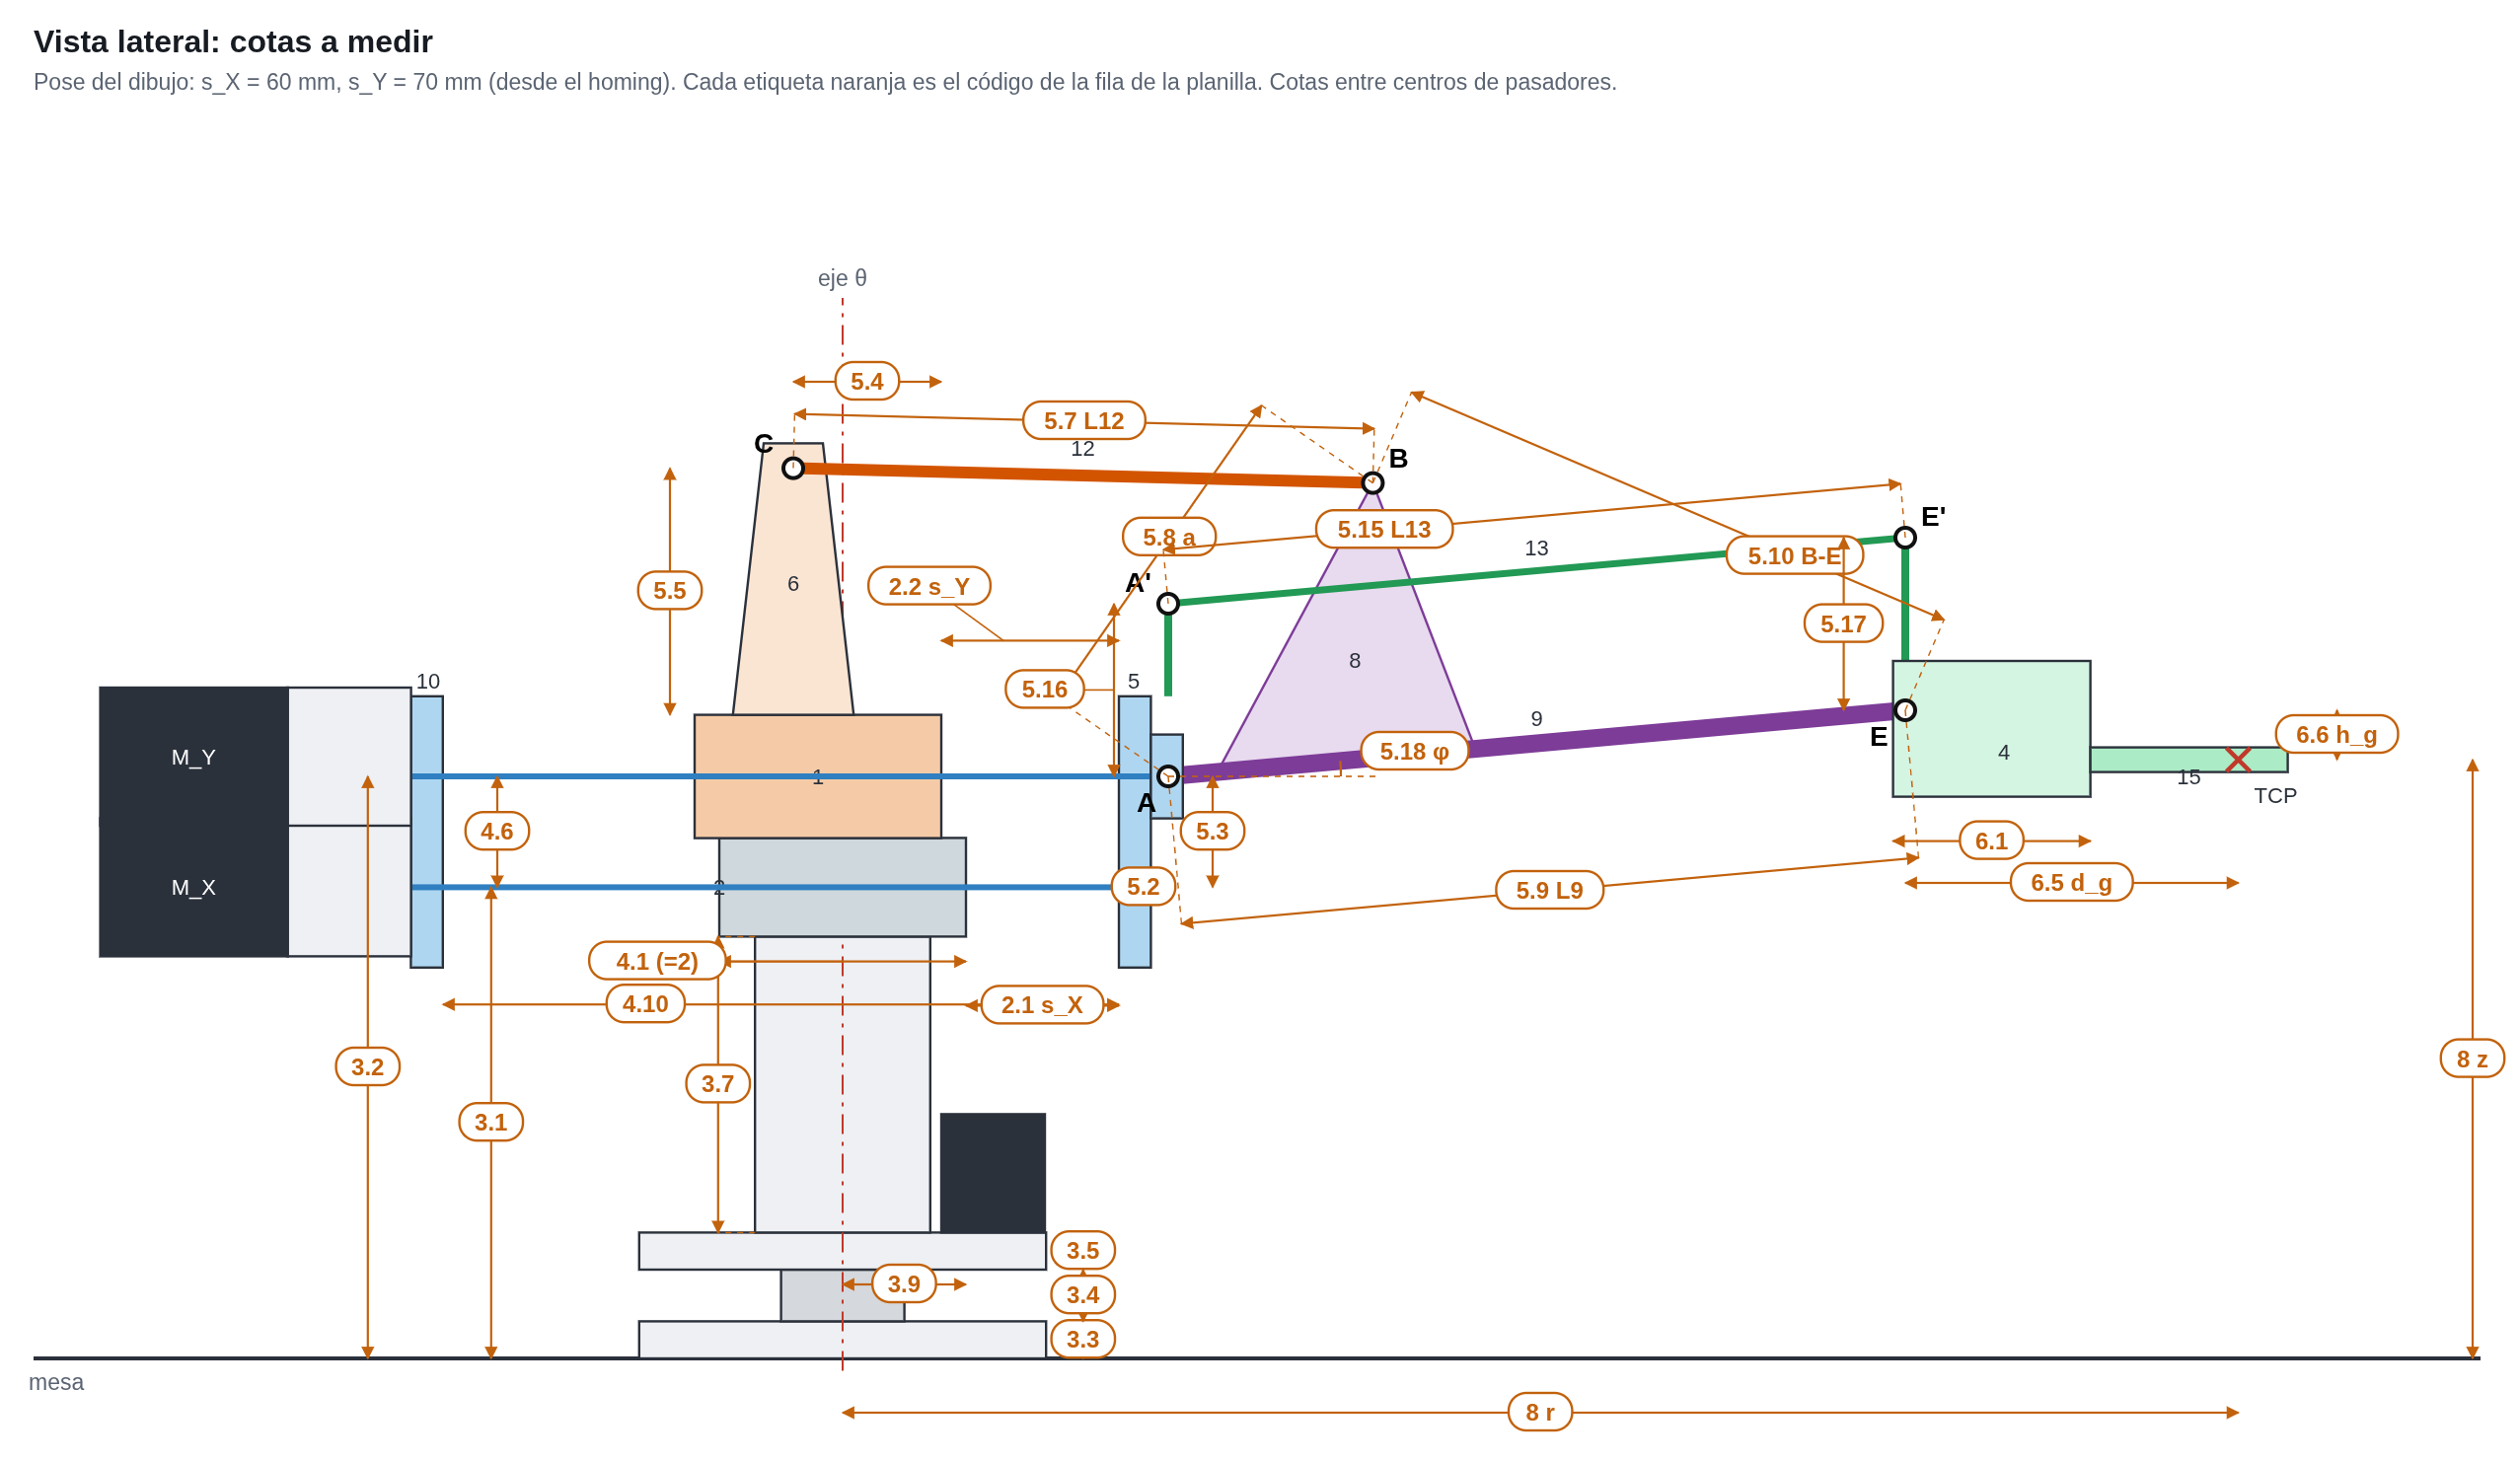
\includegraphics[width=\linewidth]{esquema_medidas_lateral.png}
\caption{Esquema de medidas en vista lateral (\texttt{levantamiento/esquema\_medidas\_lateral.png}).}
\end{figure}

\begin{center}\small
\begin{longtable}{>{\ttfamily}p{2.6cm} r >{\raggedright}p{2cm} >{\raggedright\arraybackslash}p{8cm}}
\toprule
\textbf{\rmfamily Parámetro} & \textbf{Valor} & \textbf{Origen} & \textbf{Significado}\\
\midrule
\endhead
largoGuias & 300 mm & leída & guías del bastidor\\
espesorPlaca & 13 mm & leída & placas extremas del bastidor\\
largoBloque & 100 mm & leída & bloques 1 y 2\\
holgura & 2 mm & SUPUESTO & distancia bloque--placa en el final de carrera\\
recorridoX, recorridoY & 170 mm & dato del equipo & $300 - 2\cdot13 - 100 - 2\cdot2$\\
sepNiveles & 45 mm & leída & separación entre los dos husillos\\
a & 145 mm & estimada & balancín A--B\\
beta ($\beta$) & 50° & estimada & ángulo entre A--B y el brazo\\
L12 & 235 mm & estimada & biela B--C\\
L9 & 300 mm & estimada & brazo A--E (igual a la varilla 13: paralelogramo)\\
dg, hg & 135, 20 mm & estimada & del pivote E al centro de las mordazas (TCP)\\
uA, dhA & 20, 45 mm & estimada & posición del pivote A en el bastidor\\
hC, dhC, uCBloque & 110, $-10$, $-60$ mm & leída / SUPUESTO / estimada & posición del pivote C en el bloque del carro Y\\
thetaMin, thetaMax & $\pm175$° & SUPUESTO & límite de giro por los cables\\
pasoHusillo & 5 mm & SUPUESTO & husillo SFU1605\\
micropasosXY & 5 (1000 p/vuelta) & leída & DIP de los drivers\\
\bottomrule
\end{longtable}
\end{center}
Todos los parámetros viven en un solo archivo, \codigo{web/js/cinematica.js}; el script \codigo{pruebas\_cinematica.js} los exporta a \codigo{modelo-3d/cinematica/parametros.json} para MATLAB y Python. De ellos se derivan, entre otros: altura del pivote A $h_A = 236$~mm, posición de la placa delantera con $s_X = 0$, $u_0 = 52$~mm, y la posición del pivote C respecto de A, $(c_{u0}, c_h) = (-252, 125)$~mm.

\section{El mecanismo}
\begin{figure}[H]
\centering
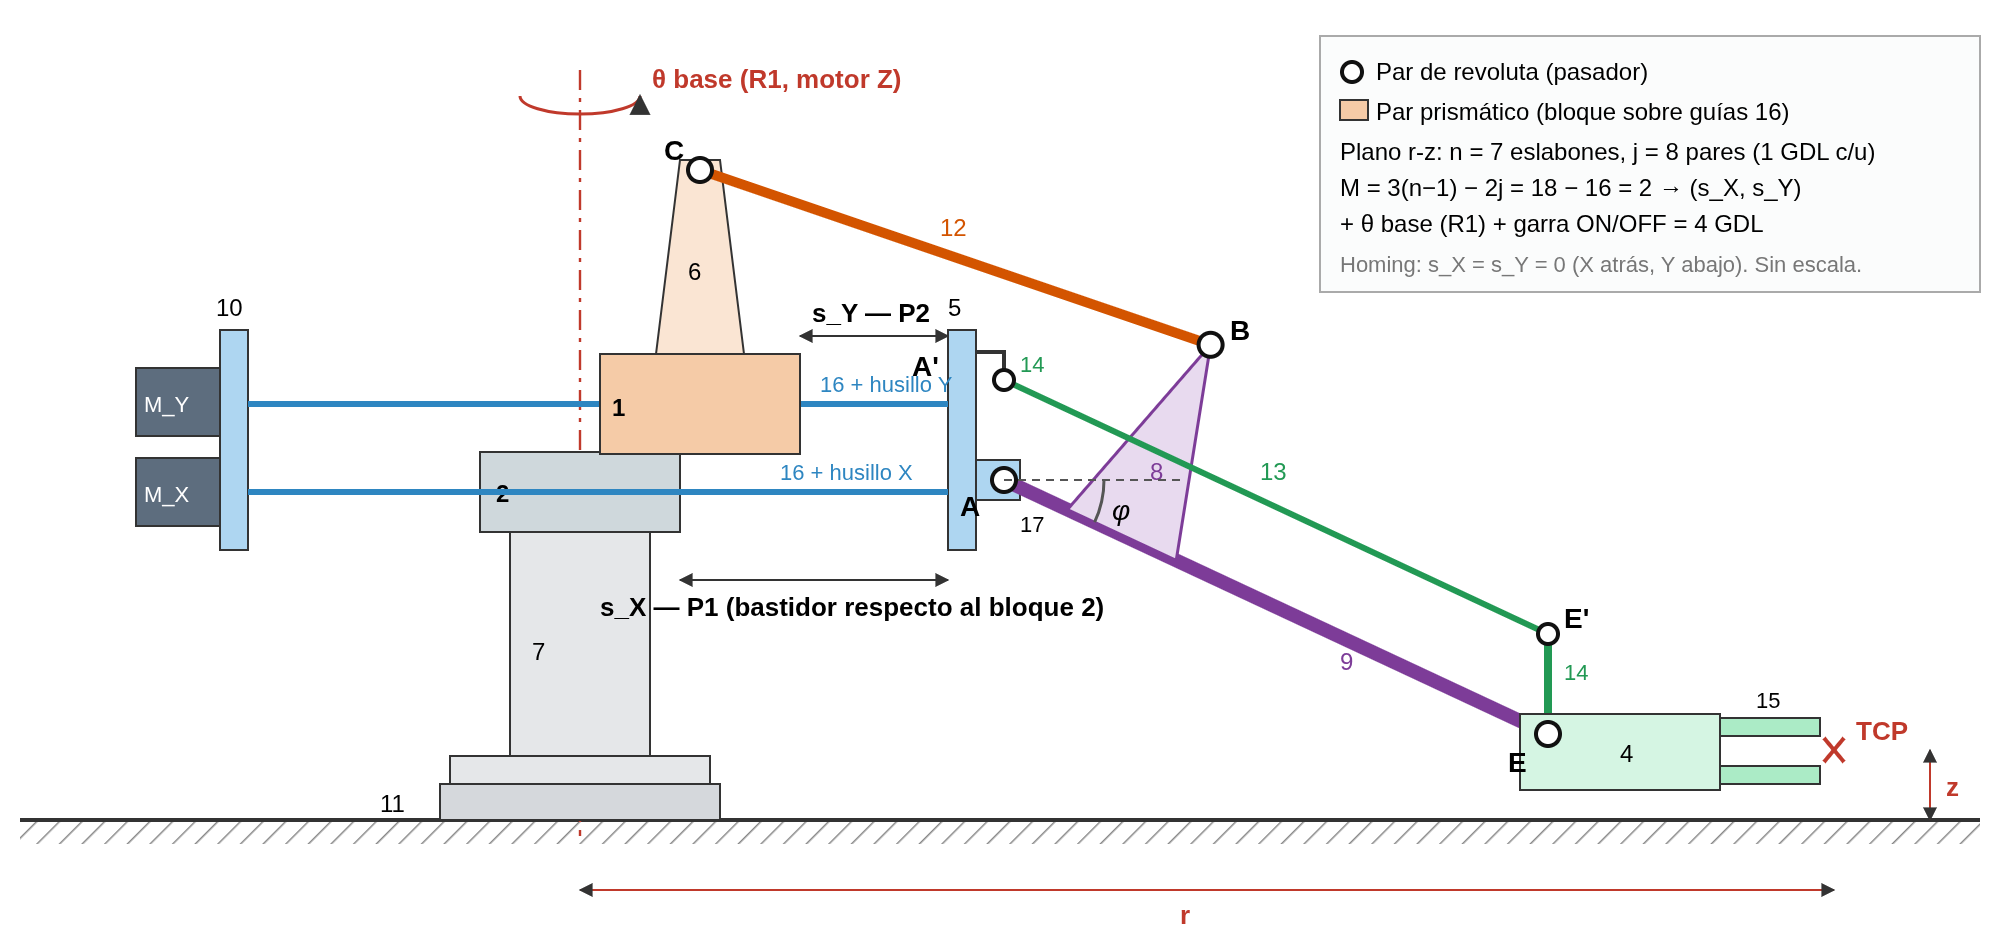
\includegraphics[width=\linewidth]{esquema_cinematico.png}
\caption{Esquema cinemático del brazo (\texttt{modelo-3d/informe/figuras/}).}
\end{figure}

El brazo trabaja en un plano vertical $(r, z)$ que gira con la base:
\begin{itemize}
\item el \textbf{carro X} desplaza todo el bastidor, y con él el pivote A del brazo: cambia el alcance;
\item el \textbf{carro Y} mueve el bloque 1 sobre el bastidor; la biela $L_{12}$ une el pivote C del bloque con el pivote B del balancín A--B, solidario al brazo: al moverse el bloque, el brazo gira un ángulo $\varphi$;
\item la varilla 13 forma un paralelogramo que mantiene la garra horizontal.
\end{itemize}

\begin{figure}[H]
\centering
\begin{tikzpicture}[x=1.05cm,y=1.05cm]
\coordinate (A) at (0,0); \coordinate (B) at (1.6,-1.0); \coordinate (C) at (4.3,-0.2);
\coordinate (E) at (6.2,2.3); \coordinate (T) at (7.6,2.0);
\draw[fill=gris] (-2.4,-2.6) rectangle (3.6,-1.9); \node[font=\scriptsize] at (0.6,-2.25) {carro X: desplaza todo el bastidor};
\draw[fill=naranja!20] (3.0,-1.0) rectangle (5.3,0.3); \node[font=\scriptsize] at (4.15,-1.4) {bloque del carro Y};
\draw[ultra thick, grisos] (A) -- (B) node[midway, left, font=\scriptsize]{$a$};
\draw[ultra thick, naranja] (B) -- (C) node[midway, below, font=\scriptsize]{$L_{12}$};
\draw[ultra thick, black] (A) -- (E) node[midway, above left, font=\scriptsize]{brazo $L_9$};
\draw[ultra thick, black] (E) -- (T);
\fill[naranja] (T) circle (0.12); \node[font=\scriptsize, right] at (T) {garra (TCP)};
\foreach \p in {A,B,C,E} {\fill[white] (\p) circle (0.11); \draw (\p) circle (0.11); \node[font=\scriptsize, above] at ($(\p)+(0,0.12)$) {\p};}
\draw[->] (A) ++(1.2,0) arc (0:35:1.2); \node[font=\scriptsize] at (1.6,0.45) {$\varphi$};
\draw[->] (A) ++(0.7,0) arc (0:-32:0.7); \node[font=\scriptsize] at (0.95,-0.25) {$\psi$};
\draw[<->] (3.0,0.7) -- (5.3,0.7) node[midway, above, font=\scriptsize]{$s_Y$};
\draw[<->] (-2.4,-2.9) -- (3.6,-2.9) node[midway, below, font=\scriptsize]{$s_X$};
\end{tikzpicture}
\caption{Esquema simplificado: lazo A--B--C y brazo A--E.}
\end{figure}

\section{Cinemática directa: de los carros a la garra}
Entrada $q = (\theta, s_X, s_Y)$; salida $(X, Y, Z)$ de la garra.

\paragraph{Paso 1: lazo de bielas.} La posición geométrica del bloque desde su tope trasero es $g = 170 - s_Y$ (el homing de Y deja el bloque adelante). El pivote C queda, respecto de A, en $C = (g + c_{u0},\, c_h) = (g - 252,\; 125)$. El pivote B está a distancia $a$ de A y a distancia $L_{12}$ de C: es la intersección de dos circunferencias. Con $d = |C|$,
\[
\psi = \operatorname{atan2}(c_h,\, g + c_{u0}) - \arccos\!\left(\frac{a^2 + d^2 - L_{12}^2}{2\,a\,d}\right),
\]
eligiendo el signo del montaje real (B por debajo de la recta A--C). El ángulo del brazo es $\varphi = \psi - \beta$.

\paragraph{Paso 2: posición de la garra en el plano.}
\[
r = u_0 + s_X + u_A + L_9\cos\varphi + d_g = 207 + s_X + 300\cos\varphi \quad [\text{mm}]
\]
\[
z = h_A + L_9\sin\varphi - h_g = 216 + 300\sin\varphi \quad [\text{mm}]
\]

\paragraph{Paso 3: giro de la base.} $X = r\cos\theta$, \ $Y = r\sin\theta$, \ $Z = z$.

\paragraph{Ejemplo resuelto: el homing $q = (0, 0, 0)$.} $g = 170$; $C = (-82, 125)$, $d = 149{,}5$~mm; $\arccos\frac{145^2 + 149{,}5^2 - 235^2}{2\cdot145\cdot149{,}5} = \arccos(-0{,}273) = 105{,}9°$; $\operatorname{atan2}(125, -82) = 123{,}3°$; $\psi = 17{,}4°$, $\varphi = -32{,}6°$. Luego $r = 207 + 0 + 300\cos(-32{,}6°) = 459{,}7$~mm y $z = 216 + 300\sin(-32{,}6°) = 54{,}4$~mm: la garra queda baja y cerca de la columna.

\begin{figure}[H]
\centering
\begin{minipage}[t]{0.49\linewidth}\centering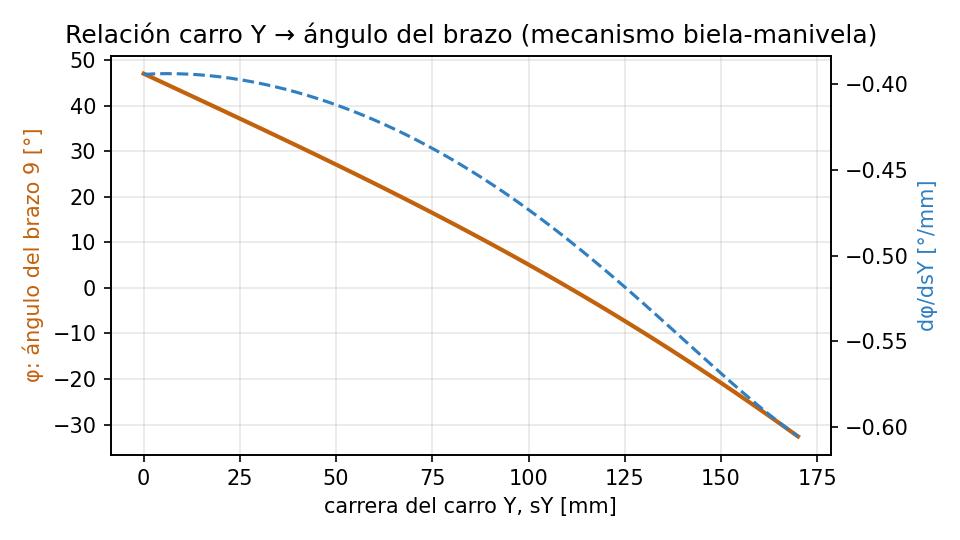
\includegraphics[width=\linewidth]{phi_vs_carro_y.png}\\{\small (a) ángulo del brazo $\varphi$ y su derivada frente a $s_Y$}\end{minipage}\hfill
\begin{minipage}[t]{0.49\linewidth}\centering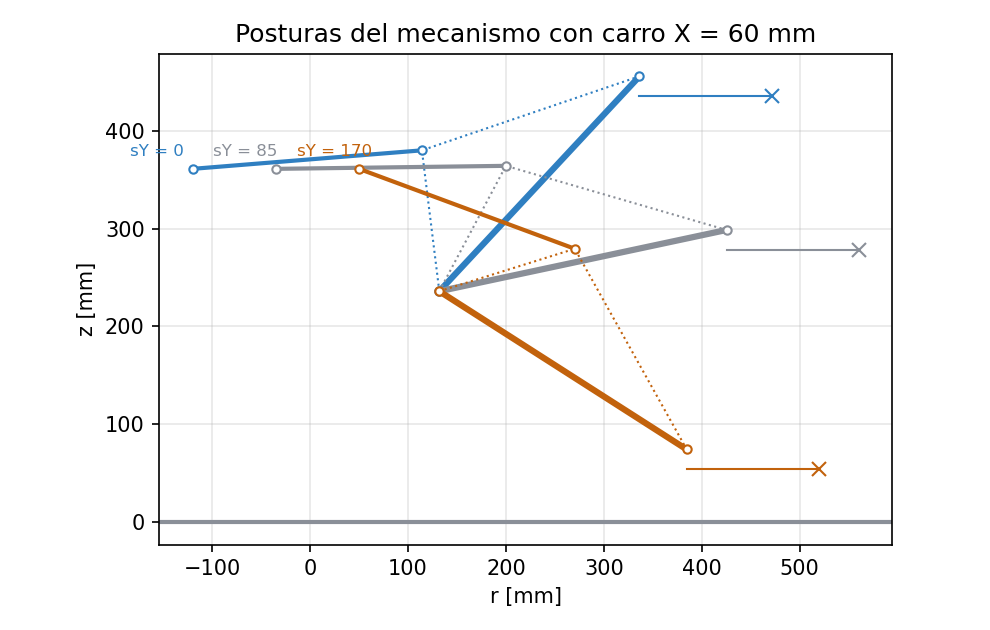
\includegraphics[width=\linewidth]{posturas_mecanismo.png}\\{\small (b) posturas del mecanismo con $s_X = 60$~mm}\end{minipage}
\caption{Relación entre el carro Y y el ángulo del brazo: de $-32{,}6°$ ($s_Y = 0$) a $+47{,}0°$ ($s_Y = 170$~mm), no lineal.}
\end{figure}

\section{Cinemática inversa: de la garra a los carros}
Entrada $(X, Y, Z)$; salida $q$.
\begin{enumerate}
\item $\theta = \operatorname{atan2}(Y, X)$, \ $r = \sqrt{X^2 + Y^2}$. Si hay varias soluciones ($\theta$ y $\theta \pm 360°$), se elige la más cercana a la actual.
\item De la altura: $\sin\varphi = \dfrac{Z + h_g - h_A}{L_9}$. Si $|\sin\varphi| > 1$, la altura es inalcanzable.
\item Del alcance: $s_X = r - d_g - L_9\cos\varphi - u_0 - u_A$.
\item Del lazo: con $\psi = \varphi + \beta$, $B = a(\cos\psi, \sin\psi)$; la biela exige $|B - C| = L_{12}$ con $C = (g - 252, 125)$:
\[
g = B_x + 252 \pm \sqrt{L_{12}^2 - (125 - B_z)^2}, \qquad s_Y = 170 - g,
\]
eligiendo la solución del montaje real.
\item Se descartan soluciones fuera de $0 \le s_X, s_Y \le 170$ o con la pinza chocando con la mesa.
\end{enumerate}

\paragraph{Ejemplo resuelto: garra en $(500, 200, 250)$~mm.} $\theta = \operatorname{atan2}(200, 500) = 21{,}80°$; $r = 538{,}52$~mm; $\sin\varphi = (250 + 20 - 236)/300 = 0{,}1133 \Rightarrow \varphi = 6{,}51°$; $s_X = 538{,}52 - 135 - 300\cos 6{,}51° - 52 - 20 = 33{,}45$~mm; $\psi = 56{,}51°$, $B = (80{,}0;\ 120{,}9)$; $g = 80{,}0 + 252 - \sqrt{235^2 - 4{,}1^2} = 97{,}05$~mm; $s_Y = 72{,}95$~mm. Comprobación con la directa: vuelve exactamente a $(500{,}000;\ 200{,}000;\ 250{,}000)$.

\section{Jacobiano y linealización}\label{sec:jacobiano}
El jacobiano relaciona pequeños movimientos de los ejes con pequeños movimientos de la garra:
\[
\Delta\mathbf{p} \approx J(q)\,\Delta q, \qquad
J = \frac{\partial(X, Y, Z)}{\partial(\theta, s_X, s_Y)} =
\begin{bmatrix}
-r\sin\theta & \cos\theta & \cos\theta\,\dfrac{\partial r}{\partial s_Y}\\[6pt]
r\cos\theta & \sin\theta & \sin\theta\,\dfrac{\partial r}{\partial s_Y}\\[6pt]
0 & 0 & \dfrac{\partial z}{\partial s_Y}
\end{bmatrix},
\]
con $\dfrac{\partial r}{\partial s_Y} = -L_9\sin\varphi\,\dfrac{d\varphi}{ds_Y}$ y $\dfrac{\partial z}{\partial s_Y} = L_9\cos\varphi\,\dfrac{d\varphi}{ds_Y}$. La derivada $d\varphi/ds_Y$ sale de derivar la ecuación del lazo $|a\,e(\psi) - C(g)|^2 = L_{12}^2$. Esta es la \textbf{linealización} del brazo alrededor de un punto de operación que pide la guía de laboratorio para la Fase 2: cerca de $q_0$, el brazo se comporta como el sistema lineal $\Delta\mathbf{p} = J(q_0)\Delta q$.

\begin{center}\small
\begin{longtable}{>{\raggedright}p{3cm} >{\centering}p{6.3cm} r r r}
\toprule
\textbf{Punto $q$} & \textbf{$J$ ($\theta$ en rad, mm/mm)} & \textbf{$\det J$} & \textbf{$d\varphi/ds_Y$} & \textbf{$\mu$}\\
\midrule
\endhead
$(0°, 0, 0)$ homing & $\begin{bmatrix}0 & 1 & 1{,}708\\ 459{,}7 & 0 & 0\\ 0 & 0 & 2{,}671\end{bmatrix}$ & 1228 & 0,606~°/mm & 37,7°\\[14pt]
$(0°, 85, 85)$ centro & $\begin{bmatrix}0 & 1 & -0{,}492\\ 585{,}4 & 0 & 0\\ 0 & 0 & 2{,}307\end{bmatrix}$ & 1350 & 0,451~°/mm & 61,3°\\[14pt]
$(30°, 120, 40)$ & $\begin{bmatrix}-311{,}3 & 0{,}866 & 0{,}411\\ 539{,}1 & 0{,}500 & 0{,}237\\ 0 & 0 & 2{,}725\end{bmatrix}$ & 1696 & 0,528~°/mm & 47,8°\\[14pt]
$(0°, 170, 170)$ esquina & $\begin{bmatrix}0 & 1 & -1{,}510\\ 581{,}5 & 0 & 0\\ 0 & 0 & 1{,}407\end{bmatrix}$ & 818 & 0,394~°/mm & 92,4°\\
\bottomrule
\end{longtable}
\end{center}

\paragraph{Cómo se lee.} En el centro $(0°, 85, 85)$: un milímetro del carro Y sube la garra 2,31~mm y la acerca 0,49~mm; un milímetro del carro X la aleja exactamente 1~mm; un grado de base la desplaza $585{,}4 \cdot \pi/180 = 10{,}2$~mm de lado. Es decir, el carro Y \emph{amplifica} su movimiento en altura por más de 2.

\paragraph{Qué tan buena es la linealización.} Comparación con la cinemática exacta desde el centro:
\begin{center}\small
\begin{tabular}{@{}lccc@{}}
\toprule
$\Delta q = (\Delta\theta, \Delta s_X, \Delta s_Y)$ & exacto $\Delta(X, Y, Z)$ [mm] & lineal $J\Delta q$ [mm] & error\\
\midrule
$(0°, 2, 2)$ & (0,98; 0; 4,59) & (1,02; 0; 4,61) & 0,04~mm\\
$(2°, 0, 0)$ & ($-0{,}36$; 20,43; 0) & (0; 20,43; 0) & 0,36~mm\\
$(0°, 10, 10)$ & (4,28; 0; 22,52) & (5,08; 0; 23,07) & 0,97~mm\\
$(5°, 0, -10)$ & (1,82; 51,38; $-23{,}61$) & (4,92; 51,09; $-23{,}07$) & 3,2~mm\\
\bottomrule
\end{tabular}
\end{center}
La aproximación es excelente para movimientos de pocos milímetros y empeora con desplazamientos grandes, sobre todo de la base (el arco no es una recta). Por eso la página recalcula la inversa en cada punto de una trayectoria en lugar de usar solo el jacobiano.

\paragraph{Singularidades y transmisión.} Como $\det J = r\,\partial z/\partial s_Y$ y en todo el recorrido $r > 400$~mm y $\partial z/\partial s_Y > 1{,}4$, el determinante nunca se anula: \textbf{no hay singularidades dentro del recorrido}. El \emph{ángulo de transmisión} $\mu$ entre la biela y el balancín (ideal 90°) mide qué tan bien la biela empuja al brazo: vale 37,7° en el homing (transmisión pobre, el carro Y necesita más fuerza) y 92,4° con el brazo arriba.

\section{Espacio de trabajo}
\begin{figure}[H]
\centering
\begin{minipage}[t]{0.56\linewidth}\centering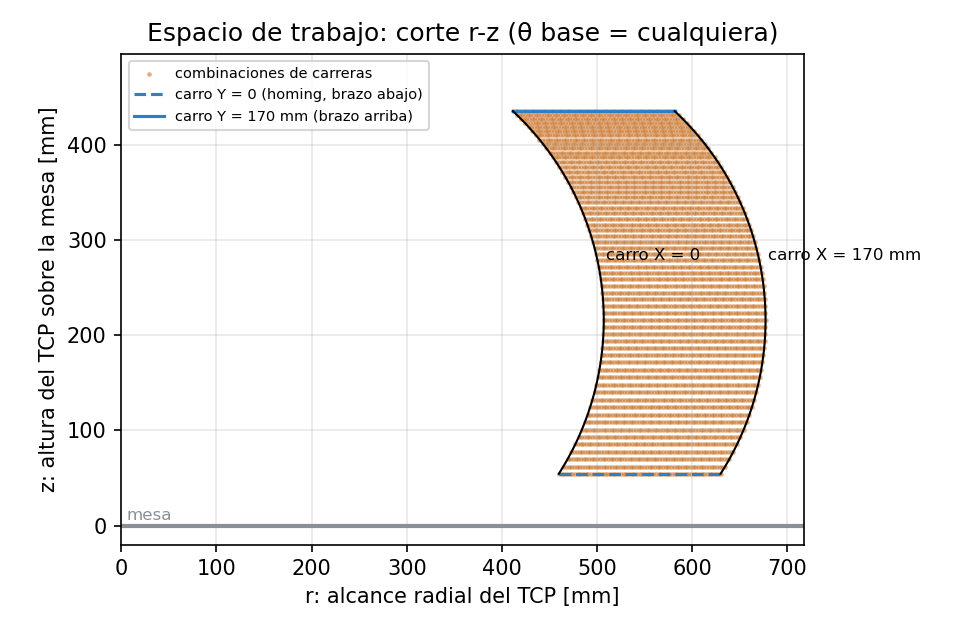
\includegraphics[width=\linewidth]{espacio_trabajo_rz.png}\\{\small (a) corte vertical $(r, z)$}\end{minipage}\hfill
\begin{minipage}[t]{0.42\linewidth}\centering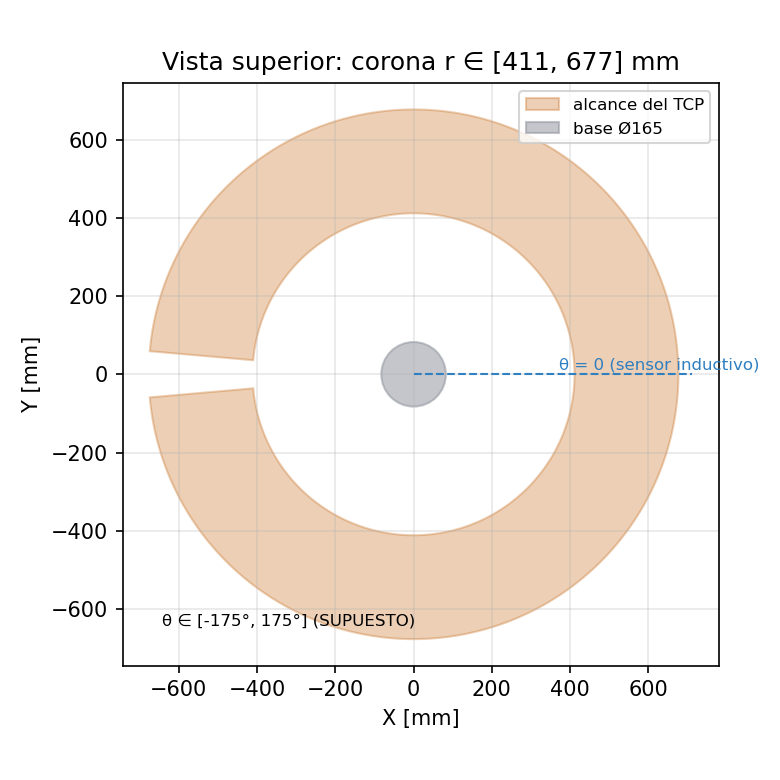
\includegraphics[width=\linewidth]{espacio_trabajo_superior.png}\\{\small (b) vista superior}\end{minipage}
\caption{Espacio de trabajo: una franja curva en el plano vertical que gira con la base; alcance radial de 411 a 677~mm.}
\end{figure}
Desde el homing (esquina inferior izquierda de la franja), un movimiento vertical de la garra sale de la zona alcanzable: por eso muchos puntos escritos a mano resultan inalcanzables, y la app propone el punto alcanzable más cercano.

\section{Modelo 3D}
Las piezas se modelaron con las mismas cotas y se ensamblaron en \codigo{global/modelo-3d/brazo\_xk-js1-1.glb}, generado por el script \codigo{generar\_modelo.js} (sin programas de diseño). El visor (three.js) coloca cada pieza según la cinemática directa en cada cuadro.

\begin{figure}[H]
\centering
\begin{minipage}[t]{0.49\linewidth}\centering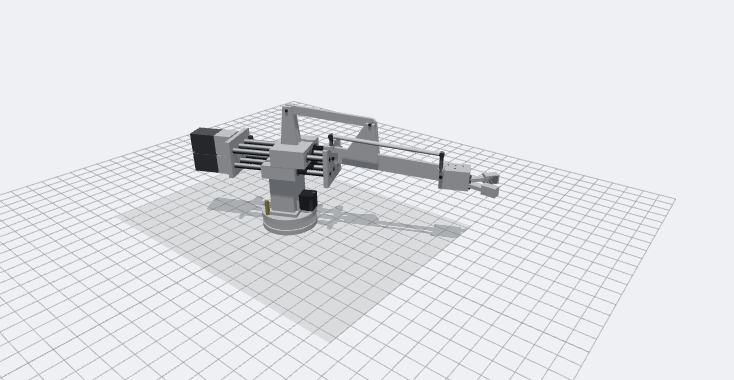
\includegraphics[width=\linewidth]{modelo_3d_isometrica.png}\\{\small (a) isométrica}\end{minipage}\hfill
\begin{minipage}[t]{0.49\linewidth}\centering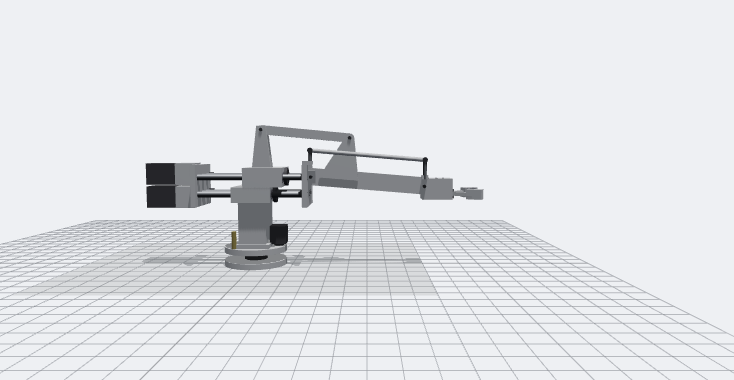
\includegraphics[width=\linewidth]{modelo_3d_lateral.png}\\{\small (b) lateral}\end{minipage}
\caption{Modelo 3D del brazo.}
\end{figure}

\section{Scripts del modelado}
\begin{center}\small
\begin{tabularx}{\linewidth}{>{\raggedright}p{6.2cm} >{\raggedright\arraybackslash}X}
\toprule
\textbf{Archivo} & \textbf{Qué hace}\\
\midrule
\codigo{web/js/cinematica.js} & modelo: parámetros, directa, inversa, jacobiano, espacio de trabajo, pulsos, trayectorias\\
\codigo{modelo-3d/cinematica/pruebas\_cinematica.js} & pruebas: la inversa de la directa devuelve el mismo $q$; exporta \codigo{parametros.json} y \codigo{tabla\_cinematica.csv}\\
\codigo{modelo-3d/cinematica/cinematica\_brazo.m} & la misma cinemática en MATLAB\\
\codigo{modelo-3d/cinematica/graficas\_cinematica.py} & gráficas del informe (espacio de trabajo, $\varphi(s_Y)$, posturas)\\
\codigo{modelo-3d/levantamiento/generar\_esquema\_medidas.py} & esquemas acotados del levantamiento\\
\codigo{global/modelo-3d/generar\_modelo.js} & genera el modelo 3D \codigo{.glb}\\
\bottomrule
\end{tabularx}
\end{center}

\begin{lstlisting}[style=js, caption={Cinemática inversa (fragmento de \texttt{web/js/cinematica.js}).}]
const s = (obj.Z + p.hg - d.hA) / p.L9;           // seno del ángulo del brazo
if (Math.abs(s) > 1) return { valida: false, motivo: 'Altura inalcanzable' };
for (const [rama, phi] of [['adelante', Math.asin(s)], ['atrás', Math.PI - Math.asin(s)]]) {
  const sX = r - p.dg - p.L9 * Math.cos(phi) - d.u5_0 - p.uA;   // alcance -> carro X
  const psi = phi + beta;                                         // balancín A-B
  const bx = p.a * Math.cos(psi), bz = p.a * Math.sin(psi);
  const disc = p.L12 * p.L12 - (d.ch - bz) * (d.ch - bz);         // biela L12 hasta C
  if (disc < 0) continue;
  // dos posiciones posibles del bloque; se queda la del montaje real
}
\end{lstlisting}

% =====================================================================
\chapter{Protocolo de comunicación PLC--PC: PPI}\label{cap:ppi}

\section{Qué es PPI y por qué se usó}
PPI (\emph{Point-to-Point Interface}) es el protocolo con el que STEP 7-Micro/WIN programa y monitorea los S7-200. Es un protocolo \textbf{maestro--esclavo} sobre RS-485, derivado de PROFIBUS-FDL: la PC es el maestro (dirección 0) y el PLC el esclavo (hoy, dirección 2). Dentro de las tramas PPI viajan mensajes \textbf{S7} que leen o escriben zonas de memoria.

\begin{center}\small
\begin{tabularx}{\linewidth}{>{\raggedright}p{3.4cm} >{\raggedright}X >{\raggedright\arraybackslash}X}
\toprule
& \textbf{PPI} (elegido) & \textbf{Modbus RTU} (guía, Fase 3)\\
\midrule
Hardware & el cable USB-PPI que ya tenía el laboratorio & el mismo puerto RS-485\\
Programa del PLC & no hay que programar la comunicación: el sistema operativo del PLC responde solo & hay que programarla en modo \emph{Freeport} o con la librería Modbus de Micro/WIN, y el puerto deja de servir para programar mientras está activa\\
Acceso & cualquier zona de memoria (I, Q, M, V, SM) & solo los registros que el programa mapea\\
Herramientas & poco documentado: se programó desde cero en Python & muy documentado, muchas herramientas\\
\bottomrule
\end{tabularx}
\end{center}
PPI permitió leer el programa original \emph{sin modificarlo} (las primeras pruebas fueron de solo lectura) y seguir usando Micro/WIN con el mismo cable. El cliente está en \codigo{app/ppi.py} y \codigo{app/serie.py}, sin bibliotecas externas.

\begin{figure}[H]
\centering
\begin{tikzpicture}
\node[draw, fill=gris, minimum width=12cm, minimum height=26mm] (c1) {};
\node[anchor=north west, font=\scriptsize\bfseries] at (c1.north west) {Capa física: RS-485 (par diferencial, semidúplex), 8 bits + paridad par + 1 parada};
\node[draw, fill=white, minimum width=10.6cm, minimum height=17mm] (c2) at ($(c1.center)+(0,-2mm)$) {};
\node[anchor=north west, font=\scriptsize\bfseries] at (c2.north west) {Enlace PPI: tramas SD1/SD2/SC, direcciones, control FC, suma FCS};
\node[draw, fill=naranja!14, minimum width=9cm, minimum height=8mm] (c3) at ($(c2.center)+(0,-2.5mm)$) {\scriptsize \textbf{Aplicación S7}: «leer 40 bytes desde VB1120», «escribir VB1100--VB1119»};
\end{tikzpicture}
\caption{Capas del protocolo.}
\end{figure}

\section{Capa física}
\begin{figure}[H]
\centering
\begin{tikzpicture}[x=1cm,y=1cm]
\draw[thick, rounded corners=6pt, fill=gris] (0,0) -- (4.2,0) -- (3.8,-1.6) -- (0.4,-1.6) -- cycle;
\foreach \i in {1,...,5} { \pgfmathsetmacro\xx{0.5+0.8*(\i-1)} \fill (\xx,-0.45) circle (0.13); \node[font=\tiny, above] at (\xx,-0.3) {\i}; }
\foreach \i in {6,...,9} { \pgfmathsetmacro\xx{0.9+0.8*(\i-6)} \fill (\xx,-1.15) circle (0.13); \node[font=\tiny, below] at (\xx,-1.3) {\i}; }
\node[font=\scriptsize\bfseries] at (2.1,0.45) {puerto 0 del PLC (DB9 hembra)};
\node[etiq, align=left, anchor=west] at (4.6,-0.15) {pin 3: B (+), datos};
\node[etiq, align=left, anchor=west] at (4.6,-0.55) {pin 8: A ($-$), datos};
\node[etiq, align=left, anchor=west] at (4.6,-0.95) {pin 5: tierra (GND)};
\node[etiq, align=left, anchor=west] at (4.6,-1.35) {pin 2: 24 V (alimenta el cable)};
\node[caja, text width=2.8cm, font=\scriptsize] (conv) at (9.8,-0.6) {cable USB-PPI\\CH340 (USB$\leftrightarrow$serie)\\+ transceptor RS-485\\cambio de sentido automático};
\node[cajab, font=\scriptsize] (pcn) at (12.9,-0.6) {PC\\\codigo{/dev/ttyUSB0}\\o \codigo{COM3}};
\draw[dflecha] (7.0,-0.6) -- (conv.west); \draw[dflecha] (conv) -- node[above, etiq]{USB} (pcn);
\begin{scope}[shift={(0,-3.4)}]
\draw[->] (0,0) -- (8.8,0) node[right, etiq]{t};
\node[etiq, left] at (0,0.7) {B}; \node[etiq, left] at (0,-0.7) {A};
\draw[thick, naranja] (0,0.8) -- (1,0.8) -- (1,0.3) -- (2.6,0.3) -- (2.6,0.8) -- (4.2,0.8) -- (4.2,0.3) -- (5,0.3) -- (5,0.8) -- (8.5,0.8);
\draw[thick, azulg] (0,-0.8) -- (1,-0.8) -- (1,-0.3) -- (2.6,-0.3) -- (2.6,-0.8) -- (4.2,-0.8) -- (4.2,-0.3) -- (5,-0.3) -- (5,-0.8) -- (8.5,-0.8);
\node[etiq, text width=4.6cm, align=left, anchor=west] at (9.1,0) {el receptor mira $V_B - V_A$: positivo = 1, negativo = 0; el ruido común a los dos hilos se cancela};
\end{scope}
\end{tikzpicture}
\caption{Conector, cable y señal diferencial RS-485 (esquemática).}
\end{figure}

\begin{figure}[H]
\centering
\begin{tikzpicture}[x=1.05cm,y=1cm]
\foreach \i/\t/\c in {0/inicio/gris, 1/b0/white, 2/b1/white, 3/b2/white, 4/b3/white, 5/b4/white, 6/b5/white, 7/b6/white, 8/b7/white, 9/paridad/naranja!20, 10/parada/gris} {
  \draw[fill=\c] (\i,0) rectangle ++(1,0.8); \node[font=\scriptsize] at (\i+0.5,0.4) {\t};}
\draw[decorate, decoration={brace, amplitude=5pt}] (1,0.9) -- (9,0.9) node[midway, above=5pt, etiq]{8 bits de datos, el menos significativo primero};
\draw[decorate, decoration={brace, amplitude=5pt, mirror}] (0,-0.1) -- (11,-0.1) node[midway, below=5pt, etiq]{11 bits: a 9600 bit/s un byte tarda 1,146 ms; a 19\,200 bit/s, 0,573 ms};
\end{tikzpicture}
\caption{Formato de cada carácter: 8 bits, paridad par, 1 bit de parada (8E1).}
\end{figure}

\section{Tramas}
\begin{figure}[H]
\centering
\begin{tikzpicture}[x=1cm,y=1cm, byte/.style={draw, minimum width=8.5mm, minimum height=7mm, font=\ttfamily\scriptsize, inner sep=0pt, anchor=west}]
\node[anchor=west, font=\small\bfseries] at (0,0.75) {SD2: longitud variable (con datos)};
\foreach \i/\t/\c in {0/68/naranja!20, 1/LE/white, 2/LEr/white, 3/68/naranja!20, 4/DA/azulg!15, 5/SA/azulg!15, 6/FC/azulg!15} {\node[byte, fill=\c] at (\i*0.95,0) {\t};}
\node[byte, fill=white, minimum width=36mm] at (6.65,0) {datos (mensaje S7)};
\node[byte, fill=verde!15] at (10.5,0) {FCS}; \node[byte, fill=naranja!20] at (11.45,0) {16};
\node[anchor=west, font=\small\bfseries] at (0,-0.95) {SD1: corta, sin datos (sondeo)};
\foreach \i/\t/\c in {0/10/naranja!20, 1/DA/azulg!15, 2/SA/azulg!15, 3/FC/azulg!15, 4/FCS/verde!15, 5/16/naranja!20} {\node[byte, fill=\c] at (\i*0.95,-1.7) {\t};}
\node[anchor=west, font=\small\bfseries] at (0,-2.65) {SC: acuse de un byte};
\node[byte, fill=naranja!20] at (0,-3.4) {E5};
\end{tikzpicture}
\caption{Formatos de trama PPI.}
\end{figure}

\begin{center}\small
\begin{tabularx}{\linewidth}{>{\ttfamily}p{1.8cm} >{\raggedright\arraybackslash}X}
\toprule
\textbf{\rmfamily Campo} & \textbf{Significado}\\
\midrule
68 / 10 & delimitador de inicio de SD2 / SD1\\
LE, LEr & longitud de DA + SA + FC + datos, repetida\\
DA, SA & dirección de destino y de origen (PC = 0, PLC = 2)\\
FC & control: \codigo{6C}/\codigo{7C} petición (el bit FCB alterna para distinguir una trama nueva de una repetida); \codigo{5C}/\codigo{7C} sondeo; \codigo{08} respuesta con datos\\
FCS & suma de DA, SA, FC y los datos, módulo 256\\
16 & delimitador de fin\\
E5 & acuse: «recibí tu trama» o «todavía no tengo la respuesta»\\
\bottomrule
\end{tabularx}
\end{center}

\section{Intercambio y tiempos medidos}
\begin{figure}[H]
\centering
\begin{tikzpicture}[x=1cm,y=1cm]
\node[caja, minimum width=2.6cm] at (0,0) {PC (maestro, 0)};
\node[caja, minimum width=2.6cm] at (8,0) {PLC (esclavo, 2)};
\draw[black!40, dashed] (0,-0.5) -- (0,-6.3); \draw[black!40, dashed] (8,-0.5) -- (8,-6.3);
\draw[flecha] (0,-1.0) -- node[above, etiq]{1. SD2 petición S7 (33 bytes, $\approx$38 ms)} (8,-1.3);
\draw[flecha] (8,-1.9) -- node[above, etiq]{2. \codigo{E5} acuse} (0,-2.1);
\node[etiq, left, text width=2.6cm, align=right] at (-0.2,-2.6) {silencio $\geq$ 150 bits ($\approx$16 ms)};
\draw[flecha] (0,-3.1) -- node[above, etiq]{3. SD1 sondeo (6 bytes)} (8,-3.3);
\draw[flecha] (8,-3.9) -- node[above, etiq]{4. SD2 respuesta con datos (67 bytes, $\approx$77 ms)} (0,-4.6);
\node[etiq, right, text width=3.2cm] at (8.2,-1.6) {el PLC atiende entre ciclos de su programa};
\draw[decorate, decoration={brace, amplitude=5pt, mirror}] (-2.9,-0.9) -- (-2.9,-4.7) node[midway, left=6pt, etiq]{$\approx$155 ms\\en total};
\node[etiq, text width=12cm, align=left, anchor=west] at (-2.9,-5.6) {Si en el paso 3 el PLC aún no tiene la respuesta, contesta \codigo{E5} y la PC repite el sondeo (hasta 8 veces).};
\end{tikzpicture}
\caption{Lectura de 40 bytes a 9,6~kbit/s con los tiempos medidos en la planta.}
\end{figure}

\section{Mensajes S7: ejemplos byte a byte}
\subsection{Lectura del estado}
\begin{figure}[H]
\centering
\begin{tikzpicture}[x=0.93cm,y=1cm, byte/.style={draw, minimum width=8mm, minimum height=7mm, font=\ttfamily\scriptsize, inner sep=0pt, anchor=west}]
\def\fila#1#2{\foreach \t [count=\i from 0] in {#2} {\node[byte] at (\i*0.93,#1) {\t};}}
\fila{0}{68,1b,1b,68,02,00,6c}
\fila{-1.4}{32,01,00,00,00,01,00,0e,00,00}
\fila{-2.8}{04,01}
\fila{-4.2}{12,0a,10,02,00,28,00,01,84,00,23,00}
\fila{-5.6}{b3,16}
\node[etiq, anchor=west, text width=8cm, align=left] at (7.0,0) {\textbf{PPI}: inicio, longitud 27, PLC 2, PC 0, petición (\codigo{6c})};
\node[etiq, anchor=west, text width=6cm, align=left] at (9.6,-1.4) {\textbf{cabecera S7}: \codigo{32} protocolo, \codigo{01} petición, referencia 1, 14 bytes de parámetros, 0 de datos};
\node[etiq, anchor=west, text width=8cm, align=left] at (2.2,-2.8) {\textbf{función}: \codigo{04} leer, \codigo{01} una zona};
\node[etiq, anchor=west, text width=4.2cm, align=left] at (11.4,-4.2) {\textbf{zona}: bytes (\codigo{02}), 40 (\codigo{0028}), DB 1, área V (\codigo{84}), dirección en bits $1120 \times 8 = 8960$ = \codigo{002300}};
\node[etiq, anchor=west, text width=8cm, align=left] at (2.2,-5.6) {\textbf{FCS} = (\codigo{02}+\codigo{00}+\codigo{6c}+\dots+\codigo{00}) mod 256 = 435 mod 256 = \codigo{b3}; fin};
\end{tikzpicture}
\caption{Petición «leer 40 bytes desde VB1120».}
\end{figure}
La respuesta (67 bytes) trae: cabecera PPI con las direcciones invertidas y FC \codigo{08}; cabecera S7 de tipo \codigo{03} (respuesta) con código de error 0; función \codigo{04 01}; \codigo{FF} (lectura correcta), \codigo{04} (bytes), longitud en bits \codigo{0140} (320 bits) y los 40 bytes de estado.

\subsection{Escritura de una orden}
Orden «mover X +4000 pulsos (20~mm) e Y $-$2000 pulsos ($-$10~mm)», secuencia 5, latido 7, ciclos 250 y 400~µs. La app empaqueta los 20 bytes del buzón con \codigo{struct.pack('>BBHiiiHH', ...)} (big-endian, como el PLC):

\begin{center}\small
\begin{tabular}{@{}llll@{}}
\toprule
\textbf{Bytes} & \textbf{Campo} & \textbf{Hex} & \textbf{Valor}\\
\midrule
VB1100 & orden & \codigo{02} & mover\\
VB1101 & secuencia & \codigo{05} & 5\\
VW1102 & latido & \codigo{00 07} & 7\\
VD1104 & pulsos base & \codigo{00 00 00 00} & 0\\
VD1108 & pulsos X & \codigo{00 00 0f a0} & +4000\\
VD1112 & pulsos Y & \codigo{ff ff f8 30} & $-$2000 (complemento a 2)\\
VW1116 & ciclo X/Y & \codigo{00 fa} & 250~µs\\
VW1118 & ciclo base & \codigo{01 90} & 400~µs\\
\bottomrule
\end{tabular}
\end{center}
Trama completa (57 bytes):
\begin{lstlisting}
68 33 33 68 02 00 7c                        PPI: longitud 51, PLC 2, PC 0, petición
32 01 00 00 00 01 00 0e 00 18               S7: petición, 14 bytes de parámetros, 24 de datos
05 01 12 0a 10 02 00 14 00 01 84 00 22 60   escribir 1 zona: 20 bytes en V, bit 8800 (VB1100)
00 04 00 a0                                 datos: tipo bytes, 160 bits
02 05 00 07 00 00 00 00 00 00 0f a0 ff ff f8 30 00 fa 01 90
39 16                                       FCS = 2105 mod 256 = 0x39; fin
\end{lstlisting}
La app solo puede escribir en las zonas autorizadas para el programa reconocido (VB1100--VB1119 con \codigo{brazo\_gemelo}); cualquier otra dirección se rechaza en \codigo{ppi.py} antes de salir por el cable.

\section{Lo aprendido en la planta}
\begin{itemize}
\item \textbf{Silencio entre tramas.} A 9,6~kbit/s el PLC ignoraba la trama que llegaba pegada a la anterior: el primer sondeo se perdía y se esperaban 0,4~s. Con un silencio de unos 150 bits antes de transmitir, las lecturas bajaron de 568~ms a 155~ms y dejaron de fallar.
\item \textbf{Búsqueda automática.} Si cambia la dirección o la velocidad del PLC (al cargar un bloque de sistema), la app prueba primero 2, 6 y 7 a 9,6 y 19,2~kbit/s, y luego las 31 direcciones posibles.
\item \textbf{Un solo maestro.} El cable lo usa la app o Micro/WIN, nunca los dos a la vez.
\end{itemize}

\begin{figure}[H]
\centering
\begin{tikzpicture}[x=0.018cm,y=1cm]
\node[anchor=east, font=\scriptsize] at (-10,0.3) {antes};
\fill[naranja!60] (0,0) rectangle (43,0.6);
\fill[rojo!25] (44,0) rectangle (446,0.6); \node[font=\scriptsize] at (245,0.3) {sondeo ignorado: espera 0,4 s};
\fill[azulg!40] (456,0) rectangle (479,0.6); \fill[verde!45] (479,0) rectangle (568,0.6);
\node[anchor=west, font=\scriptsize] at (575,0.3) {568 ms};
\node[anchor=east, font=\scriptsize] at (-10,-0.6) {después};
\fill[naranja!60] (0,-0.9) rectangle (43,-0.3); \fill[gris] (43,-0.9) rectangle (60,-0.3);
\fill[azulg!40] (60,-0.9) rectangle (67,-0.3); \fill[verde!45] (67,-0.9) rectangle (155,-0.3);
\node[anchor=west, font=\scriptsize] at (162,-0.6) {155 ms};
\draw[->] (0,-1.15) -- (620,-1.15) node[right, font=\scriptsize]{ms};
\foreach \t in {0,100,...,600} {\draw (\t,-1.1) -- (\t,-1.2) node[below, font=\tiny]{\t};}
\end{tikzpicture}
\caption{Tiempo de una lectura antes y después del silencio entre tramas (naranja: petición; azul: sondeo; verde: respuesta).}
\end{figure}

\begin{lstlisting}[style=py, caption={Núcleo del intercambio (\texttt{app/ppi.py}).}]
def _intercambio(self, pdu):
    self.p.vaciar_entrada()
    self._pausa()                              # silencio de ~150 bits: el PLC lo necesita
    self.p.escribir(self._sd2(0x7C if self._fcb else 0x6C, pdu))
    self._fcb = not self._fcb
    if not self._leer(0.4).startswith(b'\xe5'):
        raise ErrorPPI('el PLC no acusó la petición')
    for intento in range(8):                   # sondeo hasta que llegue la respuesta
        self._pausa()
        self.p.escribir(self._sd1(0x5C if intento % 2 == 0 else 0x7C))
        r = self._leer(0.4)
        if r.startswith(b'\x68'):
            return r[7:4 + r[1]]               # mensaje S7 (tras verificar la suma)
\end{lstlisting}

\section{Limitaciones}
A 9,6~kbit/s caben unas 6 lecturas por segundo: suficiente para ver y mandar el brazo, no para un lazo de control rápido desde la PC. Por eso los movimientos los ejecuta el PLC y la PC solo envía destinos. Volver a 19,2~kbit/s en el bloque de sistema duplicaría la frecuencia de lectura.

% =====================================================================
\chapter{Las aplicaciones}\label{cap:aplicaciones}

\section{Panorama}
\begin{center}\small
\begin{tabularx}{\linewidth}{>{\raggedright}p{3.6cm} >{\raggedright}p{3.8cm} >{\raggedright\arraybackslash}X}
\toprule
\textbf{Aplicación} & \textbf{Dónde corre} & \textbf{Para qué}\\
\midrule
STEP 7-Micro/WIN & máquina virtual Windows XP (VirtualBox) en la PC de Linux; o Windows directo & editar, compilar y cargar los programas del PLC; el USB del cable se pasa a la VM desde \emph{Dispositivos $\rightarrow$ USB}\\
App del gemelo (\codigo{app/}) & PC del laboratorio, Linux o Windows, Python 3 & conectar con el PLC, ver y mandar el brazo; menú de tres modos; acceso por red\\
Página publicada & internet (GitHub Pages y Cloudflare Pages) & documentación del proyecto, simulación del brazo, catálogo de archivos\\
Scripts de modelado & cualquier PC (Node.js, Python, MATLAB) & cinemática, gráficas, modelo 3D\\
\bottomrule
\end{tabularx}
\end{center}

\section{Arquitectura de tres capas}
La guía 1 pide pensar el sistema en tres capas. Así quedaron:
\begin{figure}[H]
\centering
\begin{tikzpicture}[node distance=5mm and 10mm, capa/.style={draw, rounded corners=3pt, fill=gris!60, minimum width=4.2cm, minimum height=48mm, align=center, font=\small\bfseries, anchor=north}]
\node[capa] (c1) at (0,0) {};
\node[capa] (c2) at (5,0) {};
\node[capa] (c3) at (10,0) {};
\node[font=\small\bfseries, below=1mm of c1.north] {Campo y control};
\node[font=\small\bfseries, below=1mm of c2.north] {Aplicación (middleware)};
\node[font=\small\bfseries, below=1mm of c3.north] {Datos y presentación};
\node[cajab, text width=3.4cm, font=\scriptsize] at (0,-1.6) {sensores, panel, drivers, motores};
\node[cajan, text width=3.4cm, font=\scriptsize] at (0,-3.4) {PLC S7-200 con \codigo{brazo\_gemelo}: cuenta, protege, ejecuta};
\node[cajab, text width=3.4cm, font=\scriptsize] at (5,-1.6) {\codigo{ppi.py} + \codigo{serie.py}: lee y escribe el PLC};
\node[cajan, text width=3.4cm, font=\scriptsize] at (5,-3.4) {\codigo{brazo.py} + \codigo{gemelo\_brazo.py}: estado, órdenes, usuarios, API};
\node[cajab, text width=3.4cm, font=\scriptsize] at (10,-1.6) {página del gemelo (3D) en la PC y en celulares};
\node[cajab, text width=3.4cm, font=\scriptsize, dashed] at (10,-3.4) {PostgreSQL (capítulo \ref{cap:datos}): telemetría e historial};
\draw[dflecha] (c1.east |- 0,-2.4) -- node[above, etiq]{PPI} (c2.west |- 0,-2.4);
\draw[dflecha] (c2.east |- 0,-2.4) -- node[above, etiq]{HTTP/JSON} (c3.west |- 0,-2.4);
\end{tikzpicture}
\caption{Arquitectura de tres capas del gemelo. La base de datos (línea punteada) está diseñada pero no conectada.}
\end{figure}

\section{La app del gemelo}
\subsection{Módulos}
\begin{center}\small
\begin{tabularx}{\linewidth}{>{\raggedright}p{3.6cm} >{\raggedright\arraybackslash}X}
\toprule
\textbf{Archivo} & \textbf{Responsabilidad}\\
\midrule
\codigo{gemelo\_brazo.py} & programa principal: menú de modos, cambio de modo en caliente, servidor local (127.0.0.1:8050) y de red (0.0.0.0:8443 con HTTPS), sesiones, filtros de órdenes, administración de usuarios\\
\codigo{brazo.py} & clase \codigo{Brazo} (bucle de lectura, mando, registro), \emph{perfiles} por programa del PLC, estimador, PLC simulado\\
\codigo{ppi.py} & cliente PPI (capítulo \ref{cap:ppi})\\
\codigo{serie.py} & puerto serie: termios en Linux, API Win32 por \codigo{ctypes} en Windows; lista de puertos\\
\codigo{acceso.py}, \codigo{usuarios.py} & contraseñas PBKDF2-SHA256 con 200\,000 iteraciones y sal propia; sesiones de 8~h; bloqueo de 60~s tras 5 fallos\\
\codigo{certificado\_tls.py} & genera el certificado HTTPS autofirmado en Python puro (RSA 2048, SHA-256)\\
\codigo{ventana.py} & ventana propia: GTK + WebKit (Linux) o Edge en modo aplicación (Windows)\\
\codigo{probar\_plc.py} & diagnóstico de solo lectura\\
\codigo{menu.html}, \codigo{ui/} & interfaz: menú y página del gemelo (copia de \codigo{web/js} hecha por \codigo{empaquetar.py})\\
\bottomrule
\end{tabularx}
\end{center}

\subsection{Hilos de ejecución}
\begin{figure}[H]
\centering
\begin{tikzpicture}[node distance=4mm, hilo/.style={draw, rounded corners=2pt, fill=white, text width=3.3cm, align=center, font=\scriptsize, minimum height=12mm}]
\node[hilo, fill=naranja!12] (h1) {\textbf{bucle del Brazo}\\lee el PLC sin pausa (6/s), envía el latido, reconecta};
\node[hilo, right=of h1] (h2) {\textbf{servidor local}\\127.0.0.1:8050\\un hilo por petición};
\node[hilo, right=of h2] (h3) {\textbf{servidor de red}\\0.0.0.0:8443, HTTPS\\(solo en ese modo)};
\node[hilo, right=of h3] (h4) {\textbf{vigilancia}\\suelta el mando si la sesión venció};
\node[hilo, below=8mm of h2, fill=gris] (h5) {\textbf{ventana}\\GTK o Edge (hilo principal)};
\node[cajan, below=8mm of h1, text width=3.3cm, font=\scriptsize] (m) {estado en memoria\\(protegido con \codigo{Lock})};
\draw[flecha] (h1) -- (m); \draw[flecha] (m) -- (h2); \draw[flecha] (m.east) -- ++(0.4,0) |- (h3.south);
\end{tikzpicture}
\caption{Hilos de la app. Las páginas nunca esperan al PLC: leen el último estado guardado.}
\end{figure}

\subsection{Perfiles: la app se adapta al programa del PLC}
\begin{center}\small
\begin{tabularx}{\linewidth}{>{\raggedright}p{2cm} >{\raggedright}p{3.6cm} >{\raggedright}X >{\raggedright\arraybackslash}p{3.2cm}}
\toprule
\textbf{Perfil} & \textbf{Se reconoce por} & \textbf{Lee} & \textbf{Órdenes}\\
\midrule
gemelo & VB1141 = \codigo{16\#47} & 40 bytes desde VB1120: posición contada, estado, error, E/S & homing, mover, garra, detener, velocidad\\
cargado & VD340/VD344 = 30000/25000 & E/S, SMB66--85 (PTO), VB200, VB300 y VW320: estima la posición & iniciar, detener, emergencia, rearmar, garra\\
monitor & cualquier otro & E/S y PTO; estima la posición & ninguna\\
\bottomrule
\end{tabularx}
\end{center}

\begin{lstlisting}[style=py, caption={Lectura del estado con el perfil \emph{gemelo} (\texttt{brazo.py}, fragmento).}]
def leer(self):
    v = self.cli.leer('V', 1120, 40)                    # una sola petición PPI
    estado, ack, flags, err = v[0], v[1], v[2], v[3]
    nz, nx, ny = struct.unpack('>iii', v[4:16])         # posición contada (big-endian)
    ib0, ib1, qb0 = v[18], v[19], v[20]
    sz, sx, sy = struct.unpack('>iii', v[24:36])        # tramo en curso
    # ... mientras un tramo está en marcha, se interpola su avance con el tiempo y el ciclo,
    # porque el PLC suma el tramo a la posición recién al terminarlo
\end{lstlisting}

\subsection{El estimador (programa original)}\label{sec:estimador}
Con el programa original el PLC no cuenta la posición. La app la estima en cada lectura:
\begin{enumerate}
\item si un PTO está ocupado, suma $f\,\Delta t$ pulsos, con $f = 10^6/\text{ciclo}$ leído de SMW68/SMW78;
\item reparte: PTO0 $\to$ base; PTO1 $\to$ X si K1 está cerrado e Y si K2 lo está; el signo sale de la DIR;
\item los tramos largos (homing, secuencias) se ajustan al número exacto de pulsos al terminar;
\item el jog del panel se integra con un factor de trabajo (0,93, SUPUESTO) que se \emph{autocalibra} cuando un carro va de un final de carrera al otro;
\item los finales de carrera y el inductivo corrigen la estimación al activarse.
\end{enumerate}
Prueba automática (\codigo{pruebas\_estimador.py}, con el PLC simulado imitando al programa original): error máximo de 1,35~mm en X/Y.

\subsection{El PLC simulado}
\codigo{PLCSimulado} imita al programa \codigo{brazo\_gemelo} con la misma interfaz que el cliente PPI (\codigo{leer}, \codigo{escribir}): avanza los ejes a la frecuencia pedida, respeta finales de carrera, homing, tramo común/resto, errores y watchdog. Lo usan el modo \emph{Simulación} y las pruebas.

\subsection{Modos y menú}
\begin{figure}[H]
\centering
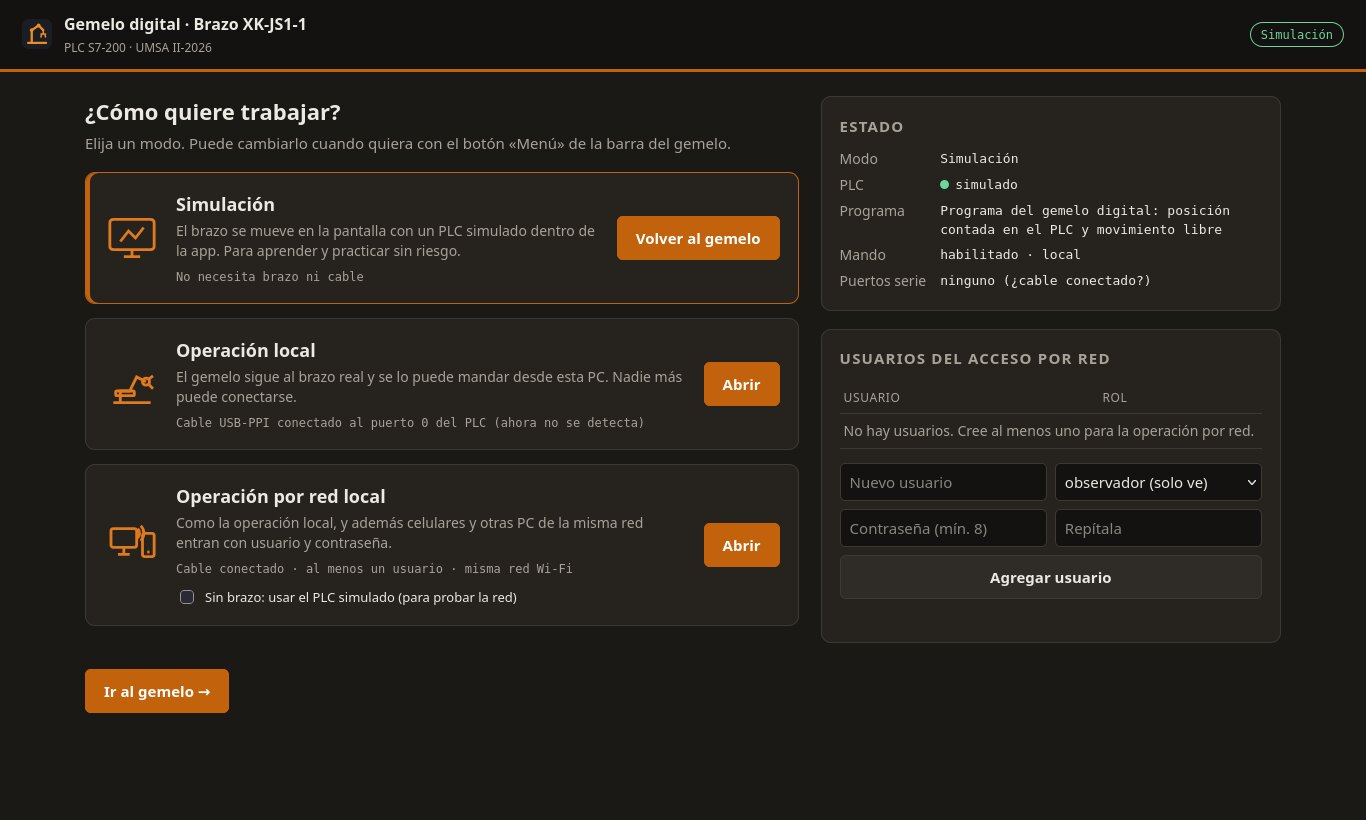
\includegraphics[width=0.85\linewidth]{menu_inicio.jpg}
\caption{Menú de la app.}
\end{figure}
\begin{lstlisting}[style=py, caption={Cambio de modo (\texttt{gemelo\_brazo.py}).}]
def aplicar_modo(modo, red_simulado=False):
    if modo == 'red' and not ACCESO.hay_usuarios():
        raise ValueError('para la operación por red cree antes al menos un usuario')
    simulado = modo == 'simulacion' or (modo == 'red' and red_simulado)
    with CAMBIO:
        if BRAZO is None or BRAZO.simulado != simulado:
            if BRAZO:
                BRAZO.cerrar()                  # detiene el brazo y suelta el puerto
            BRAZO = Brazo(Config.puerto, Config.direccion, simulado, REGISTRO)
        if modo == 'red':
            _activar_red()                      # servidor HTTPS en 0.0.0.0:8443
        else:
            _desactivar_red()
\end{lstlisting}

\subsection{API HTTP}
\begin{center}\small
\begin{longtable}{>{\ttfamily}p{4.6cm} >{\raggedright}p{2.6cm} >{\raggedright\arraybackslash}p{7.8cm}}
\toprule
\textbf{\rmfamily Ruta} & \textbf{Quién} & \textbf{Qué hace}\\
\midrule
\endhead
GET /api/estado & sesión & posición, E/S, mando, conexión (6 veces por segundo)\\
GET /api/info & sesión & programa reconocido, órdenes admitidas, transmisión\\
GET /api/sesion & sesión & usuario, rol, conectados\\
POST /api/mando & operador & tomar o soltar el mando\\
POST /api/orden/<nombre> & operador con mando & homing, mover, garra, detener, velocidad, \dots\\
POST /api/calibrar\_base & operador & calcula los pulsos por grado\\
GET /menu, GET /api/app & solo esta PC & menú y su estado\\
POST /api/app/modo & solo esta PC & cambiar de modo\\
POST /api/app/usuarios & solo esta PC & agregar, cambiar clave o rol, quitar\\
GET/POST /login, GET /salir & todos & ingreso y salida (acceso por red)\\
\bottomrule
\end{longtable}
\end{center}

\subsection{Seguridad y control de acceso por roles}\label{sec:acceso}
\begin{itemize}
\item \textbf{Dos puertas}: la local (127.0.0.1) no sale a la red y no pide contraseña; la de red (8443) exige HTTPS, usuario y rol.
\item \textbf{Roles} (RBAC): \emph{observador} solo lee; \emph{operador} puede tomar el mando. Un solo mando a la vez; cualquier operador puede dar paro.
\item \textbf{Filtros de cada orden}: sesión válida, origen de la propia página (contra sitios ajenos), rol, mando, selector en automático, homing previo; y luego los límites del PLC.
\item \textbf{Contraseñas}: PBKDF2-SHA256, 200\,000 iteraciones, sal aleatoria por usuario; \codigo{usuarios.json} no se sube al repositorio.
\item \textbf{Registro}: cada ingreso, orden aceptada u orden rechazada queda en \codigo{registro\_gemelo.log}.
\end{itemize}

\section{La página publicada}
\begin{figure}[H]
\centering
\begin{tikzpicture}[node distance=5mm and 9mm]
\node[cajab, text width=2.6cm] (push) {\codigo{git push}\\a \codigo{main}};
\node[caja, text width=3.2cm, right=of push, yshift=8mm] (gha) {GitHub Actions\\\codigo{pages.yml}:\\\codigo{build-catalog.js}};
\node[caja, text width=3.2cm, right=of push, yshift=-8mm] (cf) {Cloudflare Pages:\\\codigo{build-catalog.js}};
\node[cajan, text width=3.6cm, right=of gha] (ghp) {GitHub Pages};
\node[cajan, text width=3.6cm, right=of cf] (cfp) {\codigo{brazo-4gdl-gemelo-}\\\codigo{digital.pages.dev}};
\draw[flecha] (push) -- (gha); \draw[flecha] (push) -- (cf); \draw[flecha] (gha) -- (ghp); \draw[flecha] (cf) -- (cfp);
\end{tikzpicture}
\caption{Publicación automática de la página en cada \texttt{push} a \texttt{main}.}
\end{figure}
\codigo{scripts/build-catalog.js} recorre \codigo{global/} y \codigo{semestres/} y genera \codigo{web/data/catalogo.js}, el índice de documentos, programas y fotos que muestra la página. Los títulos y descripciones se corrigen en \codigo{config/archivos.json}. La sección \emph{Modelo 3D} de la página es la misma que usa la app (\codigo{web/js/modelo3d.js}, \codigo{cinematica.js}, \codigo{conexion-plc.js} y three.js 0.160).

\begin{figure}[H]
\centering
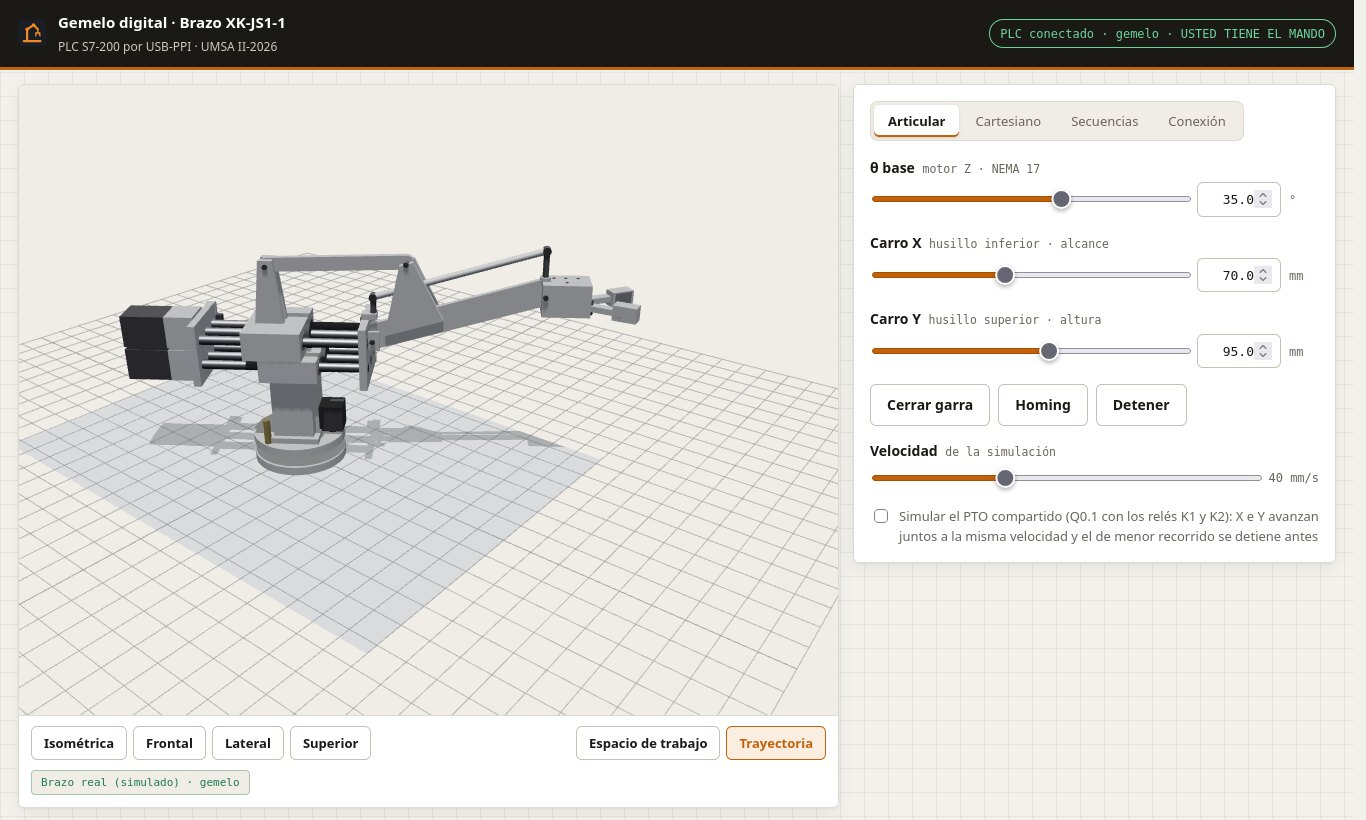
\includegraphics[width=0.85\linewidth]{local_articular.jpg}
\caption{Página del gemelo dentro de la app (modo simulación).}
\end{figure}

% =====================================================================
\chapter{Base de datos}\label{cap:datos}

\section{Requerimientos}
Del levantamiento del informe 1 (ETN-1000) y de lo que la app ya produce, la base debe guardar:
\begin{itemize}
\item la \textbf{telemetría} de las variables (PV, MV) con marca de tiempo: posiciones de los ejes, frecuencias;
\item los \textbf{cambios de estado} de las señales digitales (finales de carrera, relés, garra);
\item los \textbf{ciclos de operación}: cuándo y en qué modo se usó la planta y con qué programa;
\item las \textbf{órdenes} (acciones de control): quién, cuándo, qué, con qué destinos, aceptada o rechazada y por qué;
\item las \textbf{alarmas}: watchdog, paro, falla de homing, fuera de rango\dots;
\item los \textbf{usuarios, roles e ingresos} (registro de sesiones).
\end{itemize}

\section{Del modelo preliminar al modelo normalizado}
\begin{figure}[H]
\centering
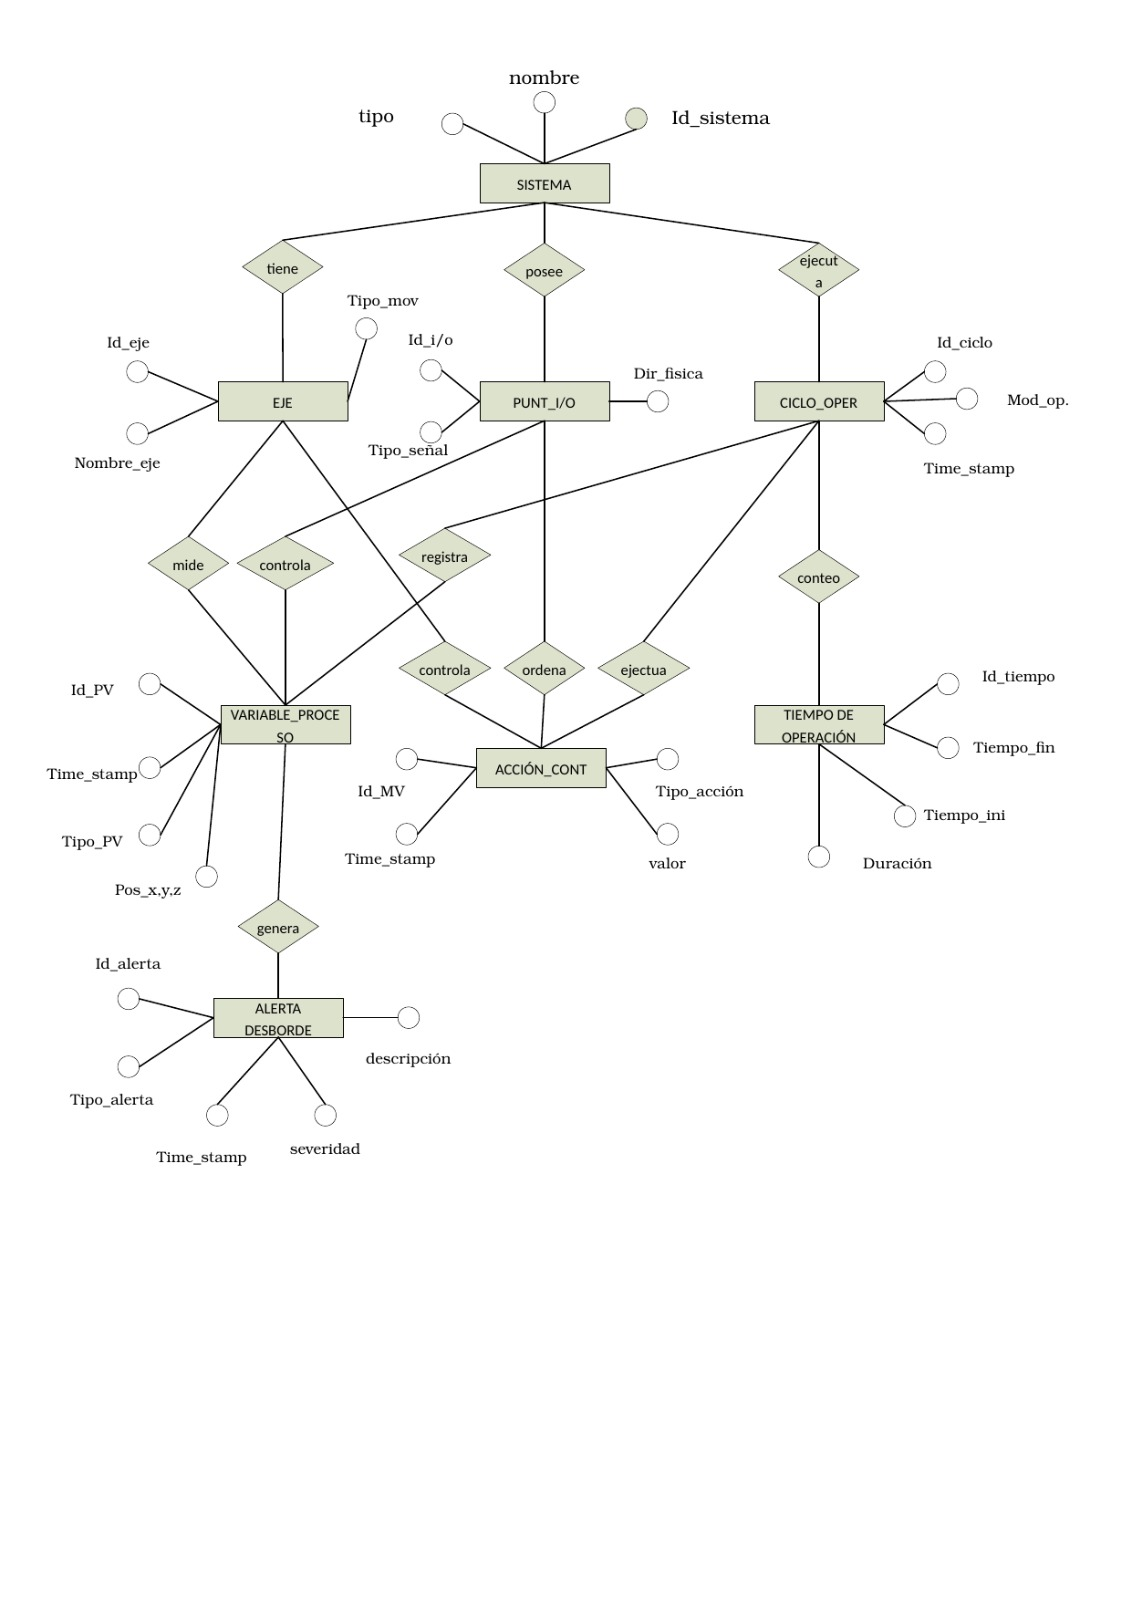
\includegraphics[width=0.62\linewidth, trim=0 360 0 0, clip]{modelo_er_preliminar.png}
\caption{Modelo E-R preliminar del equipo (\texttt{base-de-datos/modelo/}).}
\end{figure}

Cambios para llevarlo a 3FN y a la planta real:
\begin{center}\small
\begin{tabularx}{\linewidth}{>{\raggedright}p{4.4cm} >{\raggedright\arraybackslash}X}
\toprule
\textbf{Preliminar} & \textbf{Normalizado}\\
\midrule
VARIABLE\_PROCESO con \emph{Pos\_x.y.z} & 1FN: un valor por fila; la variable (tag, unidad, rango) está en \codigo{variable} y cada medición en \codigo{muestra}\\
ACCION\_CONT con \emph{valor} & la orden en \codigo{orden}; sus destinos, uno por eje, en \codigo{orden\_parametro} (1FN)\\
TIEMPO DE OPERACIÓN con \emph{Duración} & 3FN: la duración depende de inicio y fin; no se guarda, se calcula en la vista \codigo{v\_ciclo}\\
ALERTA DESBORDE & catálogo \codigo{alarma} (código, severidad) + \codigo{evento\_alarma} (cuándo se activó)\\
PUNT\_I/O & \codigo{punto\_io} con dirección del PLC, tag ISA y eje\\
(no existía) & \codigo{usuario}, \codigo{rol}, \codigo{sesion}: control de acceso y registro de ingresos (guías 3 y Fase 3)\\
(no existía) & \codigo{programa\_plc}: qué programa estaba cargado en cada ciclo\\
\bottomrule
\end{tabularx}
\end{center}

\section{Modelo lógico}\label{sec:tablas}
\begin{figure}[H]
\centering
\begin{tikzpicture}[x=1cm,y=1cm, rel/.style={thick, black!60}, card/.style={font=\tiny\bfseries, fill=white, inner sep=1pt}]
\node[tabla] (sis) at (0,0) {\textbf{sistema}\nodepart{two}PK id\\nombre, tipo, plc};
\node[tabla] (eje) at (4.2,0) {\textbf{eje}\nodepart{two}PK id\\FK sistema\_id\\codigo, nombre, tipo\_mov\\unidad, pulsos\_unidad, lazo\_isa};
\node[tabla] (pio) at (8.4,0) {\textbf{punto\_io}\nodepart{two}PK id\\FK sistema\_id, FK eje\_id\\direccion, tag\_isa (UQ)\\tipo\_senal, descripcion};
\node[tabla] (var) at (4.2,-3.1) {\textbf{variable}\nodepart{two}PK id\\FK eje\_id\\tag\_isa (UQ), clase PV/MV/DV\\nombre, unidad, rango};
\node[tabla] (prog) at (0,-3.1) {\textbf{programa\_plc}\nodepart{two}PK id\\nombre, perfil\_app\\firma, descripcion};
\node[tabla] (ciclo) at (0,-6.2) {\textbf{ciclo\_operacion}\nodepart{two}PK id\\FK sistema\_id\\FK programa\_id\\modo, inicio, fin};
\node[tabla] (mue) at (4.2,-6.2) {\textbf{muestra}\nodepart{two}PK id\\FK ciclo\_id, FK variable\_id\\instante, valor};
\node[tabla] (est) at (8.4,-3.1) {\textbf{estado\_io}\nodepart{two}PK id\\FK ciclo\_id, FK punto\_id\\instante, valor};
\node[tabla] (ord) at (0,-9.3) {\textbf{orden}\nodepart{two}PK id\\FK ciclo\_id, FK usuario\_id\\instante, tipo\\aceptada, motivo};
\node[tabla] (op) at (4.2,-9.3) {\textbf{orden\_parametro}\nodepart{two}PK (orden\_id, eje\_id)\\valor};
\node[tabla] (ala) at (8.4,-9.3) {\textbf{alarma}\nodepart{two}PK id\\codigo (UQ), severidad\\descripcion};
\node[tabla] (eva) at (8.4,-6.2) {\textbf{evento\_alarma}\nodepart{two}PK id\\FK alarma\_id, FK ciclo\_id\\instante, activa, detalle};
\node[tabla] (rol) at (0,-12.2) {\textbf{rol}\nodepart{two}PK id\\nombre (UQ)};
\node[tabla] (usu) at (4.2,-12.2) {\textbf{usuario}\nodepart{two}PK id\\FK rol\_id\\nombre (UQ), clave\_hash};
\node[tabla] (ses) at (8.4,-12.2) {\textbf{sesion}\nodepart{two}PK id\\FK usuario\_id\\ip, instante, exito, fin};
\draw[rel] (sis) -- node[card, pos=0.2]{1} node[card, pos=0.8]{N} (eje);
\draw[rel] (eje) -- node[card, pos=0.2]{1} node[card, pos=0.8]{N} (pio);
\draw[rel] (eje) -- node[card, pos=0.2]{1} node[card, pos=0.8]{N} (var);
\draw[rel] (sis.south west) ++(0.2,0) |- ([yshift=4mm]ciclo.west) ;
\draw[rel] (prog) -- node[card, pos=0.2]{1} node[card, pos=0.8]{N} (ciclo);
\draw[rel] (ciclo) -- node[card, pos=0.2]{1} node[card, pos=0.8]{N} (mue);
\draw[rel] (var) -- node[card, pos=0.2]{1} node[card, pos=0.8]{N} (mue);
\draw[rel] (pio) -- node[card, pos=0.2]{1} node[card, pos=0.8]{N} (est);
\draw[rel] (ciclo.east) ++(0,0.3) -- node[card, pos=0.1]{1} node[card, pos=0.9]{N} (est.west);
\draw[rel] (ciclo) -- node[card, pos=0.2]{1} node[card, pos=0.8]{N} (ord);
\draw[rel] (ord) -- node[card, pos=0.2]{1} node[card, pos=0.8]{N} (op);
\draw[rel] (eje.south east) ++(-0.3,0) -- ++(0,-0.2) -- ([xshift=12mm]op.north);
\draw[rel] (ala) -- node[card, pos=0.2]{1} node[card, pos=0.8]{N} (eva);
\draw[rel] (ciclo.east) ++(0,-0.3) -- (eva.west);
\draw[rel] (rol) -- node[card, pos=0.2]{1} node[card, pos=0.8]{N} (usu);
\draw[rel] (usu) -- node[card, pos=0.2]{1} node[card, pos=0.8]{N} (ses);
\draw[rel] (usu.north west) ++(0.3,0) -- ([xshift=-10mm]ord.south east);
\end{tikzpicture}
\caption{Modelo lógico normalizado (PostgreSQL). PK: clave primaria; FK: clave foránea; UQ: único; 1--N: cardinalidad.}
\end{figure}

\section{Por qué está en tercera forma normal}
\begin{itemize}
\item \textbf{1FN} (valores atómicos, sin grupos repetidos): la posición $(X, Y, Z)$ no va en una celda; cada variable es una fila de \codigo{variable} y cada medición una fila de \codigo{muestra}. Los destinos de una orden van en \codigo{orden\_parametro}, una fila por eje.
\item \textbf{2FN} (sin dependencias parciales): todas las tablas tienen clave simple salvo \codigo{orden\_parametro}, cuyo único atributo \codigo{valor} depende de la clave completa (orden y eje).
\item \textbf{3FN} (sin dependencias transitivas): la unidad y el rango dependen de la variable, no de la muestra; el rol depende del usuario, no de la sesión; la duración de un ciclo depende de inicio y fin y por eso se calcula.
\end{itemize}

\section{El script SQL}
El script \codigo{base-de-datos/scripts/brazo\_4gdl.sql} crea las 15 tablas con sus restricciones, un trigger, dos vistas y carga los datos fijos de la planta: sistema, 4 ejes, 22 señales del PLC con sus tags ISA, 5 variables, 3 programas, 8 alarmas y 2 roles. El listado completo está en el apéndice \ref{ap:sql}.

\begin{lstlisting}[style=sql, caption={Trigger que rechaza muestras fuera de rango (lo pide la guía 1 para la Fase 2).}]
CREATE FUNCTION validar_muestra() RETURNS trigger AS $$
DECLARE
    r variable%ROWTYPE;
BEGIN
    SELECT * INTO r FROM variable WHERE id = NEW.variable_id;
    IF NEW.valor < r.rango_min OR NEW.valor > r.rango_max THEN
        RAISE EXCEPTION 'muestra fuera de rango para % (%): % no está en [%, %]',
            r.tag_isa, r.unidad, NEW.valor, r.rango_min, r.rango_max;
    END IF;
    RETURN NEW;
END;
$$ LANGUAGE plpgsql;
CREATE TRIGGER muestra_en_rango BEFORE INSERT OR UPDATE ON muestra
    FOR EACH ROW EXECUTE FUNCTION validar_muestra();
\end{lstlisting}

\section{De la app a las tablas}
\begin{center}\small
\begin{tabularx}{\linewidth}{>{\raggedright}p{5.4cm} >{\raggedright\arraybackslash}X}
\toprule
\textbf{Dato que ya produce la app} & \textbf{Tabla}\\
\midrule
cambio de modo en el menú & \codigo{ciclo\_operacion} (inicio/fin, modo, programa reconocido)\\
\codigo{/api/estado}: \codigo{theta\_deg}, \codigo{sX\_mm}, \codigo{sY\_mm} & \codigo{muestra} con las variables ZI-101, ZI-102, ZI-103\\
\codigo{/api/estado}: entradas y salidas & \codigo{estado\_io} (solo los cambios)\\
línea \codigo{orden mover \{...\} (usuario)} del registro & \codigo{orden} + \codigo{orden\_parametro}\\
línea \codigo{RECHAZADO ...} & \codigo{orden} con \codigo{aceptada = false} y su motivo\\
error del PLC (VB1123), pérdida de comunicación & \codigo{evento\_alarma}\\
\codigo{usuarios.json} & \codigo{usuario} y \codigo{rol} (mismo hash PBKDF2)\\
líneas \codigo{ingreso de ...} / \codigo{ingreso fallido} & \codigo{sesion}\\
\bottomrule
\end{tabularx}
\end{center}

\begin{lstlisting}[style=sql, caption={Consultas de ejemplo.}]
-- Posición del carro X en el último ciclo, cada segundo
SELECT date_trunc('second', m.instante) AS t, avg(m.valor) AS x_mm
FROM muestra m JOIN variable v ON v.id = m.variable_id
WHERE v.tag_isa = 'ZI-102' AND m.ciclo_id = (SELECT max(id) FROM ciclo_operacion)
GROUP BY 1 ORDER BY 1;

-- Órdenes rechazadas por usuario y motivo
SELECT u.nombre, o.motivo, count(*) FROM orden o LEFT JOIN usuario u ON u.id = o.usuario_id
WHERE NOT o.aceptada GROUP BY 1, 2 ORDER BY 3 DESC;
\end{lstlisting}

\pendiente{El script no se ejecutó todavía: la PC donde se escribió no tiene PostgreSQL. Falta: (1) crear la base y correr el script en la PC del laboratorio; (2) agregar a la app un módulo que inserte las muestras (por ejemplo, una por segundo y por eje), los cambios de E/S, las órdenes y los ingresos, con la biblioteca \codigo{psycopg}; (3) un tablero que consulte el historial.}

% =====================================================================
\chapter{Estructura del proyecto y control de versiones}\label{cap:proyecto}

\section{Repositorios}
\begin{itemize}
\item \textbf{Brazo-de-4-grados-de-libertad} (GitHub, \codigo{GabAndGom}): repositorio original del equipo, con el material de los semestres anteriores (2026\_I) y del actual.
\item \textbf{Brazo-4GDL-gemelo-digital} (GitHub, \codigo{GabAndGom}): derivado del anterior con todo su historial, agrega el gemelo digital. Publica la página en \url{https://brazo-4gdl-gemelo-digital.pages.dev}.
\end{itemize}
Regla del equipo: en el repositorio original no se modifica el material de la gestión I/2026; el trabajo nuevo va en \codigo{semestres/2026\_II/}.

\section{Árbol del repositorio}
\begin{lstlisting}
Brazo-4GDL-gemelo-digital/
|-- index.html, web/            pagina publicada: estilos, JS, imagenes
|   `-- js/  cinematica.js  modelo3d.js  conexion-plc.js  app.js
|-- scripts/build-catalog.js    genera el catalogo de archivos de la pagina
|-- config/                     titulos, semestres, videos (JSON)
|-- .github/workflows/pages.yml publicacion en GitHub Pages
|-- global/                     material que no depende del semestre
|   |-- componentes/            imagenes de cada componente
|   |-- datasheets/             PLC, drivers, sensores, reles
|   |-- fotos-planta/           fotos del brazo y del tablero
|   |-- manuales/               manual del fabricante, referencia ladder, MAP_SERV
|   |-- modelo-3d/              brazo_xk-js1-1.glb y su generador
|   |-- normativas/             ISA-5.1, IEC 60617
|   |-- plantillas/             plantilla LaTeX de informes
|   `-- programas-plc/          programa del fabricante, libreria MAP_SERV
`-- semestres/
    |-- 2026_I/                 gestion anterior (no se modifica)
    `-- 2026_II/
        |-- guias/              guias de laboratorio 1, 2 y 3
        |-- informes/           informe 1 (auditoria y requerimientos)
        |-- diagramas/          diagrama de bloques fenomenologico
        |-- planos/electrico/, planos/pid/   planos .dwg (historico)
        |-- base-de-datos/      mockups, modelo E-R, scripts SQL, interfaz
        |-- modelo-3d/          levantamiento, cinematica, informe y figuras
        |-- programas-plc/      programa original de secuencias (.awl, .mwp)
        |-- gemelo-digital/
        |   |-- app/            app unificada (Linux y Windows)
        |   |-- plc/            brazo_gemelo.awl y .mwp
        |   `-- manual/         manuales, arquitectura, guia y este manual
        |-- hmi/, pruebas/, evidencias/   (README con lo que va en cada una)
\end{lstlisting}

\begin{center}\small
\begin{tabularx}{\linewidth}{>{\raggedright}p{6.4cm} >{\raggedright\arraybackslash}X}
\toprule
\textbf{Carpeta pedida en la guía 3} & \textbf{Equivalente en el repositorio}\\
\midrule
\codigo{/documentacion/planos\_isa/} & \codigo{semestres/2026\_II/planos/} (eléctrico y P\&ID)\\
\codigo{/documentacion/manuales\_inversa/} & \codigo{semestres/2026\_II/informes/}, \codigo{modelo-3d/levantamiento/}, \codigo{global/datasheets/}\\
\codigo{/database/scripts/} & \codigo{semestres/2026\_II/base-de-datos/scripts/}\\
\bottomrule
\end{tabularx}
\end{center}

\section{Archivos fuera del repositorio}
\begin{center}\small
\begin{tabularx}{\linewidth}{>{\raggedright}p{5cm} >{\raggedright\arraybackslash}X}
\toprule
\textbf{Carpeta (en \codigo{ETN 1034/})} & \textbf{Contenido}\\
\midrule
\codigo{gemelo\_brazo\_app/} y \codigo{.zip} & app exportada lista para usar, con los datos propios de la PC: usuarios, certificado, calibración, registro\\
\codigo{respaldo\_vm/} & copias de los programas encontrados en la máquina virtual (programa cargado, «BRAZO MIGUEL ROBADO», programas de semestres anteriores)\\
máquina virtual «WINDOWS XP» & STEP 7-Micro/WIN; carpeta compartida \codigo{\textbackslash\textbackslash vboxsvr\textbackslash MIS\_COSAS}\\
\bottomrule
\end{tabularx}
\end{center}
Los datos propios de cada PC (\codigo{usuarios.json}, \codigo{tls\_*.pem}, \codigo{registro\_gemelo.log}) están en \codigo{.gitignore}: nunca se suben.

\section{Flujo de trabajo con Git}
\begin{figure}[H]
\centering
\begin{tikzpicture}[x=1cm,y=1cm]
\draw[very thick, naranja] (0,0) -- (13,0) node[right, font=\scriptsize\ttfamily]{main};
\foreach \x in {0.5,2,6.5,8,11.5} \fill[naranja] (\x,0) circle (0.12);
\draw[thick, azulg] (2,0) .. controls (2.5,1) .. (3.2,1) -- (5.6,1) .. controls (6.2,1) .. (6.5,0);
\foreach \x in {3.2,4.4,5.6} \fill[azulg] (\x,1) circle (0.1);
\node[font=\scriptsize\ttfamily, above] at (4.4,1.1) {feature/ladder-s7200-homing};
\draw[thick, verde] (8,0) .. controls (8.5,-1) .. (9.2,-1) -- (10.6,-1) .. controls (11.2,-1) .. (11.5,0);
\foreach \x in {9.2,10.6} \fill[verde] (\x,-1) circle (0.1);
\node[font=\scriptsize\ttfamily, below] at (9.9,-1.1) {feature/db-y-supervision};
\node[etiq] at (6.5,0.45) {pull request\\revisado};
\node[etiq] at (13,-0.6) {push $\Rightarrow$ página publicada};
\end{tikzpicture}
\caption{Ramas de trabajo que se integran a \texttt{main} con revisión.}
\end{figure}

\begin{lstlisting}
git checkout -b feature/planos-v2-kaizen         # rama aislada para un componente
git add semestres/2026_II/planos/electrico/brazo_electrico_v2.dwg
git commit -m "Plano electrico v2.0: DIR+ de X e Y y garra corregidos"
git push origin feature/planos-v2-kaizen           # luego: Pull Request en GitHub
git log --oneline --graph                          # historial para el informe
\end{lstlisting}

\begin{center}\small
\begin{tabular}{@{}ll@{}}
\toprule
\textbf{Dato del historial} & \textbf{Valor (10/11/2026)}\\
\midrule
commits en \codigo{main} & 49 y los de este manual\\
integrantes con commits & 5 (Gabriel Gómez, José Lenin Mamani, Román Machicado, Eduardo Chura, \dots)\\
ramas de trabajo & \codigo{feature/ladder-s7200-homing}, \codigo{feature/db-y-supervision}, \codigo{feature/planos-v2-kaizen}, \codigo{feat/cinematica-modelo-3d}\\
primer commit & 28/09/2026\\
\bottomrule
\end{tabular}
\end{center}

\section{Convenciones}
\begin{itemize}
\item \textbf{Programas del PLC}: un archivo por versión con el número en el nombre (\codigo{brazo\_secuencias\_original\_v1.awl}); exportar siempre también el AWL para que el código se pueda leer y comparar.
\item \textbf{Mensajes de commit}: en castellano, en presente, diciendo qué cambia y por qué.
\item \textbf{Fuentes y compilados}: los documentos se guardan en LaTeX con su PDF; los archivos auxiliares de compilación están en \codigo{.gitignore}.
\item \textbf{Medidas}: cada dato lleva su origen (leída, estimada, SUPUESTO).
\end{itemize}

% =====================================================================
\chapter{Variables medidas y resultados}\label{cap:mediciones}

\section{Datos medidos o verificados en la planta}
\begin{center}\small
\begin{longtable}{>{\raggedright}p{5.2cm} >{\raggedright}p{3.6cm} >{\raggedright\arraybackslash}p{6cm}}
\toprule
\textbf{Magnitud} & \textbf{Valor} & \textbf{Cómo y cuándo}\\
\midrule
\endhead
\multicolumn{3}{@{}l}{\textbf{Eléctricas} (informe 1, agosto de 2026, multímetro)}\\
entradas de la botonera & 21,6~V accionado / 23,1~V reposo & medición pasiva en bornes\\
salida de la garra Q0.7 & 23,2~V / 0,2~V & ídem\\
rieles del PLC & 5,1--23,7~V & ídem\\
\multicolumn{3}{@{}l}{\textbf{Configuración} (26/10/2026)}\\
DIP de los tres drivers & OFF OFF ON OFF ON ON ON OFF & foto del tablero\\
corriente de X e Y & 2,37~A pico / 1,69~A RMS & tabla DM542\\
resolución & 1000 pulsos/vuelta & tabla DM542/JMC\\
recorrido de los carros & 170~mm (34\,000 pulsos) & dato del equipo, coincide con la geometría\\
\multicolumn{3}{@{}l}{\textbf{Mapeo de señales} (26/10/2026, monitor PPI y accionamiento manual)}\\
finales de carrera & I0.1--I0.4 & cada sensor accionado a mano\\
inductivo de la base & I0.0 & ídem\\
sentido de X & Q0.3 = 0 adelante & jog con I1.2\\
\multicolumn{3}{@{}l}{\textbf{Comunicación}}\\
programa original & PPI dirección 6, 19,2~kbit/s & búsqueda automática, 26/10/2026\\
con \codigo{brazo\_gemelo} & PPI dirección 2, 9,6~kbit/s & 27/10/2026\\
lectura E/S + VB1000--1011 a 19,2~kbit/s & 145~ms & cliente PPI, solo lectura\\
lectura de 40 bytes a 9,6~kbit/s & 568~ms $\rightarrow$ 155~ms & antes y después del silencio entre tramas\\
\multicolumn{3}{@{}l}{\textbf{Calibración}}\\
base & 190,3 pulsos/grado & giro medido con transportador, 26/10/2026 (\codigo{calibracion.json})\\
\bottomrule
\end{longtable}
\end{center}

\section{Pruebas realizadas}
\begin{center}\small
\begin{longtable}{>{\raggedright}p{5.6cm} >{\raggedright\arraybackslash}p{9.4cm}}
\toprule
\textbf{Prueba} & \textbf{Resultado}\\
\midrule
\endhead
Cinemática: directa seguida de inversa en toda la grilla de carreras (\codigo{pruebas\_cinematica.js}) & devuelve el mismo $q$\\
Modelo frente a fotos del manual y de la planta & diferencia menor a 5~mm en los pivotes B y C\\
Estimador con el programa original (\codigo{pruebas\_estimador.py}) & error máximo 1,35~mm en X/Y; autocalibración del jog\\
Compilación de \codigo{brazo\_gemelo} en Micro/WIN & 0 errores; cargado en el PLC\\
App con el brazo real (programa del gemelo) & conexión estable a 9,6~kbit/s, sin cortes\\
Cliente PPI contra un PLC falso (pseudoterminal) & lecturas, escrituras y protección de zonas correctas\\
Acceso por red: roles y filtros & observador rechazado al mover y al tomar el mando; operador sin mando rechazado; mover sin homing rechazado\\
App unificada en modo simulado & menú, alta de usuarios, cambio entre los tres modos, acceso remoto; el menú no es accesible desde la red\\
Certificado HTTPS generado en Python & validado con OpenSSL; conexión TLS correcta\\
\bottomrule
\end{longtable}
\end{center}

\section{Validación del gemelo}
El hito de la Fase 2 pide gemelos validados en simulación. En el brazo:
\begin{itemize}
\item la geometría del modelo reproduce las fotos con menos de 5~mm de diferencia;
\item el PLC simulado reproduce el comportamiento de \codigo{brazo\_gemelo} (mismos pasos, errores y tiempos) y permite probar toda la app sin hardware;
\item con el programa del gemelo cargado, la posición del modelo es la contada por el PLC (exacta al pulso mientras no se pierdan pasos).
\end{itemize}
\pendiente{Medir con regla o calibre el error de posición de la garra en varios puntos del espacio de trabajo y verificar el paso del husillo (SUPUESTO de 5~mm), las cotas estimadas del mecanismo y el sentido de la base.}

% =====================================================================
\chapter{Cumplimiento de los objetivos de las guías}\label{cap:cumplimiento}

\begin{center}\small
\begin{longtable}{>{\raggedright}p{6.4cm} >{\raggedright}p{1.8cm} >{\raggedright\arraybackslash}p{6.8cm}}
\toprule
\textbf{Objetivo} & \textbf{Estado} & \textbf{Evidencia o lo que falta}\\
\midrule
\endhead
\multicolumn{3}{@{}l}{\textbf{Laboratorio 1: auditoría}}\\
Clasificar variables PV, MV, DV & \cumple & capítulo \ref{cap:planta}, corregido con la planta en marcha\\
Ficha técnica del hardware & \cumple & capítulos \ref{cap:planta} y \ref{cap:drivers}\\
Ruptura de causalidad, lazo abierto & \cumple & sección del capítulo \ref{cap:planta}\\
Arquitectura de 3 capas & \cumple & capítulo \ref{cap:aplicaciones}\\
\multicolumn{3}{@{}l}{\textbf{Laboratorio 2: planos e interfaces}}\\
Plano eléctrico versión 2.0 en AutoCAD Electrical & \falta & discrepancias documentadas (sección \ref{sec:kaizen}) y esquema funcional (capítulo \ref{cap:electrico}); falta dibujar el \codigo{.dwg} v2.0\\
P\&ID con tags ISA-5.1 & \parcial & tags propuestos (capítulo \ref{cap:planta}); falta el plano\\
Mockups HMI y dashboard & \parcial & mockups del equipo en \codigo{base-de-datos/mockups/}; la app y la página son la interfaz real\\
\multicolumn{3}{@{}l}{\textbf{Laboratorio 3: Git y modelo de datos}}\\
Repositorio estructurado, ramas y pull requests & \cumple & capítulo \ref{cap:proyecto}\\
Modelo E-R normalizado en 3FN & \cumple & capítulo \ref{cap:datos}\\
Scripts en \codigo{/database/scripts/} & \parcial & \codigo{brazo\_4gdl.sql} escrito; falta ejecutarlo en PostgreSQL\\
\multicolumn{3}{@{}l}{\textbf{Fase 2: modelado y backend}}\\
Modelado y linealización del brazo & \cumple & capítulo \ref{cap:cinematica}: jacobiano y linealización con errores medidos\\
Redes de Petri & \cumple & sección \ref{sec:petri}\\
Triggers contra datos fuera de rango & \parcial & trigger escrito; falta probarlo\\
Gemelo validado en simulación & \cumple & capítulo \ref{cap:mediciones}\\
\multicolumn{3}{@{}l}{\textbf{Fase 3: implementación}}\\
Programa del PLC con PTO y comunicación & \cumple & capítulo \ref{cap:gemeloplc}\\
Comunicación PLC--PC por tramas binarias & \cumple & capítulo \ref{cap:ppi} (PPI en lugar de Modbus, justificado)\\
Middleware en Python & \cumple & capítulo \ref{cap:aplicaciones}\\
Control de acceso por roles & \cumple & sección \ref{sec:acceso}\\
Lazo cerrado en el hardware & \falta & sin encoders: el brazo sigue en lazo abierto con supervisión discreta\\
Telemetría en PostgreSQL y dashboard & \falta & diseño listo; falta conectar la app a la base\\
\bottomrule
\end{longtable}
\end{center}

\section{Siguientes pasos}
\begin{enumerate}
\item Dibujar los planos versión 2.0 con las discrepancias corregidas.
\item Instalar PostgreSQL, ejecutar el script y agregar a la app el registro de telemetría.
\item Implementar rampas en el PTO y subir la corriente de X e Y.
\item Medir el error de posición de la garra y verificar los SUPUESTOS.
\item Agregar encoders (o el contador rápido HSC del PLC) para cerrar el lazo de posición.
\end{enumerate}


\appendix
% =====================================================================
\chapter{Programa original de secuencias (AWL completo)}\label{ap:original}
Archivo \codigo{semestres/2026\_II/programas-plc/brazo\_secuencias\_original\_v1.awl}.
\lstinputlisting[style=awl]{../../../programas-plc/brazo_secuencias_original_v1.awl}

\chapter{Programa \texttt{brazo\_gemelo} (AWL completo)}\label{ap:gemelo}
Archivo \codigo{semestres/2026\_II/gemelo-digital/plc/brazo\_gemelo.awl}.
\lstinputlisting[style=awl]{../../plc/brazo_gemelo.awl}

\chapter{Script de la base de datos}\label{ap:sql}
Archivo \codigo{semestres/2026\_II/base-de-datos/scripts/brazo\_4gdl.sql}.
\lstinputlisting[style=sql]{../../../base-de-datos/scripts/brazo_4gdl.sql}


\end{document}
